%2multibyte Version: 5.50.0.2960 CodePage: 932
% \graphicspath{ {/Users/bb779/Dropbox/Research/wisconsin_competition/out/} }
%reference relative to PaperDraft folder so all computers work

\documentclass[notitlepage,12pt]{article}%
\usepackage{amssymb}
\usepackage{geometry}
\usepackage[onehalfspacing]{setspace}
\usepackage{amsmath}
\usepackage{amsfonts}
\usepackage{natbib}
\usepackage{graphicx}
\usepackage{caption}
\usepackage{subcaption}%
\setcounter{MaxMatrixCols}{30}
%TCIDATA{OutputFilter=latex2.dll}
%TCIDATA{Version=5.50.0.2960}
%TCIDATA{Codepage=932}
%TCIDATA{CSTFile=40 LaTeX article.cst}
%TCIDATA{Created=Monday, February 16, 2009 12:45:38}
%TCIDATA{LastRevised=Monday, February 24, 2025 16:01:07}
%TCIDATA{<META NAME="GraphicsSave" CONTENT="32">}
%TCIDATA{<META NAME="SaveForMode" CONTENT="3">}
%TCIDATA{BibliographyScheme=Manual}
%TCIDATA{<META NAME="DocumentShell" CONTENT="Standard LaTeX\Blank - Standard LaTeX Article">}
%TCIDATA{Language=American English}
%TCIDATA{ComputeDefs=
%1$b_{m}=E\left(  e^{\zeta}\right)  \sum_{\tau^{\prime}=\omega}^{T}\delta
%^{\tau^{\prime}-1}e^{\left(  \alpha_{0m}+\alpha_{1m}(\tau^{\prime}%
%-3)-\alpha_{2m}(\tau^{\prime}-3)^{2}\right)  }$
%}
%BeginMSIPreambleData
\providecommand{\U}[1]{\protect\rule{.1in}{.1in}}
%EndMSIPreambleData
\newtheorem{theorem}{Theorem}
\newtheorem{acknowledgement}{Acknowledgement}
\newtheorem{algorithm}{Algorithm}
\newtheorem{axiom}{Axiom}
\newtheorem{case}{Case}
\newtheorem{claim}{Claim}
\newtheorem{conclusion}{Conclusion}
\newtheorem{condition}{Condition}
\newtheorem{conjecture}{Conjecture}
\newtheorem{corollary}{Corollary}
\newtheorem{criterion}{Criterion}
\newtheorem{definition}{Definition}
\newtheorem{example}{Example}
\newtheorem{exercise}{Exercise}
\newtheorem{lemma}{Lemma}
\newtheorem{notation}{Notation}
\newtheorem{problem}{Problem}
\newtheorem{proposition}{Proposition}
\newtheorem{remark}{Remark}
\newtheorem{solution}{Solution}
\newtheorem{summary}{Summary}
\newenvironment{proof}[1][Proof]{\noindent\textbf{#1.} }{\ \rule{0.5em}{0.5em}}
\geometry{left=1.in,right=1.in,top=1.in,bottom=1in}
\makeatletter
\def\@biblabel#1{\hspace*{-\labelsep}}
\makeatother
\graphicspath{ {../out/} }
%BeginMSIPreambleData
\ifx\pdfoutput\relax\let\pdfoutput=\undefined\fi
\newcount\msipdfoutput
\ifx\pdfoutput\undefined\else
\ifcase\pdfoutput\else
\msipdfoutput=1
\ifx\paperwidth\undefined\else
\ifdim\paperheight=0pt\relax\else\pdfpageheight\paperheight\fi
\ifdim\paperwidth=0pt\relax\else\pdfpagewidth\paperwidth\fi
\fi\fi\fi
%EndMSIPreambleData
\begin{document}

\title{Equilibrium in the Market for Public School Teachers: District Wage Strategies
and Teacher Comparative Advantage\\(Online Appendix)}
\author{Barbara Biasi, Chao Fu and John Stromme\thanks{Biasi: Yale School of
Management and NBER, barbara.biasi@yale.edu; Fu: University of Wisconsin and NBER, cfu@ssc.wisc.edu;
Stromme: Vanderbilt University, john.stromme@vanderbilt.edu. } }
%\date{March 2025}
\maketitle

\setcounter{table}{0} \setcounter{figure}{0}
\renewcommand{\thesection}{B\arabic{section}}
\renewcommand{\thetable}{B\MakeUppercase{\arabic{table}}} \renewcommand{\thefigure}{B\MakeUppercase{\arabic{figure}}}

%%% DATA


\section{Data Details}

\subsection{Sample Construction}

We construct our samples as follows. For estimation and empirical analysis, we
focus on full-time Grades 4-6 math teachers employed in Wisconsin school
districts in 2014 (411 districts and 6,625 individuals).\footnote{Wisconsin
had 424 school districts in 2014, 11 of which did not have any elementary
school, and 2 of which did not have any full-time Grades 4-6 math teachers.}
We exclude 3 teachers from the sample, whose schools did not report test
scores. We also exclude 22 teachers with missing information on years of
experience. This leaves us with 6,600 teachers and 411 districts in the final
estimation sample. \newline For the validation sample, we focus on 6,751
full-time Grades 4-6 math teachers employed in 411 districts in 2010. We
exclude 10 teachers with missing information on years of experience. This
leaves us with 6,741 teachers and 411 districts in the final validation sample.

\subsection{Teacher's Previous District}

Our model requires identifying the district where each teacher was working at
the beginning of the model period ($d_{i0}$). For the estimation sample, which
is based on 2014 data, we define $d_{i0}$ as follows. If the teacher never
moved or moved only once between 2011 and 2014, $d_{i0}$ is the district where
she was employed in 2011. If a teacher moved more than once between 2011 and
2014, we set $d_{i0}$ to be the last employer she worked for before 2014. For
example, if teacher $i$ worked in District A in 2011 and 2012, and District C
in 2013 and 2014, then $d_{i0}=C$. If teacher $i$ worked in District A in 2011
and 2012, in District B in 2013, and in District C in 2014, then $d_{i0}%
=B$.\newline For the validation sample, based on data from 2010, we obtain
teachers' $d_{i0}$ following the same procedure as above, using a teacher's
employment history between 2007 and 2010.

\subsection{Teacher Effectiveness}

To construct our estimates of teacher effectiveness, we use data from 2007 until 2016. Given that we estimate our model using data from 2014, this implies that we estimate effectiveness using ``future'' test score observations. This helps us improve the precision of the effectiveness estimates, particularly for low-experience teachers, who are observed only for a few years.\footnote{Including ``future” observations can be justified on the grounds that it is correlated with other information agents may have about teachers' quality independent of actual observations on performance. We thank the editor for pointing this out.}

Students were tested on math and language in the Wisconsin Knowledge and
Concepts Examination (WKCE, 2007-2014) and Badger test (2015-2016); we focus
on their math scores. The WKCE was administered in November of each school
year, whereas the Badger test was administered in March. To account for this
change, for the years 2007--2014 we assign each student a score equal to the
average of the standardized scores for the current and the following year. The
test score data also include individual characteristics of test takers, such
as gender, race and ethnicity, socioeconomic (SES) status, migration status,
English-learner status, and disability status. 

Our data allow us to link students and teachers up to the school-grade level,
rather than the classroom level.\ To account for this data structure, we
estimate two student achievement models and derive teacher effectiveness
measures from each of them. In the following, we first describe the
achievement model used in our empirical analysis, and its estimation and
identification. The distribution of effectiveness measures estimated with this
achievement model is summarized in Tables \ref{tab:c12_exp} and
\ref{tab:contr} and Figures \ref{fig:kdens_c12} and \ref{fig:c1_c2}. Next, we
describe the alternative model, and its estimation and identification.
Finally, we show that the effectiveness measures we obtain from both models
are strongly correlated and that our auxiliary models used in our structural
estimation are robust to the choice of effectiveness measures.

\subsubsection{Achievement Model 1 (Main)}

The effectiveness measures used in our empirical analysis are estimated using
the following achievement model:%

\begin{align}
A_{kt}  &  =\gamma Z_{kt}^{s}+\sum_{i:SG_{kt}=SG_{it}^{T}}\sum_{n=1}%
^{2}I\left(  \tau_{k}=n\right)  (\rho_{n}x_{it}+v_{in})+\varepsilon
_{kt}\label{achievement_ols_A}\\
&  =\gamma Z_{kt}^{s}+\sum_{i:SG_{kt}=SG_{it}^{T}}\sum_{n=1}^{2}I\left(
\tau_{k}=n\right)  \rho_{n}x_{it}+\varphi_{kt}%
\end{align}
where $A_{kt}$ is achievement (measured as the standardized Math test score)
of student $k$ in year $t$. The vector $Z_{kt}^{s}$ contains the following:\ a
cubic polynomial of previous year's test scores, interacted with grade fixed
effects; a cubic polynomial of previous year's average test scores for $k$'s
cohort in the school, interacted with grade fixed effects; a set of student
characteristics, including gender, race and ethnicity, disability status,
English-language status, and socioeconomic status; the same average
characteristics for student $k$'s cohort; cohort size; grade-by-school fixed
effects; and year fixed effects. The variable $\varepsilon_{kt}$ is an i.i.d.
unobservable component of achievement, idiosyncratic to each student and year.
$SG_{kt}$ ($SG_{it}^{T})$ denotes the school-grade of student $k$ (teacher
$i)$ in year $t$. The variable $\tau_{k}$ equals 1 for low-achieving students
and 2 for high-achieving ones; we consider a student to be low-achieving if
their test score in the previous year was below the grade-specific median in
the state, and high-achieving otherwise. The contribution of teacher $i$ to
the achievement of a student of type $n\in\{1,2\}$ is $\rho_{n}x_{it}+v_{in}$,
where $x_{it}$ denotes $i$'s education and experience in year $t$ and $v_{in}$
is the part unexplained by $x_{it}$.

The achievement model in (\ref{achievement_ols_A}) assumes that all teachers
in a given school-grade contribute to the achievement of all students in the
same school-grade. We make this choice to be able to allow $x_{it}$ to
directly enter teacher effectiveness (since experience has been shown to
affect teacher effectiveness (Wiswall 2013), especially in the first years of
a teacher's career (Rockoff 2004)), even if we do not observe all the
teacher-student classroom links in the data. Model (\ref{achievement_ols_A})
allows us to identify the component of teacher effectiveness that depends on a
teacher's experience and education.

Constructing our measures of effectiveness $(c_{i1},c_{i2})$ requires
estimating $v_{in}$ and $\rho_{n}$ for $n\in\{1,2\}$. We make the following
two assumptions: \newline A1. $\varepsilon_{kt}$ is i.i.d. with mean 0 and
variance $\sigma_{\varepsilon}^{2}$.\newline A2. $Cov(\varepsilon_{kt}%
,v_{in})=0$ $\forall k,i,t,n:SG_{it}^{T}=SG_{kt}$. This implies that there is
no sorting on unobservables of teachers across school-grades within a
district. Although there is no direct test of this assumption, in Section
\ref{sorting} we combine the approaches of \citet{chetty2014measuring} and
\citet{rothstein2010teacher} and we do not find evidence of non-random sorting.

\paragraph{Estimation Procedure: Model 1}

\begin{enumerate}
\item Given A1 and A2, we estimate $\gamma$ and $\rho_{n}$ via OLS on equation
(\ref{achievement_ols_A}), to obtain $\hat{\gamma}$ and $\hat{\rho}_{n}.$

\item With the estimated $\hat{\gamma}$ and $\hat{\rho}_{n}$, we can then
estimate $v_{in}$ using an empirical Bayes estimator similar to the one of
\citet{kane2008estimating} which we adapt to take into account the structure
of our data.

\begin{enumerate}
\item Let
\begin{equation}
\widehat{\varphi}_{kt}=A_{kt}-\hat{\gamma}Z_{kt}^{s}-\sum_{i:SG_{kt}%
=SG_{it}^{T}}\sum_{n=1}^{2}\hat{\rho}_{n}x_{it}I(\tau_{k}=n).
\end{equation}
The quantity $\widehat{\varphi}_{kt}$ is an estimate for $\varphi_{kt},$
i.e.,
\[
\varphi_{kt}\equiv\sum_{i^{\prime}:SG_{kt}=SG_{i^{\prime}t}^{T}}\sum_{n=1}%
^{2}v_{i^{\prime}n}I(\tau_{k}=n)+\varepsilon_{kt}.
\]
Let $K_{SG_{it}^{T}n}$ be the number of achievement type-$n$ students in the
school-grade that $i$ belongs to. For each teacher $i$ we define, for
$n\in\left\{  1,2\right\}  $
\begin{equation}
\widehat{v}_{int}=\frac{1}{K_{SG_{it}^{T}n}}\sum_{k:SG_{kt}=SG_{it}^{T}%
}\widehat{\varphi}_{kt}I\left(  \tau_{k}=n\right)
\end{equation}
which is an estimate of
\[
\sum_{i^{\prime}:SG_{i^{\prime}t}^{T}=SG_{it}^{T}}v_{i^{\prime}n}+\frac
{1}{K_{SG_{it}^{T}n}}\sum_{k:SG_{kt}=SG_{it}^{T}}\varepsilon_{kt}.
\]
This quantity corresponds to the average test score residuals of type-$n$
students in teacher $i$'s school-grade in year $t$, conditional on observables
$Z_{kt}^{s}$ and the characteristics $x$ of all teachers in the same
school-grade in $t$.

\item We form a weighted average of the residuals $\left\{  \widehat{v}%
_{int}\right\}  _{t}$ by weighting each $\widehat{v}_{int}$ by $\varpi
_{int}=\frac{K_{SG_{it}^{T}n}}{\sum_{t}K_{SG_{it}^{T}n}}$, so that residuals
corresponding to more observations receive more weight:%
\begin{equation}
\bar{v}_{in}=\sum_{t}\varpi_{int}\widehat{v}_{int} \label{unshrunk}%
\end{equation}
Note that assumption A1 implies
\[
E(\bar{v}_{in})=v_{in}+\sum_{t}\varpi_{int}\sum_{i^{\prime}\neq
i:SG_{i^{\prime}t}^{T}=SG_{it}^{T}}v_{i^{\prime}n}%
\]
Taking the limit of this expectation as $t$ approaches infinity yields
\[
\lim_{t\rightarrow\infty}E(\bar{v}_{in})=v_{in}+\lim_{t\rightarrow\infty}%
\sum_{t}\varpi_{int}\sum_{i^{\prime}\neq i:SG_{i^{\prime}t}^{T}=SG_{it}^{T}%
}v_{i^{\prime}n}%
\]
It follows that a requirement for the estimator $\bar{v}_{in}^{\prime}$ to be
asymptotically unbiased is that $\lim_{t\rightarrow\infty}\sum_{t}\varpi
_{int}\sum_{i^{\prime}\neq i:SG_{i^{\prime}t}^{T}=SG_{it}^{T}}v_{i^{\prime}%
n}=0$. In words, the weighted sum of the effects of all teachers in $i$'s
school-grade over time has to approach $0$ as the number of periods grows
large. This requirement is met because 1) the teacher effect $v_{in}$ is
defined as a residual component of standardized test scores conditioning on
grade-by-school fixed effects (which implies that, across time, the mean of
$v_{in}$ is zero within each school-grade) and 2) Assumption A2 guarantees
that there is no sorting of teachers on unobservables across school-grades
over time.

\item Armed with $\bar{v}_{in}$, we can construct the empirical Bayes
estimator of $v_{in}$ by multiplying $\bar{v}_{in}$ by the shrinkage factor, a
measure of the reliability of the estimator defined as the ratio between the
estimated variance of the quantity to be estimated, $\hat{\sigma}%
_{vn}=Var(v_{in})$, and the variance of the estimator:
\[
\hat{v}_{in}=\bar{v}_{in}\left(  \frac{\widehat{\sigma}_{vn}^{2}}{Var(\bar
{v}_{in})}\right)  ,
\]
where, given assumptions A1 and A2, we can estimate $\hat{\sigma}^{2}_{vn}$
as
\[
\widehat{\sigma}_{vn}^{2}=\frac{Cov(\widehat{v}_{int},\widehat{v}_{int-1}%
)}{J_{SG_{it,t-1}^{T}}}%
\]
and $J_{SG_{it,t-1}^{T}}=\sum_{i^{\prime}}I(SG_{i^{\prime}t}^{T}=SG_{it}%
^{T})I(SG_{i^{\prime}t-1}^{T}=SG_{it-1}^{T})$ is the number of teachers who
are in the same school-grade as $i$ in both $t$ and $t-1$. The estimator $\hat{v}_{in}$ is forecast-unbiased for $v_{in}$ \citep{chetty2014measuring}.
%When classroom assignments are observable and $\hat{v}_{int}$ is defined based on classroom (rather than grade-school) residuals, $J_{SG_{it,t-1}}$ would capture the number of teachers in the same classroom as $i$ in $t$ and $t-1$, which is always 1 and we would revert back to point 3. above.

\end{enumerate}
\end{enumerate}

\paragraph{Identification: Model 1}

The identification of teacher effects $v_{in}$ leverages teacher turnover
across school-grades over time. Our identifying assumption is that turnover of
teachers across school-grades, within a district, is unrelated to $v_{in}$
(Assumption A2). Importantly, this assumption allows for the endogenous
sorting of teachers across districts based on $v_{i1}$ and $v_{i2},$ as is the
case in our model. In the estimation of $v_{in}$, this type of sorting is
accounted for by the school-grade fixed effects included in $Z_{kt}^{s}.$

Teacher turnover across school-grades allows us to identify $v_{in}$ from
$\bar{v}_{in}$ for all $i$ and $n$. In particular, we can stack all the
equations (\ref{unshrunk}) for all $I$ teachers and $n=1,2,$ forming a system
of $2I$ equations (where $I$ is the total number of teachers) in $2I$ unknowns
($\{v_{in}\}_{i,n\in\{1,2\}}$). Identification is achieved if the rank
condition of the system is satisfied, i.e., if the coefficient matrix of the
system is full-rank.

In practice, this requires that the set $\{i^{\prime}:SG_{i^{\prime}t}%
^{T}=SG_{it}^{T}\forall t\}$ is empty for all $i$, which means that there are
no two teachers who teach the same school-grade in all $t$. When this is the
case, the system (and the $v_{in}$ for all $i$ and $n$) is perfectly
identified. In our data, $\{i^{\prime}:SG_{i^{\prime}t}^{T}=SG_{it}^{T}\forall
t\}$ is empty for 75\% of teachers, for whom we can precisely estimate
$\left(  v_{i1},v_{i2}\right)  .$ For the remaining 25\% of teachers,
$\{i^{\prime}:=SG_{i^{\prime}t}^{T}=SG_{it}^{T}\forall t\}$ is non-empty, and
our estimated $v_{in}$ is the average of $v_{i^{\prime}n}$ for $i^{\prime
}:SG_{i^{\prime}t}^{T}=SG_{it}^{T}\forall t$.

\subsubsection{Achievement Model 2 (Alternative)}

An alternative model would feature the assumption that each teacher
contributes only to the achievement of the students in her classroom, while
also assuming that teacher effectiveness is fixed over time. These assumptions
have been used extensively in the value-added literature
\citep[e.g.][]{rockoff2004impact,aaronson2007teachers,kane2008estimating}.\footnote{Besides
assuming that teacher effectiveness is fixed over time, these studies assume
that teacher effectiveness is one-dimensional, rather than
student-type-specific.} The achievement model in this case would be:%
\begin{align}
A_{kt} &  =\gamma Z_{kt}^{s}+\sum_{n=1}^{2}I\left(  \tau_{k}=n\right)
v_{i(kt)n}+\varepsilon_{kt}\label{achievement_ols_A2}\\
&  =\gamma Z_{kt}^{s}+\varphi_{kt}%
\end{align}
where $i(kt)$ denotes student $k$'s teacher in year $t,$ i.e., $k$ is in
teacher $i$'s classroom in year $t$. The contribution of teacher $i$ to the
achievement of a student of type $n\in\{1,2\}$ is simply $v_{in}$. To estimate
this quantity, we add the following assumptions to A1 and A2: \newline
\newline A3.\ Assumptions about within school-grade sorting: 1) The
variable $j_{int}=K_{int}/K_{SG_{it}^{T}n}$ is i.i.d. with mean $1/J_{SG_{it}%
^{T}n}$, where $K_{int}$ is the number of students of type $n$ in the
classroom of teacher $i$ in year $t$ and $J_{SG_{it}^{T}}$ is the number of
teachers in school-grade $SG_{it}^{T}$ in $t$. \newline2) $Cov(j_{int}%
,v_{i^{\prime}n})=0$ $\forall i,i^{\prime},t$. That is, class size is
unrelated to teacher effectiveness within each school-grade.\newline3) There
is no systematic re-sorting of students across classrooms upon
cross-school-grade teacher turnovers.

\paragraph{Estimation: Model 2}

With A1-A3, we can adapt the estimation procedure as follows.

\begin{enumerate}
\item We estimate $\gamma$ via OLS on equation (\ref{achievement_ols_A2}) to
obtain $\widehat{\gamma}.$

\item We construct
\begin{equation}
\widehat{\varphi}_{kt}^{\prime}=A_{kt}-\hat{\gamma}Z_{kt}^{s}%
\end{equation}
which is an estimate for $\sum_{n=1}^{2}v_{i(kt)n}I(\tau_{k}=n)+\varepsilon
_{kt}$. For each teacher $i$, we define, for $n\in\left\{  1,2\right\}  $%
\begin{align}
{\small \widehat{v}_{int}^{\prime}}  &  {\small =}\frac{1}{K_{SG_{it}^{T}n}%
}\sum_{k:SG_{kt}=SG_{it}^{T}}\widehat{\varphi}_{kt}^{\prime}I\left(  \tau
_{k}=n\right) \label{vhatprime}\\
\mbox{which is an estimate of }  &  \sum_{i^{\prime}:SG_{it}^{T}%
=SG_{i^{\prime}t}^{T}}j_{i^{\prime}nt}v_{i^{\prime}n}+\frac{1}{K_{SG_{it}%
^{T}n}}\sum_{k:SG_{kt}=SG_{it}^{T}}\varepsilon_{kt}%
\end{align}


\item We form a weighted average of $\left\{  \widehat{v}_{int}^{\prime
}\right\}  _{t}$, with the same weights $\varpi_{int}$ as before:
%The estimator
%\[
%\bar{\bar{v}}_{in}^{\prime}  = \frac{1}{\sum_{t} \frac{w'_{int}}{J_{SG_{it}}} } \left(\bar{v}_{in}^{\prime}  - \rho_{n}g_{i} \sum_{t}\frac{w'_{int}t}{J_{SG_{it}}} - \sum_{t} w_{int}^{\prime} \sum_{i' \neq i, SG^{T}_{it}\neq SG_{it}^{T}} \widehat{v}_{int}^{\prime}\right)
%\]%
\[
\bar{v}_{in}^{\prime}=\sum_{t}\varpi_{int}\widehat{v}_{int}^{\prime}%
\]
Assumption A1. implies
\[
E(\bar{v}_{in}^{\prime})=v_{in}\sum_{t}\frac{\varpi_{int}}{J_{SG_{it}^{T}}%
}+\sum_{t}\frac{\varpi_{int}}{J_{SG_{it}^{T}}}\sum_{i^{\prime}:SG_{it}%
^{T}=SG_{i^{\prime}t}^{T}}v_{i^{\prime}n}%
\]
Taking the limit of this expectation as $t$ approaches infinity implies
\[
\lim_{t\rightarrow\infty}E(\bar{v}_{in}^{\prime})=v_{in}\sum_{t}\frac
{\varpi_{int}}{J_{SG_{it}^{T}}}+\lim_{t\rightarrow\infty}\sum_{t}\frac
{\varpi_{int}}{J_{SG_{it}^{T}}}\sum_{i^{\prime}:SG_{it}^{T}=SG_{i^{\prime}%
t}^{T}}v_{i^{\prime}n}%
\]
It follows that the estimator%
\begin{equation}
\bar{\bar{v}}_{in}^{\prime}=\frac{1}{\sum_{t}\frac{\varpi_{int}}%
{J_{SG_{it}^{T}}}}\bar{v}_{in}^{\prime} \label{unshrunk2}%
\end{equation}
is asymptotically unbiased if $\lim_{t\rightarrow\infty}\sum_{t}\frac
{\varpi_{int}}{J_{SG_{it}^{T}}}\sum_{i^{\prime}:SG_{it}^{T}=SG_{i^{\prime}%
t}^{T}}v_{i^{\prime}n}=0$. As before, this requirement implies that the
weighted average of the effects of all teachers in $i$'s school-grade over
time has to approach $0$ as the number of periods grows large. Assumption A2
and the fact that we are conditioning on school-grade fixed effects guarantees
that this is the case asymptotically.

\item Finally, we construct the empirical Bayes estimator for $v_{in}$ as
\[
\hat{v}_{in}^{\prime}=\bar{\bar{v}}_{in}^{\prime}\left(  \frac{\widehat{\sigma
}_{vn}^{2\prime}}{Var(\bar{\bar{v}}_{in}^{\prime})}\right)
\]
and we can estimate the variance of $v_{in}$, $\widehat{\sigma}_{vn}^{2\prime
}$, as
\[
\widehat{\sigma}_{vn}^{2\prime}=J_{SG_{it}^{T}}J_{SG_{it-1}^{T}}%
\frac{Cov(\widehat{v}_{int}^{\prime},\widehat{v}_{int-1}^{\prime}%
)}{J_{SG_{it,t-1}^{T}}}%
\]

\end{enumerate}

\paragraph{Identification: Model 2}

The identification of this alternative model also relies on within-district
school-grade turnover as in Model 1. Equation (\ref{unshrunk2}) represents a
system of $2I$ equations (where $I$ is the total number of teachers) in $2I$
unknowns, where the unknowns are $\{v_{in}\}_{i,n\in\{1,2\}}$. Teacher
effectiveness $v_{in}$ is perfectly identified for teachers for whom there are
at least two periods $t$ and $t^{\prime}$ with $SG_{it}^{T}\neq SG_{it^{\prime
}}^{T}$.



\subsubsection{Testing Forecast Unbiasedness}
\label{forecast}

An attractive property of our estimator is that it is forecast-unbiased. As we discuss in Section \ref{sec:id_assumptions}, this property is crucial for the correct identification of district preferences. We demonstrate that this property is satisfied in columns 1 and 2 of Table \ref{tab:rothstein}, where we follow
\citet{chetty2014measuring} and estimate the slope of the relationship between
changes in students' test score residuals (obtained from a regression of test
scores on all the covariates in equation (13)) and changes in $c_{1}$ and
$c_{2}$. As\ in \citet{chetty2014measuring}, we control for school-by-grade
and school-by-year fixed effects. These tests, shown in columns 1 and 2,
yield a slope coefficient that is statistically indistinguishable from one,
indicating that our estimates of $(c_{1},c_{2})$ are forecast-unbiased for
$(c_{1},c_{2})$.


\subsubsection{Testing the Identification Assumption}
\label{sorting}

The identification of $c_{1}$ and $c_{2}$ in our achievement model relies on
the assumption of random sorting of teachers across school-grades within each
district and school, conditional on all the covariates described at the beginning of Section 
B1.3. To test for the presence of non-random sorting, in columns 3 and 4 of Table \ref{tab:rothstein} we implement  the test proposed by \citet{rothstein2010teacher} and estimate the
relationship between changes in $(c_{1},c_{2})$ and changes in students' \emph{lagged}
test score residuals (obtained from a regression of test
scores on all the covariates in equation (13)). If the estimates in this specification were significant,
they would indicate non-random sorting of teachers across grade-schools.
Reassuringly, the slope coefficients in columns 3 and 4 are statistically indistinguishable from zero.




\subsubsection{Teacher Effectiveness:\ Model 1 vs Model 2}

\label{sec:model12}

\paragraph{Correlation of Teacher Effectiveness Measures}

Table \ref{tab:model1_2} displays the correlations between $\left(
c_{i1},c_{i2}\right)  $, the measures of teacher effectiveness we use in our
preferred model (Model 1), and $\left(  \hat{v}_{i1}^{\prime},\hat{v}%
_{i2}^{\prime}\right)  $, estimates of teacher effectiveness obtained with the
alternative model (Model 2). We report these for both the estimation sample
(2014) and the validation sample (2010). Teacher effectiveness measures
estimated from the two models are highly correlated.

\paragraph{Inferred Offer Sets}

As discussed in the identification section of the paper, an important step of
our estimation is to infer subsets of the offers received by each teacher from
the observed teacher-district matches (we denote these as $O_{i}^{s}$). To
show that the model estimates are robust to using $\left(  \hat{v}%
_{i1}^{\prime},\hat{v}_{i2}^{\prime}\right)  $ in place of $\left(
c_{i1},c_{i2}\right)  $, we re-constructed the inferred offer (sub)sets using
$\left(  \hat{v}_{i1}^{\prime},\hat{v}_{i2}^{\prime}\right)  $, denoted by
$\widetilde{O}_{i}^{s}$. Comparing $O_{i}^{s}$ with $\widetilde{O}_{i}^{s}$
for each of the 6,600 teachers in our estimation sample, we find that 1)
$O_{i}^{s}=$ $\widetilde{O}_{i}^{s}$ for 27\% of teachers, 2) $O_{i}%
^{s}\supset\widetilde{O}_{i}^{s}$ for 23\% of teachers, 3) $O_{i}^{s}%
\subset\widetilde{O}_{i}^{s}$ for 21\% of teachers, and 4) for the rest 28\%
of teachers, there are some districts in $O_{i}^{s}\ $but not in
$\widetilde{O}_{i}^{s}$ and some districts in $\widetilde{O}_{i}^{s}$ but not
in $O_{i}^{s}.$ For the robustness of teacher preferences under $O_{i}^{s}$ in
place of $\widetilde{O}_{i}^{s}$, case 1) is ideal, and cases 2) and 3) are
not concerning, because we only need subsets of offers to infer teacher
preferences \citep{fox2007semiparametric}. These three cases account for 72\%
of teachers.

\paragraph{Auxiliary Models}

A key source of identification comes from our auxiliary models Aux 1a and Aux
1b that characterize teacher-district matches via regressions,
\[
y_{id}=\beta_{1}^{m}w_{id}+I\left(
\begin{array}
[c]{c}%
d_{0i}>0,\\
d\neq d_{0i}%
\end{array}
\right)  \left[
\begin{array}
[c]{c}%
\beta_{2}^{m}\left(  x_{i1}\right)  +\beta_{3}^{m}\ln\left(  dist_{id}\right)
\\
+\beta_{4}^{m}I\left(  z_{d}\neq z_{d_{0i}}\right)
\end{array}
\right]  +q_{d}\beta_{4}^{m}+\beta_{5}^{m}e^{{\small \lambda}_{d}}+\beta
_{6}^{m}c_{1i}\lambda_{d}+\psi_{i}+\varepsilon_{id}^{m},
\]
In Aux 1a, $i$'s are all the teachers whose inferred subsets of offers
$O_{i}^{s}$ contain more than one district, and an observation $(i,d)$ is a
teacher-district pair in these inferred subsets$.$ In Aux 1b, an observation
is any teacher-district pair, with $I\times D$ total observations.

In Table \ref{tab:aux_model1_2}, we compare Aux 1a and Aux 1b when a teacher
is characterized by $\left(  x,c\right)  $ (Model 1) against their
counterparts when a teacher is characterized by $\left(  x,\hat{v}^{\prime
}\right)  $ (Model 2). Between the two cases, regression coefficients in Aux
1a are very similar, and those in Aux 1b are almost identical.

\paragraph{Precision of Teacher Effectiveness Estimates}

We compare the precision of our estimates with that in previous studies. In
particular, it is useful to compare the signal-to-noise ratio of our measure
with that reported by other papers that estimate teacher value-added using
data with classroom links. We perform this comparison in Table \ref{snr}.
Since all previous papers use one-dimensional value-added (VA) measures, we
begin by comparing a one-dimensional measure of VA constructed with our data.
Row 1 compares the signal-to-noise ratio of the estimated one-dimensional VA
in our data and those found in previous papers. The precision of our estimate
is comparable to that in previous studies; we believe this assuages concerns
about the noise in our estimates due to the absence of classroom linkages and
classroom effects from our model.

For completeness, in rows 2 and 3 we also report the signal-to-noise ratios of
$c_{1}$and $c_{2}$, the effectiveness measures used in our model. These are
0.55 and 0.61, respectively. Since previous papers do not estimate
multi-dimensional VA, we do not have a benchmark for these metrics. However,
we believe these values to be reasonably smaller than that in row 1, since
they involve estimating two effectiveness measures per teacher using the same
data. Together with the estimate in row 1, they suggest that our estimators
perform reasonably well.

\subsubsection{Teacher Effectiveness:\ Two-Dimensional vs One-Dimensional}

To check whether allowing teacher effectiveness to vary by student type
provides gains in terms of explaining the overall variation in test scores, we
estimate a counterpart of Model (\ref{achievement_ols_A}) with one-dimensional
rather than two-dimensional teacher effectiveness and compare it with Model
(\ref{achievement_ols_A}). Table \ref{sumsquareres} compares the average sum
of squared test score residuals $\hat{\varphi}_{kt}$, by student type,
obtained from each model. Our two-dimensional teacher effectiveness model
explains approximately 20\% more variation in test scores compared to its
one-dimensional effectiveness counterpart.

\subsubsection{Teacher Effectiveness: Race}

Previous studies suggest that the match between the teacher's race and the
student's race can matter for achievement. In comparison, we focus on
teachers' comparative advantages in teaching students with different prior
achievement types. We make this choice for two reasons. First, as shown in
Table \ref{tab:race}, if we add teacher race and the interaction of teacher
and student race to our achievement model (student race is already included in
our achievement model), almost none of the added terms are significant.
Second, if we add a teacher's race and gender and their interactions with the
district's racial and gender composition of students to our Aux 1a (Column 1
of Table 2 in the main text), the $R^{2}$ is barely improved (from 0.68 to 0.681).

\subsection{Wage Schedules}

\subsubsection{Pre-Reform Wage Schedules\label{pre}}

We obtain $W_{d}^{0}\left(  x_{i}\right)  $ as the predicted values from the
following regression, estimated using data from 2007 to 2011:
\begin{equation}
w_{it}^{0}=\delta_{d}^{0}+Exp_{it}\delta_{g(i)}^{e}+MA_{it}\delta_{g(i)}%
^{m}+\varepsilon_{it}, \label{w0}%
\end{equation}
where $i$ and $t$ refer to teacher and year, respectively; $w_{it}^{0}$ is the
wage of teacher $i$ in year $t$; $Exp_{it}$ is a vector of indicators for six
classes of years of experience: $0,$ $[1,2]$, $[3,4]$, $[5,9]$, $[10,14]$, and
$[15,+\infty)$; and $MA_{it}$ is an indicator for having a Master's degree
(MA) or a higher degree. The parameter $\delta_{0}$ can be interpreted as the
average wages for teachers with zero experience and without a MA; with
$\delta_{g(i)}^{e}\ $normalized to $0$ for those with zero experience,
$\delta_{g(i)}^{e}$ is the average wage premium for teachers in each of the
higher experience category, relative to those with zero experience with the
same education; and $\delta^{m}$ is the wage premium for teachers who have a MA.

We estimate the intercept $\delta_{d}^{0}$ separately for each district.
Trading off the accuracy of our wage schedules with power, we estimate the
coefficients $\delta^{e}$ and $\delta^{m}$ by groups of districts, defined as follows:

\begin{enumerate}
\item For the 35 large districts (i.e., those with at least 10 teachers in
each experience and education category), each group corresponds to a district.

\item For the remaining 356 districts, we construct groups based on the
similarity in their salary schedules. To do so, we proceed as follows.

\begin{enumerate}
\item For each district, we calculate the following summary statistics for
their salary schedules: (i) wages for teachers with $0$ years of experience
and $MA_{it}=0$ (i.e., the lowest possible wage category); (ii) wages for
teachers with over 15 years of experience and $MA_{it}=0$ (i.e., the highest
possible wage category for those without MA); (iii) average salary difference
between a teacher with more than 15 years of experience and a MA, and one with
the same experience and no MA.

\item We check whether each district is above or below the median of the
cross-districts distribution for each of the three statistics.

\item We form eight groups based on the statistics (i), and (ii), and (iii),
and assign each district to a group as follows:%

\begin{tabular}
[c]{lccc}\hline\hline
{\small Group} & {\small (i)} & {\small (ii)} & {\small (iii)}\\\hline
{\small 1} & $\geq${\small median} & $\geq${\small median} & $\geq
${\small median}\\
{\small 2} & $\geq${\small median} & $\geq${\small median} & $<$%
{\small median}\\
{\small 3} & $\geq${\small median} & $<${\small median} & $\geq$%
{\small median}\\
{\small 4} & $<${\small median} & $\geq${\small median} & $\geq$%
{\small median}\\
{\small 5} & $<${\small median} & $<${\small median} & $\geq${\small median}\\
{\small 6} & $<${\small median} & $\geq${\small median} & $<${\small median}\\
{\small 7} & $\geq${\small median} & $<${\small median} & $<${\small median}\\
{\small 8} & $<${\small median} & $<${\small median} & $<${\small median}%
\\\hline
\end{tabular}

\end{enumerate}
\end{enumerate}

Table \ref{tab:pre_wage} summaries the point estimates from Equation $\left(
\ref{w0}\right)  $. In particular, it reports the cross-district means and
standard deviations of the estimated vectors $\delta$. Figure B1 shows a
binned scatter plot of $W_{d}^{0}\left(  x_{i}\right)  $ and data wage
$w_{it}^{0}$ in 2010. The former predicts the latter remarkably well, with a
correlation coefficient of 0.93 (significant at 1 percent).

\subsubsection{Districts' Choice Set of Wage Schedules\label{wages}}

A district's wage rule is given by
\begin{equation}
w_{d}\left(  x,c|\omega\right)  =\max\left\{  \min\left\{  \omega_{1}W_{d}%
^{0}\left(  x\right)  +\omega_{2}\left(  \lambda_{d}c_{1}+\left(
1-\lambda_{d}\right)  c_{2}\right)  ,\overline{w}\right\}  ,\underline{w}%
\right\}  . \label{wrule}%
\end{equation}
A district chooses $\left(  \omega_{1},\omega_{2}\right)  $ from a discrete
set $\Omega,$ the grid points of which are chosen as follows.

\begin{enumerate}
\item We start by estimating the parameters $\left(  \widetilde{\omega}%
_{d1},\widetilde{\omega}_{d2}\right)  \geq0$ separately for each district
from
\[
w_{i}=\widetilde{\omega}_{d1}W_{d}^{0}\left(  x_{i}\right)  +\widetilde{\omega
}_{d2}TC\left(  c_{i},\lambda_{d}\right)  +\varepsilon_{i}^{w},\text{ for
}i:d\left(  i\right)  =d
\]
where $w_{i}$ is the observed 2014 wage for teacher $i$ working in district
$d$ $\left(  i:d\left(  i\right)  =d\right)  $, $W_{d}^{0}\left(
x_{i}\right)  $ is defined as in Section \ref{pre}, and teacher contribution
$TC\left(  c_{i},\lambda_{d}\right)  $ is given by
\[
TC\left(  c_{i},\lambda_{d}\right)  =\lambda_{d}c_{i1}+\left(  1-\lambda
_{d}\right)  c_{i2}.
\]


\item Based on the estimated $\left\{  \left(  \widetilde{\omega}%
_{d1},\widetilde{\omega}_{d2}\right)  \right\}  _{d},$ we choose a set of
equally spaced grid points that provides a good coverage of the empirical
distribution in the data:
\[
\Omega^{o}=\left\{  0.9,0.95,1,1.05,1.1\right\}  \times\left\{
0,10,30,50,75,100,200\right\}  .
\]


\item We assign each district the wage schedule $(\omega_{d1}^{o},\omega
_{d2}^{o})\in\Omega^{o}$ that best summarizes the distribution of teacher
wages in that district $\left\{  i:d(i)=d\right\}  $, i.e.,
\begin{align*}
(\omega_{d1}^{o},\omega_{d2}^{o})  &  =\arg\max_{(\omega_{1},\omega_{2}%
)\in\Omega^{o}}\sum_{i:d(i)=d}\left(  w_{i}-w_{d}\left(  x_{i},c_{i}%
;\omega\right)  \right)  ^{2},\\
s.t.\text{ }w_{d}\left(  x_{i},c_{i};\omega\right)   &  =\left\{
\begin{array}
[c]{l}%
\underline{w}\text{ if }\omega_{1}W_{d}^{0}\left(  x_{i}\right)  +\omega
_{2}TC\left(  c_{i},\lambda_{d}\right)  <\underline{w}\\
\overline{w}\text{ if }\omega_{1}W_{d}^{0}\left(  x_{i}\right)  +\omega
_{2}TC\left(  c_{i},\lambda_{d}\right)  >\overline{w}\\
\omega_{1}W_{d}^{0}\left(  x_{i}\right)  +\omega_{2}TC\left(  c_{i}%
,\lambda_{d}\right)  \text{ otherwise}%
\end{array}
\right.  ,
\end{align*}
where $\underline{w}$ $\left(  \overline{w}\right)  $ is 0.3 standard
deviations below (0.2 standard deviations above) the observed 1st (99th) wage
percentile in the sample.

\begin{itemize}
\item The $(\omega_{d1}^{o},\omega_{d2}^{o})$ selected with this procedure
predicts teachers' actual salaries quite well: 1) the absolute percentage
deviation of predicted wages from actual wages in 2014, i.e., $\left\vert
1-\frac{w_{d}\left(  x_{i},c_{i};\omega\right)  }{w_{i}}\right\vert ,$ is less
than 10\% for 95\% of teachers in our sample; and 2) regressing $w_{i}$ on
$w_{d}\left(  x_{i},c_{i};\omega\right)  $ yields a slope coefficient of 0.98
(with a standard error of 0.001) and an R$^{2}$ of 0.99.
\end{itemize}

\item Finally, we expand the grid range to allow for the possibility that
district choices may go out of the empirical range in counterfactual
scenarios. The choice set in the model is given by%
\[
\Omega=\left\{  0.9,0.95,1,1.05,1.1,1.15\right\}  \times\left\{
0,10,30,50,75,100,200,225\right\}  .
\]
where both $\omega_{1}=1.15$ and $\omega_{2}=225$ are outside of $\Omega^{o}$.
\end{enumerate}

\subsubsection{Alternative Wage Rules}

\paragraph{Three $\omega$'s}

We have also tried to allow for a more flexible alternative wage schedule as
follows
\begin{equation}
w_{d}\left(  x,c|\omega\right)  =\max\left\{  \min\left\{  \omega_{1}W_{d}%
^{0}\left(  x\right)  +\omega_{2}\lambda_{d}c_{1}+\omega_{3}\left(
1-\lambda_{d}\right)  c_{2},\overline{w}\right\}  ,\underline{w}\right\}  .
\label{wrule'}%
\end{equation}
Wage rule $\left(  \ref{wrule}\right)  $ we use in the paper is a special case
of $\left(  \ref{wrule'}\right)  $ with $\omega_{2}=\omega_{3}.$ We repeat the
exercise as in Section \ref{wages}, but under the three-$\omega$ specification
$\left(  \ref{wrule'}\right)  .$ This procedure yields the triplet
$(\omega_{d1}^{\prime},\omega_{d2}^{\prime},\omega_{d3}^{\prime})$ that best
summarizes the observed distribution of teacher wages in each district $d.$
Figure \ref{omega23} compares the predicted wage under rule $\left(
\ref{wrule}\right)  $ and that under rule $\left(  \ref{wrule'}\right)  $. The
two predicted wages are nearly indistinguishable from each other, indicating
the absence of large predictive gains associated with the use of $\left(
\ref{wrule'}\right)  $ instead of $\left(  \ref{wrule}\right)  $.

\paragraph{Tenured vs untenured}

We have also tested for the possibility that the relationship between teacher
contribution and wages depends on whether the teacher is tenured or not. To do
so, we modify the wage function in the paper to be
\begin{equation}
\label{eq:wage_rob}w_{d}\left(  x,c|\omega\right)  =\max\left\{  \min\left\{
\omega_{1}W_{d}^{0}\left(  x\right)  +\omega_{21}TC\left(  c,\lambda
_{d}\right)  x_{1}+\omega_{22}TC\left(  c,\lambda_{d}\right)  (1-x_{1}%
),\overline{w}\right\}  ,\underline{w}\right\}
\end{equation}
where $x_{1}=1$ if the teacher is untenured, and zero otherwise. We then
estimated $\omega$ for each district and constructed each teacher's wage using
this new schedule.

Figure \ref{wageresidual_untenured} shows a scatter plot of wage residuals
(i.e., the difference between actual wages and wages predicted using the wage
schedule) obtained using the schedule originally contained in the paper
(y-axis) and the alternative schedule shown above (x-axis). The relationship
is close to a 45-degree line, indicating that the predicted wages are very
similar using the two schedules.

\paragraph{Experience = 0 vs experience $>$ 0 teachers}

Next, we test whether the relationship between teacher contribution and wages
depends on experience. We do so by defining, in equation (\ref{eq:wage_rob}),
$x_{1}=1$ for teachers with no experience. Figure \ref{wageresidual_exp1}
below shows a scatter plot of wage residuals obtained using the schedule
originally contained in the paper (y-axis) and the alternative schedule shown
above (x-axis). As before, the relationship is close to a 45-degree line,
indicating that the predicted wages are very similar using the two schedules.

%%% ALGORITHMS


\section{Algorithms}

Teachers' decision rule implies that if District $d$ makes an offer to the
teacher, the teacher's acceptance probability is given by
\begin{equation}
h_{d}\left(  x,c,d_{0}\right)  =\frac{\exp\left(  \frac{V_{d}\left(
x,c,d_{0}\right)  }{\sigma\epsilon}\right)  }{\exp\left(  \frac{V_{d}\left(
x,c,d_{0}\right)  }{\sigma_{\epsilon}}\right)  +\sum_{d^{\prime}\in
D\backslash d}o_{d^{\prime}}\left(  x,c,d_{0}\right)  \exp\left(
\frac{V_{d^{\prime}}\left(  x,c,d_{0}\right)  }{\sigma\epsilon}\right)  }.
\label{hh}%
\end{equation}
We assume that districts make decisions based on a simplified belief, given
by
\begin{align}
\widetilde{h}_{d}\left(  x,c,d_{0}|\overline{w}\left(  x,c\right)  ,\sigma
_{w}\left(  x,c\right)  \right)   &  =\frac{1}{1+\exp\left(  f\left(
x,c,d_{0},w_{d},q_{d},\lambda_{d}\right)  \right)  },\label{bb}\\
\text{with }f\left(  \cdot\right)   &  =x\zeta_{1}+\zeta_{2}\frac{c_{1}+c_{2}%
}{2}+\zeta_{3}\left(  \frac{w_{d}-\overline{w}\left(  x,c\right)  }%
{\sigma_{w\left(  x,c\right)  }}\right)  +\zeta_{4}q_{d}+\zeta_{5}%
e^{\lambda_{d}}+\zeta_{6}\lambda_{d}c_{1}\nonumber\\
&  +\left(  1-I\left(  d_{0}=0\right)  \right)  \left[  I\left(  d\neq
d_{0}\right)  \left(  \zeta_{7}+\zeta_{8}x_{1}\right)  +\zeta_{9}I\left(
z_{d}\neq z_{d_{0}}\right)  \right]  ,\nonumber
\end{align}
where $\overline{w}\left(  x,c\right)  $ and $\sigma_{w}\left(  x,c\right)  $
are the mean and standard deviation of wages across all districts for a
teacher with $\left(  x,c\right)  ,$ i.e.,
\begin{equation}
\overline{w}\left(  x,c\right)  \equiv\frac{1}{D}\sum_{d}w_{d}\left(
x,c;\omega_{d}\right)  \label{mw}%
\end{equation}%
\begin{equation}
\sigma_{w\left(  x,c\right)  }\equiv\sqrt{\frac{1}{D-1}\sum_{d}\left(
w_{d}\left(  x,c;\omega_{d}\right)  -\overline{w}\left(  x,c\right)  \right)
^{2}}. \label{std}%
\end{equation}
An equilibrium requires beliefs $\widetilde{h}_{d}\left(  x,c,d_{0}\right)  $,
and in particular the vector $\zeta$ and the wage statistics $\left\{
\overline{w}\left(  x,c\right)  ,\sigma_{w\left(  x,c\right)  }\right\}
_{x,c}\ $, to be consistent with decisions made by teachers and districts.

\subsection{Estimation Algorithm}

The estimation algorithm involves an outer loop searching for the parameter
vector $\Theta$ and an inner loop solving the model for each given $\Theta$.
This inner loop does not require finding the fixed point for all components in
$\left\{  \zeta,\overline{w}\left(  \cdot\right)  ,\sigma_{w}\left(
\cdot\right)  \right\}  $: Assuming that data were generated from an
equilibrium, $\left\{  \overline{w}\left(  \cdot\right)  \right\}  $ and
$\left\{  \sigma_{w}\left(  \cdot\right)  \right\}  $ can be derived directly
from the observed district wage schedules $\left\{  \omega_{d}^{o}\right\}
_{d}$, where the superscript $o$ denotes \textquotedblleft
observed.\textquotedblright\ For estimation, one only needs to find the fixed
point for $\zeta$; the observed equilibrium wage statistics $\left\{
\overline{w}^{o}\left(  \cdot\right)  ,\sigma_{w}^{o}\left(  \cdot\right)
\right\}  $ can be plugged directly into the belief function $\left(
\ref{bb}\right)  .$ Given a parameter vector $\Theta,$ the inner loop of the
estimation algorithm involves the following steps.

\begin{enumerate}
\item Search for $\zeta^{\ast}\left(  \Theta\right)  $

\begin{enumerate}
\item Guess $\zeta$,  which, together with $\overline{w}^{o}\left(
\cdot\right)  $ and $\sigma_{w}^{o}\left(  \cdot\right)  $, implies a belief
$\left\{  \widetilde{h}_{d}\left(  \cdot|\zeta,\overline{w}^{o}\left(
\cdot\right)  ,\sigma_{w}^{o}\left(  \cdot\right)  \right)  \right\}  $ as
defined in $\left(  \ref{bb}\right)  $.

\item Given $\widetilde{h}_{d}\left(  \cdot|\zeta,\overline{w}^{o}\left(
\cdot\right)  ,\sigma_{w}^{o}\left(  \cdot\right)  \right)  $, solve for the
optimal job offers $o_{d}^{\ast}\left(  \cdot;\omega_{d}^{o}\right)  $ under
the observed $\omega_{d}^{o}$ for each district $d$.

\item Given the job offers and the wages implied by $\left\{  o_{d}^{\ast
}\left(  \cdot;\omega_{d}^{o}\right)  ,\omega_{d}^{o}\right\}  _{d}$,
calculate each teacher's acceptance probabilities $h_{d}\left(  \cdot\right)
$ for each $d$, as in $\left(  \ref{hh}\right)  $, and the distance
$\left\Vert h\left(  \cdot\right)  -\widetilde{h}\left(  \cdot|\zeta
,\overline{w}^{o}\left(  \cdot\right)  ,\sigma_{w}^{o}\left(  \cdot\right)
\right)  \right\Vert .$

\item Repeat Steps 1a-1c until $\left\Vert h\left(  \cdot\right)
-\widetilde{h}\left(  \cdot|\zeta,\overline{w}^{o}\left(  \cdot\right)
,\sigma_{w}^{o}\left(  \cdot\right)  \right)  \right\Vert $ is below a
tolerance level; the associated $\zeta$ is the consistent belief parameter
vector $\zeta^{\ast}\left(  \Theta\right)  $.
\end{enumerate}

\item Given job offers $\left\{  o_{d}^{\ast}\left(  \cdot;\omega_{d}%
^{o}\right)  \right\}  _{d}$ under $\widetilde{h}_{d}\left(  \cdot|\zeta
^{\ast}\left(  \Theta\right)  ,\overline{w}^{o}\left(  \cdot\right)
,\sigma_{w}^{o}\left(  \cdot\right)  \right)  $ and wages implied by $\left\{
\omega_{d}^{o}\right\}  ,$ each teacher chooses the most preferred among their
received offers. The implied teacher-district matches will be compared with
the observed matches in the outer loop.

\item Given $\widetilde{h}_{d}\left(  \cdot|\zeta^{\ast}\left(  \Theta\right)
,\overline{w}^{o}\left(  \cdot\right)  ,\sigma_{w}^{o}\left(  \cdot\right)
\right)  $, each district makes optimal decisions on its wage schedule
$\omega_{d}^{\ast}\left(  \Theta\right)  .\footnote{We assume that changing a
single district's wage for Teacher $i$ has a negligible effect on wage
statistics $\left(  \overline{w}^{o}\left(  x_{i},c_{i}\right)  ,\sigma
_{w}^{o}\left(  x_{i},c_{i}\right)  \right)  $, i.e., the mean and standard
deviation of Teacher $i$'s wage across the 411 districts in our sample.}$ The
resulting $\left\{  \omega_d^\ast\left(  \Theta\right)  \right\}  _d$ will be
compared with the observed $\left\{  \omega_d^o\right\}  _d$ in the outer loop.
\end{enumerate}

\subsection{Solving for the Equilibrium}

Both the teacher-specific wage statistics $\left\{  \left(  \overline
{w}\left(  x,c\right)  ,\sigma_{w\left(  x,c\right)  }\right)  \right\}
_{x,c}$ and the wage rules $\left\{  \left(  \omega_{d1},\omega_{d2}\right)
\right\}  _{d}$ that govern these statistics are high-dimensional objects.
However, notice that districts' wages are given by
\begin{equation}
w_{d}\left(  x,c;\omega\right)  =\left\{
\begin{array}
[c]{l}%
\underline{w}\text{ if }\omega_{1}W_{d}^{0}\left(  x\right)  +\omega
_{2}\left[  \lambda_{d}c_{1}+\left(  1-\lambda_{d}\right)  c_{2}\right]
<\underline{w}\\
\overline{w}\text{ if }\omega_{1}W_{d}^{0}\left(  x\right)  +\omega_{2}\left[
\lambda_{d}c_{1}+\left(  1-\lambda_{d}\right)  c_{2}\right]  >\overline{w}\\
\omega_{1}W_{d}^{0}\left(  x\right)  +\omega_{2}\left[  \lambda_{d}%
c_{1}+\left(  1-\lambda_{d}\right)  c_{2}\right]  \text{ otherwise}%
\end{array}
\right.  , \label{ww}%
\end{equation}
where the pre-reform wage schedule $W_{d}^{0}\left(  x\right)  $ is a linear
function of experience categories $\left(  x_{1}\right)  $ and\ the MA dummy
$\left(  x_{2}\right)  $. It follows that the mean wage is a linear function
of the following form governed by some parameter vector $\theta^{1}$
\begin{equation}
\widetilde{\overline{w}}\left(  x,c\right)  =\left\{
\begin{array}
[c]{c}%
\underline{w}\text{ if }\sum_{n}\theta_{1n}^{1}I\left(  x_{1}=n\right)
+\theta_{2}^{1}x_{2}+\theta_{3}^{1}c_{1}+\theta_{4}^{1}c_{2}<\underline{w}\\
\overline{w}\text{ if }\sum_{n}\theta_{1n}^{1}I\left(  x_{1}=n\right)
+\theta_{2}^{1}x_{2}+\theta_{3}^{1}c_{1}+\theta_{4}^{1}c_{2}>\overline{w}\\
\sum_{n}\theta_{1n}^{1}I\left(  x_{1}=n\right)  +\theta_{2}^{1}x_{2}%
+\theta_{3}^{1}c_{1}+\theta_{4}^{1}c_{2}\text{ otherwise.}%
\end{array}
\right.  \label{w1}%
\end{equation}
Similarly, the cross-district wage standard deviation for a teacher will be
the square root of a quadratic function $\left(  Q\right)  ,$ governed by some
parameter vector $\theta^{2},$ and bounded from above by the largest possible
wage spread, i.e.,
\begin{equation}
\widetilde{\sigma}_{w\left(  x,c\right)  }=\min\left\{  \sqrt{\max\left\{
Q\left(  x_{1},x_{2},c_{1},c_{2};\theta^{2}\right)  ,0\right\}  },\overline
{w}-\underline{w}\right\}  . \label{w2}%
\end{equation}


Instead of searching for fixed points of $\left\{  \left\{  h_{d}\left(
x,c,d_{0}\right)  \right\}  _{x,c},\left(  \omega_{d1},\omega_{d2}\right)
\right\}  _{d},$ one can search for parameter vectors $\zeta$, $\theta^{1}$,
and $\theta^{2}$ in $\left(  \ref{bb}\right)  ,$ $\left(  \ref{w1}\right)  $
and $\left(  \ref{w2}\right)  $ to guarantee equilibrium consistency. Note
that $\zeta$, $\theta^{1}$, and $\theta^{2}$ are not structural parameters;
rather, they serve to summarize the equilibrium under a given policy scenario
and are policy dependent. We now describe the algorithm we use to simulate the
equilibrium outcomes, for a given policy environment.

\subsubsection{Equilibrium Algorithm}

We draw $M$ economies, each with $D$ districts and $N$ teachers. All economies
share the same observable teacher and district characteristics as those in the
data, but each economy is assigned a different realization of
wage-choice-specific shocks $\left\{  \left\{  \eta_{d\omega}\right\}
_{\omega}\right\}  _{d}$, drawn from the i.i.d. extreme value distribution,
with the scaling parameter $\sigma_{\eta}$. The expected equilibrium outcomes
are calculated as the average outcomes across $M$ economies. For each economy
$m$, we apply the following procedure.

\begin{enumerate}
\item Guess parameters $\zeta,$ $\theta^{1}$, and $\theta^{2}$, which imply
$\left\{  \widetilde{\overline{w}}\left(  x,c\right)  ,\widetilde{\sigma
}_{w\left(  x,c\right)  },\widetilde{h}_{d}\left(  x,c,d_{0}%
|\widetilde{\overline{w}}\left(  x,c\right)  ,\widetilde{\sigma}_{w\left(
x,c\right)  }\right)  \right\}  $ from $\left(  \ref{bb}\right)  ,$ $\left(
\ref{w1}\right)  $ and $\left(  \ref{w2}\right)  .$

\item Given $\left\{  \widetilde{h}_{d}\left(  x,c,d_{0}|\widetilde{\overline
{w}}\left(  x,c\right)  ,\widetilde{\sigma}_{w\left(  x,c\right)  }\right)
\right\}  ,$ each district $d$ chooses its optimal wage and offer policies
$\left\{  \omega_{d},O\left(  \omega_{d}\right)  \right\}  .$

\item Given $\left\{  \omega_{d},O\left(  \omega_{d}\right)  \right\}  _{d}$,
compute teacher acceptance probabilities $h_{d}\left(  \cdot\right)  $ from
their decision rules $\left(  \ref{hh}\right)  $, the mean wage $\overline
{w}\left(  x,c\right)  $ based on $\left(  \ref{mw}\right)  $, and standard
deviation $\sigma_{w\left(  x,c\right)  }$ based on $\left(  \ref{std}\right)
$.

\item Calculate the distance between $\left\{  \widetilde{\overline{w}}\left(
x,c\right)  ,\widetilde{\sigma}_{w\left(  x,c\right)  },\widetilde{h}%
_{d}\left(  x,c,d_{0}|\widetilde{\overline{w}}\left(  x,c\right)
,\widetilde{\sigma}_{w\left(  x,c\right)  }\right)  \right\}  $ and
\newline$\left\{  \overline{w}\left(  x,c\right)  ,\sigma_{w\left(
x,c\right)  },h_{d}\left(  x,c,d_{0}|\left(  \overline{w}\left(  x,c\right)
,\sigma_{w\left(  x,c\right)  }\right)  \right)  \right\}  .$

\item Repeat Step 1 to Step 4 and search for $\left\{  \zeta^{\ast}%
,\theta^{1\ast},\theta^{2\ast}\right\}  $ that bring the distance in Step 4
below a tolerance level. The vector $\left\{  \zeta^{\ast},\theta^{1\ast
},\theta^{2\ast}\right\}  $ renders the consistent belief $\left(
\ref{bb}\right)  .$ Equilibrium outcomes in economy $m$ consist of the
decisions made by districts and teachers under this consistent belief.
\end{enumerate}

%% WAGE VARIATION


\section{Across-District vs Within-District Variation}

In our model we abstract from within-district competition for teachers,
focusing on competition across districts. Here we show that cross-district
variation clearly dominates within-district, cross-school variation in terms
of both teacher wages and the share of low-achieving students.

\subsection{Wages}

Table \ref{tab:salary_var} shows the adjusted R$^{2}$ and the root
mean-squared error (MSE) of a regression of post-Act 10 salaries on $c_{1}$,
$c_{2}$, experience and education (first row). It then shows how the R$^{2}$
and MSE change as we sequentially add district fixed effects (second row) and
school fixed effects (third row). Adding district fixed effects reduces the
root MSE by 31.3\%; this implies that differences across districts explain
31.3\% of the residual variation in salaries, conditional on teacher
characteristics. Adding school fixed effects instead only explains an
additional 2.7\% of the root MSE. We can conclude that the main source of
variation in wages is across districts, not across schools within districts.

\subsection{Student Composition}

The cross-district variation in the share of low-achieving students ($\lambda$
in our model) largely dominates the within-district, cross-school variation.
We provide evidence of this in three different ways. \newline1. Estimates from
an OLS student-level regression of an indicator for being low-achieving, to
which we progressively add district and school fixed effects, indicates that
districts explain 8.7\% of the variation in this probability whereas schools
only explain an additional 2.7\%. \newline2. The estimated $R^{2}$ of an OLS
regression of the school-level share of low-achieving students on district
fixed effects, weighted by enrollment, indicates that 74\% of the variation in
the school-level share is explained by the district. \newline3. For each
school, we calculate the absolute difference between the school-level and the
district-level shares of low-achieving students. This absolute difference has
a mean of 0.05 and a standard deviation of 0.06. The 25th, 50th and 75th
percentile of this absolute difference are 0.01, 0.03 and 0.07 respectively.


\section{Identification Assumptions}
\label{sec:id_assumptions}
\subsection{The Information Structure}

There can be various plausible information structures in terms of how much the
agents in the model and the researcher know about a teacher's quality. For the
discussion in this subsection, we will label teacher quality (value-added, or VA) as
$c$ and our VA estimates as $\widehat{c}.$ In our paper, we assume that information is symmetric: Agents in the model and the
researcher share the same information about teacher quality $c$. 

\paragraph{Interpretation}

Under the information assumption we have made, districts and the researcher see $\widehat{c},$ a forecast-unbiased noisy measure of $c$. If districts do not realize that $\widehat{c}$ is noisy, they will make all
decisions based on $\widehat{c}$. Suppose instead that districts realize that
$\widehat{c}$ is noisy and what they really care about is $c$. This raises two questions:\newline Q1: Will this
bias our estimates of $\left(  b_{1},b_{2}\right)  $ downward relative to
$b_{0}$ in the districts' preference function (Equation (\ref{dist}))? 
\begin{equation}
xb_{0}+b_{1}\lambda_{d}c_{1}+b_{2}\left(  1-\lambda_{d}\right)  c_{2}
\label{dist}%
\end{equation}
\newline Q2: Will this cause districts to reduce wage rewards ($\omega_{2}$)
in their wage schedule, Equation $\left(  \ref{wage}\right)  $, because they
know they only see a noisy measure of $TC$?
\begin{equation}
\omega_{1}W_{d}^{0}\left(  x\right)  +\omega_{2}TC\left(  c,\lambda
_{d}\right)  , \label{wage}%
\end{equation}
where
\begin{equation}
TC\left(  c,\lambda_{d}\right)  =\lambda_{d}c_{1}+\left(  1-\lambda
_{d}\right)  c_{2}. \label{TC}%
\end{equation}


\textbf{For Q1:\ }Given that $\widehat{c}$ is forecast-unbiased  for $c$ and
that the researcher and the district see the same $\widehat{c},$ the answer is
no; whether or not districts know what they see is noisy would not affect their actions. If they do not realize that what they see is noisy, the expected value of a teacher is%
\begin{align}
&  xb_{0}+b_{1}\lambda_{d}\widehat{c}_{1}+b_{2}\left(  1-\lambda_{d}\right)
\widehat{c}_{2}.\nonumber
\end{align}
\noindent If they do realize that
$\widehat{c}$ is noisy and forecast-unbiased, the expected value of a teacher given what the
district observes is%
\begin{align}
&  xb_{0}+b_{1}\lambda_{d}E\left(  c_{1}|\widehat{c}_{1}\right)  +b_{2}\left(
1-\lambda_{d}\right)  E\left(  c_{2}|\widehat{c}_{2}\right) \label{EB}\\
&  =xb_{0}+b_{1}\lambda_{d}\widehat{c}_{1}+b_{2}\left(  1-\lambda_{d}\right)
\widehat{c}_{2}.\nonumber
\end{align}
As such, they would evaluate teachers by $\left(  x,\widehat{c}_{1}%
,\widehat{c}_{2}\right)  $ and rank teachers by\ $xb_{0}+b_{1}\lambda
_{d}\widehat{c}_{1}+b_{2}\left(  1-\lambda_{d}\right)  \widehat{c}_{2}$, as is
the case in our original model. Given that the researcher and the districts
have the same information about teachers, we would proceed with the same
estimation procedure with the same identification strategy. The estimated
$\left(  b_{1},b_{2}\right)  $ would not be affected. Moreover, we would still
reach the same conclusion about how our policy intervention would affect the
expected student outcomes, because the expected VA is $E\left(  c|\widehat{c}%
\right)  =\widehat{c}$ and VA enters students' outcomes in a linear
manner.\newline

\textbf{For Q2:} As long as $\widehat{c}$ is a forecast-unbiased estimate of $c,$ the
answers is no. It is important to
notice that in our model, districts reward $TC$ in their wage schedule not
because they think higher $TC$ teachers \emph{deserve} higher wages and should
be rewarded, but rather as a strategic tool to compete for teachers they would
like to hire (i.e., those with high expected value $\left(  \ref{EB}\right)
$). Accounting for the constraints it faces (budget, capacity, and resistance
cost), the district uses the most effective combination of $\left(  \omega
_{1},\omega_{2}\right)  $ to attract its desired teachers; this most effective
combination, as a best response to other districts' strategies, can
have high or low $\omega_{2}$. In addition, from Equation $\left(
\ref{TC}\right)  ,$ we know that the best predictor of $TC$ given
$\widehat{c}$ is
\begin{equation}
E\left(  TC\left(  c,\lambda_{d}\right)  |\widehat{c}\right)  =\lambda
_{d}\widehat{c}_{1}+\left(  1-\lambda_{d}\right)  \widehat{c}_{2}, \label{ETC}%
\end{equation}
which is the input that enters the districts' wage function (rewarded at the rate of $\omega_{2}$). This implies that if
$\left(  \omega_{1}^{\ast},\omega_{2}^{\ast}\right)  $ is the best strategy
for a district to attract high-value teachers in a complete information
scenario, it is also the best strategy in an incomplete information scenario
where the district observes $\widehat{c}$ (a noisy but unbiased forecast of
$c$) and holds expectations $\left(  \ref{EB}\right)  $ and $\left(
\ref{ETC}\right)  $. This is because, in expectation, $\left(  \omega
_{1}^{\ast},\omega_{2}^{\ast}\right)  $ will lead to the same best payoff for
the district in these two cases. In other words, districts would not reduce
wage rewards in their wage schedule simply because they know what they observe
($\widehat{c})$ is a noisy unbiased estimate of $c$. Moreover, this is a
direct implication of districts' optimal decisions: It holds for any
districts' preference parameters $b.\footnote{Of course, one can come up with
very different models of districts' behaviors and informational environment
that reach different conclusions.}\ $


\paragraph{What if the information symmetry assumption is relaxed?}

In this case, the researcher no longer observes the same teacher traits that
the district uses to make offer decisions. The information asymmetry between
the district and the researcher would break our identification strategy. To
separate teachers' and districts' preferences, we rely on our ability to
construct, from the realized matches, subsets of offers for teachers; this in
turn depends critically on the assumption that we observe teachers' traits
that are used by districts to make offer decisions. Therefore, in our approach, it is a necessary identification assumption that the researcher and the districts observe the measures of teacher traits. To gauge
how much our estimates might change were we to relax this assumption, we conduct the following robustness checks.

\subsection{Robustness Checks}

We conduct two sets of robustness checks with respect to the two maintained
assumptions underlying our identification strategy:\newline A1: $\left(
x,c\right)  $ are observable to all districts. \newline A2: Districts cannot
discriminate among teachers by factors other than $\left(  x,c\right)  $.

As a partial test for the robustness of our results with respect to A1, we
conduct the following exercise. Instead of $\left(  c_{1},c_{2}\right)  ,$
districts observe $\left(  c_{1}+err_{1},c_{2}+err_{2}\right)  $ and make wage
and job offer decisions based on these noisy measures. Assuming that
$err_{k}\thicksim N\left(  0,\sigma_{err_{k}}^{2}\right)  $ are i.i.d. random
noises and considering values of $\sigma_{err_{k}}$ equal to one, two, or four
times the standard deviation of $c_{k}$, for $k=1,2$, we repeat the procedure
described in Section 4.1.2 of the main text to construct sub-offer sets using
the observed matches. Column 1 of Table \ref{tab_info} reports the baseline
estimates of Aux 1a, which are key for the identification of teachers'
preferences. Columns 2-4 show estimates obtained assuming that both teachers'
and districts' decisions are based on $\left(  c_{1}+err_{1},c_{2}%
+err_{2}\right)  ,$ while the researcher observes $\left(  c_{1},c_{2}\right)
$. Columns 5-7 show the corresponding estimates assuming that districts'
decisions are based on $\left(  c_{1}+err_{1},c_{2}+err_{2}\right)  $, while
teachers' decisions are based on $\left(  c_{1},c_{2}\right)  $. Throughout
these exercises, the estimates of Aux 1a are robust.

To investigate robustness to a violation of A2, we consider the possibility
that some ineffective teachers may have been hired for reasons other than
$(x,c)$. Table \ref{tab:aux1_perc} compares our auxiliary model Aux 1a with
its counterpart that does not use observed teacher-district $\left(
i,d\right)  $ matches to infer offers for other teachers if $i$'s
effectiveness with either low- or high-achieving students is below the 10th
percentile among all teachers. Doing so has a significant impact on the number
of inferred offers for other teachers; yet Aux 1a remains robust.

It should be noted that although our robustness checks give some comfort that
simple violations of A1 and A2 may not seriously affect our inference, they do
not constitute proof that these assumptions (maintained throughout) are innocuous.

%% PERTURBATION


\subsection{Districts' Preferences: Illustrating The Identification}

Given that the distribution of teachers' preferences is revealed from their
choices within $O_{i}^{s}$,\ we can predict the probability that a teacher
would choose to work in each district if they had offers from \emph{all
districts.} As long as at least some districts are selective (i.e., they do
not make offers to all teachers), accounting for teacher preference shocks,
this predicted distribution of teacher-district matches will be systematically
different from the observed matches, because a teacher can choose a district
$d$ only if they have an offer from $d.\ $That is, given teachers'
preferences, districts' offer decisions---which are governed by districts'
preferences---must rationalize the realized match distribution.

For example, consider the simpler case where teachers do not have preference
shocks and suppose that two teachers $i$ and $j$ both prefer district $1$ over
district $2$. If we observe $i$ working in district $1$ and $j$ working in
district $2$, it must be the case that district $1$ prefers $i$ over $j.$ The
same argument applies when teachers have preference shocks: If teachers
systematically prefer district $1$ over district $2$, then district $1$ must
prefer their hires over (most) teachers working in district $2.$ As long as
the distribution of $\left(  x,c\right)  $ in district $1$ does not
systematically dominate the distribution of $\left(  x,c\right)  $ in district
$2$ in all dimensions, we can infer how much district $1$ cares about $x$ and
$c_{2}$ relative to $c_{1}$ (the coefficient for $c_{1}$ is normalized to $1$).

Figure~\ref{fig:b_02_1_5} illustrates this identification argument with a
simple example. There are two districts, $d_{1}$ and $d_{2}$, that make offer
decisions. There is a unit measure of teachers who vary only in their
effectiveness in teaching low- and high-achieving students ($c_{1}$ and
$c_{2}$). Both districts have the same capacity, $0.5,$ and identical
preferences over teachers:
\[
B\left(  c\right)  =c_{1}+bc_{2},
\]
where $b$ is the importance of $c_{2}$ relative to $c_{1}.$ Teachers'
preferences for district $d=d_{1},d_{2}$ are given by
\[
I\left(  d=d_{1}\right)  +\epsilon_{d},
\]
where $\epsilon_{d}$'s are type-1 extreme-value preference shocks that are
i.i.d. across district-teacher pairs with mean $0$ and a scale parameter of
$1$. That is, teachers prefer $d_{1}$ over $d_{2}$ on average, but they are
subject to their preference shocks.

To maximize the expected total $B\left(  c\right)  $ among their hires,
$d_{1}$, the more desirable district, extends offers to its favored teachers,
those with higher $B\left(  c\right)  ,$ until it reaches its capacity;
$d_{2},$ the less desirable district, extends offers to every teacher. Panels
(a), (b) and (c) in Figure~\ref{fig:b_02_1_5} plot three cases with $b=0.2,$
$1,$ and $5,$ respectively. Were teachers able to choose freely, we would see
most teachers, regardless of their $c$, end up working in $d_{1}.$ However,
given districts' preferences and capacity constraints, $d_{1}$ only makes
offers to a subset of teachers. In each panel, the hollow red circles are
teachers who end up working in district $d_{1},$ and the solid blue squares
are teachers who end up working in $d_{2}.$ Because teachers are subject to
preference shocks, there are teachers with higher $\left(  c_{1},c_{2}\right)
$ working in $d_{2}$ than those who work in $d_{1};$ however, the opposite is
never true, because $d_{1}$ is selective. For example, when $b=0.2$ ($b=5)$,
low-$c_{1}$ (low-c$_{2})$ teachers are not observed in $d_{1}$ whereas in
$d_{2}$ we see teachers across the whole $\left(  c_{1},c_{2}\right)  $
distribution. Moreover, differences in the overall distribution of $\left(
c_{1},c_{2}\right)  $ between $d_{1}$ and $d_{2}$ identifies $b.$

\subsection{Teacher Characteristics by the Number of Inferred Offers}

As mentioned in the main draft, we can identify teachers' preferences from choices made by teachers whose inferred subset $O_{i}^{s}$ contains multiple offers; we rely on extrapolation to identify preferences for other teachers. Table \ref{tab:one_many_ff} compares the two groups of teachers: The latter group of teachers is less experienced, less effective, but more educated. 


\section{The Impact of Changes in Parameter Values on Auxiliary Models}

Following \citet{einav2018provider}, we provide more evidence on the mapping
between data and parameters via a perturbation exercise. We adjust each
parameter one at a time and measure responses of the predicted auxiliary
models we use for estimation.

To be specific, letting $\left\{  \widehat{\theta}_{n}\right\}  _{n=1}^{N}$ be
the vector of estimated structural parameters and $\left\{  \widehat{\sigma
}_{\theta_{n}}\right\}  _{n=1}^{N}$ be the vector of their standard errors, we
re-simulate our model $N$ times. In the $n^{th}$ simulation, we use the
parameter vector $\left\{  \widehat{\theta}_{1},\widehat{\theta}%
_{2},...,\widehat{\theta}_{n-1},\widehat{\theta}_{n}+\widehat{\sigma}%
_{\theta_{n}},\widehat{\theta}_{n+1},...,\widehat{\theta}_{N}\right\}  $,
where the $n^{th}$ parameter is perturbed by its standard error, and obtain
new estimates of the auxiliary models. We then compute the percent change in
absolute terms for each auxiliary model (regression coefficient or moment).
This exercise produces a matrix of dimension (number of auxiliary models
$\times$ number of parameters). To ease exhibition, we take simple averages
within sub-blocks of this matrix. Specifically, we split the auxiliary models
into five groups as specified in the paper (Aux 1a, Aux 1b, Aux 2, Aux 3, and
Aux 4) and split parameters into three groups (teacher preference parameters,
district preference parameters, and wage-setting resistance cost parameters).
This results in the 5 x 3 summary matrix shown in Table
\ref{tab:parameter_impact}. Each cell in Table \ref{tab:parameter_impact}
shows the average percent change across auxiliary models and parameter
perturbations within a given sub-block.

Column 1 of Table \ref{tab:parameter_impact} shows that teacher preference
parameters primarily affect the sub-offer and all-offer regression models (Aux
1a and Aux1b), as well as the regression coefficients that link districts'
wage choices to their pre-determined conditions (Aux 3). It is unsurprising
that Aux 1a and Aux 1b are closely related to teachers' preferences, as these
regressions are designed to mimic a conditional logit model of teachers'
choices. Additionally, as teachers' preferences change, districts change their
wage schedules in order to attract their preferred teachers; such responses
are captured by changes in Aux 3.

Column 2 shows that district preference parameters mostly affect the
regression coefficients that link wages to districts' pre-determined
conditions (Aux 3) and the offer regression models (Aux 1a and Aux1b). As we
argued in our identification section, Aux 3 should be informative of
districts' preferences as districts can use wage choice to push or pull
teachers; moreover, the \textit{difference} between Aux 1a and 1b are also
informative of districts' preferences.

Finally, Column 3 shows that the wage-setting resistance cost parameters
affect the wage regressions and cross-district wage moments (Aux 3 and Aux 4).
This is unsurprising as these two auxiliary models directly summarize wage
choices. Notice that, by design, resistance cost parameters should have zero
impact on Aux 1a, Aux 1b, and Aux 2, because these auxiliary models are
obtained while holding wage schedules at the observed equilibrium levels.

%% OTHER COUNTERFACTUALS


\section{Counterfactual Experiments}

In the following, we examine the efficiency and equity of several alternative
allocations of teachers to districts. First, we attempt to improve efficiency
or equity by allocating teachers at will, regardless of their preferences.
Second, we re-examine the effects of teacher bonus programs under additional
assumptions about teachers' entry/exit decisions and the evolution of the
market over multiple years. Finally, we present further details of the state
bonus programs we presented in the main text, as well as the results from
additional simulations.

\subsection{Allocating Teachers at Will}

To gauge the potential gain in efficiency and that in equity if one can assign
teachers at one's will (e.g., under a dictatorship), we conduct two exercises
that we label as Dictator1 and Dictator2, respectively. \newline In Dictator1,
our goal is to maximize efficiency, i.e., to increase the total $TC$ in the
market. To do so, we allocate teachers with the largest comparative advantage
in teaching low-achieving students (measured as $(c_{1}-c_{2})$) to districts
with the highest share of low achieving students. To implement this
allocation, we sort districts by $\lambda_{d}$ (fraction of low-achieving
students) and teachers by $(c_{1}-c_{2})$. We first fill the highest-$\lambda
_{d}$ district with the highest-$\left(  c_{1}-c_{2}\right)  $ teachers until
the district's capacity is filled. We then move to the next district and fill
its capacity with the highest-$\left(  c_{1}-c_{2}\right)  $ teachers among
those yet to be assigned. We proceed by filling the capacity of all districts
according to this rule, in decreasing order according to $\lambda_{d}$.
\newline In Dictator2, we aim at improving the performance of low-achieving
students. To do so, we sort teachers based on their absolute advantage towards
teaching low achieving students $\left(  c_{1}\right)  $. We first fill the
highest-$\lambda_{d}$ district with the highest-$c_{1}$ teachers until the
district's capacity if filled; then, we move to the next district to fill its
capacity with the highest-$c_{1}$ teachers among those yet to be assigned. We
proceed by filling the capacity of all districts according to this rule, in
decreasing order according to $\lambda_{d}$.

Table \ref{tab:will} shows the results from these two exercises. Under
Dictator1, total efficiency (TC) improves by 31.0\%. These gains are unequally
distributed: High-achieving students gain 43\% and low-achieving students gain
19\%. Under Dictator2, low-achieving students gain 70.5\% and high-achieving
student lose 55.8\%. These estimates indicate that there exist reallocations
of teachers that yield large increases in teacher contributions, which implies
that the baseline market equilibrium under flexible pay leaves room for improvement.

\subsection{Policy Impacts: Entry/Exit Margin and Repeated Games}

In our model, we model the teachers' labor market in a static equilibrium
setting and we abstract from teachers' decisions to enter or exit the market.
A rigorous analysis of policy impacts in the long run with teachers'
extensive-margin responses is beyond the scope of our paper. To begin
understanding how the impact of our policies could differ with
extensive-margin responses as well as in the medium run, in this section we
conduct further counterfactual policy simulations under additional assumptions
about teachers' entry/exit decisions and about how the market evolves over
multiple years.

\subsubsection{Setting 1: One-Shot Game\label{oneshot}}

To incorporate teachers' entry/exit decisions into our framework, we extend
our model to include a Stage 0, where teachers make these decisions. At stage
0, potential entrants decide whether or not to enter and incumbents decide
whether or not to exit. We refer to the potential entrants who decide to enter
and the incumbents who decide to stay as participants on the market, i.e.,
they are the pool of teachers who are available for districts to hire. After
Stage 0, districts and participant teachers make decisions as specified in our
model in the main text. More specifically, our exercise involves the following
assumptions and steps.

\begin{enumerate}
\item Baseline Entry Probability: Specifying the entry process requires both a
distribution of potential entrants, as well as estimated probabilities that
these potential entrants will actually enter. Unfortunately, data on potential
entrants and their entrance choices are not directly available. To proceed, we
make the following assumptions.

For potential entrants, we assume that the distribution of the characteristics
$\left(  x,c_{1},c_{2}\right)  $ of \emph{potential} entrants is the same as
the distribution of all Wisconsin teachers in our 2013--2015 pooled sample,
including \emph{new and experienced} teachers but excluding those beyond the
age of 62 (a standard retirement age; our results are robust to this choice).
This assumption essentially treats the Wisconsin teachers' labor market as
being surrounded by a larger market of teachers: Any teacher, new or
experienced, in this larger market may potentially enter Wisconsin. Moreover,
this assumption also implies that teachers who work in Wisconsin between
2013--2015 are a representative sample of all teachers (i.e., potential
entrants) in this larger market.

For the baseline entrance probabilities, we model them as a function of
teachers' characteristics. To be more specific, using the pool of potential
entrants, we estimate a logistic model to predict the baseline probabilities
for all potential entrants, given their observable characteristics. The
explanatory variables of the model include age group fixed effects; experience
group fixed effects; an indicator for holding a Master's degree; the
interaction of these three sets of fixed effects; teacher contributions
$c_{1},$ $c_{2}$; the interaction between contributions and
experience-education fixed effects; and year fixed effects.

Notice that, for each teacher, this procedure estimates the probability of
entry given their expected market wage at the baseline equilibrium level,
where the expectation is taken in Stage 0 with respect to the next stage (the
market interactions as described in the main model). Conditional on the
teachers' observables, this expected market wage is a fixed number without any
variation. We therefore cannot credibly estimate an entry elasticity with
respect to pay from this data.\footnote{That is also why we do not include
wages in this baseline estimation: Were we include wages in this baseline
estimation, we would be (mistakenly) using the variation of wages across
teachers who have different characteristics. For example, we could mistakenly
conclude that higher wages causes less entry because older teachers (who have
higher wages) are less likely to enter.} Instead, under our counterfactual
bonus programs, the expected market wage will change for each teacher,
inducing a change of entry probability away from their baseline level, given
an assumed level of elasticity (in Step 4).

\item Baseline Exit Probability: Using a similar logistic model with the same
explanatory variables, we also estimate each incumbent teacher's exit
probability in the baseline equilibrium. To improve the precision of our
estimates, we pool incumbent teachers in the 2013-2015 sample and control for
year fixed effects. Consistent with the Stage-0 framework, here we aim at
estimating baseline probabilities of voluntary exits rather than layoffs
(layoffs almost exclusively affect untenured teachers). To achieve this, we
exclude untenured teachers (i.e., those with fewer than 3 years of experience)
from the estimation sample; we then extrapolate untenured teachers' voluntary
exit probability using the estimated coefficients for teachers with 3-4 years
of experience.\footnote{Observed exit rates are very similar across experience
levels from 0 to 4, suggesting that this extrapolation may not cause large
biases.} As is the case for baseline entry probability, for each incumbent
teacher, this procedure estimates the probability of exit at their baseline
equilibrium expected market wage.

\item Given 1 and 2, we can simulate the baseline equilibrium with entry and
exit. In Stage 0, the pool of market participants is determined: Potential
entrants decide whether to enter and incumbents decide whether to exit. Then,
districts and participating teachers make decisions as specified in our main
model. In this process, we allow the number of participants to be different
than the number of total slots; however, thanks to the flexible specification
we used to estimate the baseline entry and exit probabilities, the realized
number of participants is very close to the number of slots (in some cases, it
exceeds the number of slots and some teachers are not matched; we never have
cases where we do not have enough teachers).

\item We then additionally simulate the model under a given counterfactual
bonus program. The main hurdle is to incorporate the effect of bonus money on
entry and exit. To do so, we predict the new entry and exit probabilities as follows:

\begin{enumerate}
\item Using the baseline equilibrium, we calculate each teacher's expected pay
under the baseline and under a given state bonus program. This gives us an
(expected) percentage change in a teacher's pay.

\item Assuming a given entry/exit elasticity with respect to pay that is
consistent with the literature, we can calculate the change in a teacher's
entry/exit probability in response to the pay change calculated in 4 (a). This
further allows us to construct the new pool of market participants in the
counterfactual. In our application, we follow Rothstein (2015) and use three
elasticities: $0.5,$ 1.0, and 1.5.

\item Given this new pool of participants, we simulate the equilibrium
interaction between districts and participating teachers as specified in our
main model. Notice that, because our counterfactual bonus programs make the
market more attractive, we do not have any case where the number of
participating teachers is smaller than total number of slots in the market.
However, we may have more participants than the number of slots; if that
happens, some participants will end up without a district match.
\end{enumerate}
\end{enumerate}

Given the additional assumptions we have made (e.g., entry/exit elasticities),
results from this exercise allow us to assess the impact of our counterfactual
policies when we take exit/entry into account in a static setting.

\subsubsection{Setting 2: Repeated Static Game\label{repeat}}

Lastly, we attempt to understand how our bonus programs may affect the market
after having been in effect for $T$ years. To do so, we assume that teachers
and districts play the static game (as described in Section \ref{oneshot})
repeatedly over $T$ years.\footnote{In particular, when simulating entry/exit
decisions, we assume that an individual teacher calculates their expected pay
(wage plus bonus) in $t$ based on the equilibrium wage schedules in $t-1$.}
For each year $t$, we assume that the distribution of potential entrants
remains the same; for each participating teacher, we update their matched
district, age, and experience from year to year and calculate their exit
probability accordingly. For example, if a teacher works in district $d$ in
year $t,$ $d$ will be their origin when they make their year $t+1$ decisions
(whether or not to exit and which district's offer to accept if they stay); if
this teacher decides to move from $d$ to $d^{\prime}$ in $t+1,$ then
$d^{\prime}$ will be their origin for their $t+2$ decisions. That is, across
time, the location of an incumbent teacher is updated. This path of
cross-district movements, together with exits and entries, will determine the
allocation of teachers across districts over time.

To simplify the simulation exercise, we assume that the state uses the
baseline district characteristics, including $\lambda_{d}$, to calculate
teacher bonuses. As a caveat, this assumption is reasonable when we consider
shorter $T$, but is not well suited for very long $T$.\footnote{State
transfers to school districts tend to be stable over time as functions of
district-level observables (e.g., property values) that get reassessed very
infrequently \citep{biasi2023school}} Therefore, we consider a relatively
short $T=5$ in our following simulation.

\subsubsection{Results: State-Funded Teacher Bonus Programs}

For illustration, we simulate the results for our counterfactual bonus
programs New1 and New2. As described in the main text, both programs use the
following formula%
\begin{equation}
B\left(  c,\lambda_{d},\omega_{d}\right)  =\min\left\{  \max\left\{  \left[
r_{0}TC\left(  c,\lambda_{d}\right)  +r_{1}c_{1}\lambda_{d}\right]
\omega_{d2},0\right\}  ,\overline{B}\right\}  . \tag{B}%
\end{equation}
In \textbf{New1}, we seek to improve efficiency, with bonus rates
$(r_{0},r_{1})=\left(  2.3,3.1\right)  .$ In \textbf{New2,} we seek to improve
equity by rewarding teachers only based on $c_{1}\lambda_{d}\ ,$ with bonus
rates $\left(  r_{0},r_{1}\right)  =\left(  0,7.0\right)  $.

We begin by studying the impact of alternative programs in the short run,
i.e., when teachers and districts play a static game (as in our main model),
and accounting for entry and exit. For each program, Table \ref{tab:ext_marg}
contrasts its impacts in four cases. Within each block of columns, the first
column refers to the setting in our main text (a static game without teachers'
extensive-margin responses); the next three columns refer to the setting
described in Section \ref{oneshot} with three different entry/exit
elasticities (0.5, 1.0, and 1.5). Under the assumptions about entry/exit
stated in Section \ref{repeat}, we find that both programs would lead to
larger gains in student achievement than our baseline setting and the impacts
increase with higher entry/exit elasticities.

Next, we study the impact of the same programs in the medium run, i.e.,
allowing teachers and districts to repeatedly play the static game. For each
program, Table \ref{tab:ext_marg2} contrasts its impacts in two cases. Within
each block of columns, the first column refers to the setting in our main text
(a static game without teachers' extensive-margin responses); the second
column refers to the setting in Section \ref{repeat} (the game played
repeatedly for 5 years) with an entry/exit elasticity of 1.0.\footnote{The
second column compares the year-5 outcomes from the repeated static game with
versus without the bonus program.} Under the assumptions stated in Section
\ref{repeat}, we find that both programs would lead to much larger gains in
efficiency (total TC in the state) after 5 years of implementation: 2.99\%
under New1 and 2.08\% under New2. Moreover, these programs benefit both low-
and high-achieving students, although New1 benefits high-achievers more and
New2 benefits low-achievers more.

Taken together, these findings suggest that if teachers' extensive-margin
responses are non-trivial and if the programs last longer, the
equity-efficiency gains from our bonus programs can be significantly larger
than those reported in the main text. However, we would like to emphasize that
findings in Tables \ref{tab:ext_marg} and \ref{tab:ext_marg2} are obtained
with additional assumptions, including externally set entry/exit elasticity
parameters; readers should interpret these tables with the due caveats.

\subsection{Further Details and Additional Simulations}

\paragraph{Detailed Program Effects}

Table \ref{tab:XXX1} presents the impact of New1, New2, New3, as well as the
purely-TC based program (New4), all at the same total cost. That is, in New4,
we set bonus rate $r_{2}=0$ and the bonuses on $TC$ exhausts the bonus budget.
Relative to Table 7 in the main text, this table shows more detailed impacts:
for each student group within a district group.

\paragraph{Program Generosity}

To illustrate the role of program generosity in shaping counterfactual
impacts, we simulate three bonus programs with bonus rates $\left(
r_{0},r_{1}\right)  $ set at 1.5, 2.0, and 2.5 times $(2.3,3.1),$ (the latter
is the bonus rates used in New1). These three programs are increasingly more
costly for the state and they all lead to higher efficiency gains than the
gain achieved by New1 (0.26\%). However, the increase in program effect levels
off quickly: The efficiency gain under these three programs are 0.32\%,
0.34\%, and 0.34\% respectively (Table \ref{tab:XXX2}). This result
demonstrates that with equilibrium responses from both sides of the market,
one should not expect a simple linear relationship between program costs and
their impacts. As such, the design of the bonus program is at least as
important as the bonus budget.

\paragraph{The Role of $R\left(  \cdot\right)  $}

To study the role of districts' resistance cost $R\left(  \cdot\right)  $ by
itself, we re-simulated our bonus programs by setting $R\left(  \cdot\right)
=0$ while keeping all other parameters at their estimated values (Table
\ref{tab:XXX3}). Perhaps not surprisingly, without resistance costs, districts
are more responsive to our bonus programs. For example, at New1's bonus rates
$(2.3,3.1),$ if we set $R\left(  \cdot\right)  =0,$ this program will yield an
efficiency gain of 0.34\% rather than 0.26\% but at a substantially larger
cost for the state (\$3,340 per teacher rather than \$1,620 per teacher).

\section{Model Validation}
Using the parameter estimates in Table 5 of the main text, we apply our model to data from the
pre-Act 10 era, when districts were forced to use the rigid wage schedule. We
simulate the model under rigid pay and initial conditions from 2010 and
contrast model-predicted outcomes with those in the 2010 data (Tables
\ref{tab:modelfit_aux12_pre} and \ref{tab:modelfit_aux3_pre}). 

\pagebreak\clearpage


\section*{Tables}

\subsection*{Tables for Section B1}

\begin{table}[h]
\caption{Estimated parameters of teacher effectiveness}%
\label{tab:c12_exp}
\begin{center}%
\begin{tabular}
[c]{lcc}\hline\hline
& \multicolumn{1}{c}{$\hat{\rho}_{1}$} & \multicolumn{1}{c}{$\hat{\rho}_{2}$%
}\\\hline
exp = 0 & 0 & 0\\
exp $\in[1,2]$ & 0.0068 & 0.0009\\
exp $\in[3,4]$ & 0.0154 & 0.0057\\
exp $\in[5,9]$ & 0.0117 & 0.0028\\
exp $\in[10,14]$ & 0.0117 & 0.0049\\
exp $\in[15,+\infty)$ & 0.0112 & 0.0038\\\hline
R$^{2}$ & 0.677 & 0.625\\\hline\hline
\end{tabular}
\end{center}
\caption*{{\footnotesize Notes: The table shows the parameters on
indicators for teacher experience categories in achievement Model 1.}}\end{table}

\begin{table}[h]
\caption{Distribution of teacher effectiveness}%
\label{tab:contr}
\begin{center}%
\begin{tabular}
[c]{lcc}\hline\hline
& \multicolumn{1}{c}{$c_{1}$} & \multicolumn{1}{c}{$c_{2}$}\\\hline
min & -0.1398 & -0.1988\\
p1 & -0.0630 & -0.0779\\
p5 & -0.0345 & -0.0417\\
p10 & -0.0225 & -0.0278\\
p25 & -0.0049 & -0.0075\\
median & 0.0115 & -0.0108\\
mean & 0.0116 & 0.0110\\
p75 & 0.0282 & 0.0300\\
p90 & 0.0454 & 0.0503\\
p95 & 0.0582 & 0.0664\\
p99 & 0.0894 & 0.0978\\
max & 0.1532 & 0.2362\\\hline\hline
\end{tabular}
\end{center}
\end{table}


\begin{table}[tbh]
\caption{Test for Forecast Unbiasedness (Chetty et al., 2014) and Non-Random Teacher Sorting Across Grade-Schools (Rothstein
2010)}%
\label{tab:rothstein}
\centering
{ }
\par%
\begin{tabular}
[c]{lcccc}\hline\hline
& \multicolumn{2}{c}{Residuals} & \multicolumn{2}{c}{Lagged residuals}%
\\\cline{2-3}\cline{4-5}
& \multicolumn{1}{c}{(1)} & \multicolumn{1}{c}{(2)} & \multicolumn{1}{c}{(3)}
& \multicolumn{1}{c}{(4)}\\\hline
$\Delta c_{0}$ & 1.204\ifmmode^***\else$^{***}$\fi &  & 0.365 & \\
& (0.072) &  & (0.250) & \\
$\Delta c_{1}$ &  & 0.905\ifmmode^***\else$^{***}$\fi &  & 0.394\\
&  & (0.164) &  & (0.286)\\
School-by-year FE & Yes & Yes & Yes & Yes\\\hline
N & 6448 & 1269 & 1518 & 298\\
\# school-grades & 1950 & 694 & 582 & 174\\\hline\hline
\end{tabular}
\caption*{{\footnotesize Notes: In columns 1-2, the dependent variable are test score residuals, estimated from a regression of test
scores on all the covariates in equation (13) and aggregated at the school-grade-year-student type level. In columns 3-4, the dependent variable are one-period lagged test score residuals obtained in the same way. Explanatory variables are changes in $c_{1}$ and
$c_{2}$ from the previous year in each cell, and we additionally control for school-year fixed effects in all specifications. Observations are weighted by the number of students. Standard errors in parentheses are clustered at the student level.}}
\end{table}


\begin{table}[bh]
\caption{Correlation of Teacher Effectiveness between Model 1 and Model 2}%
\label{tab:model1_2}
\begin{center}%
\begin{tabular}
[c]{lcccc}\hline\hline
& \multicolumn{2}{c}{{\small Estimation Sample (2014)}} &
\multicolumn{2}{c}{{\small Validation Sample (2010)}}\\
{\small experience} & ${\small corr(c}_{i1}{\small ,\hat{v}}_{i1}^{\prime
}{\small )}$ & \multicolumn{1}{c|}{${\small corr(c}_{i2}{\small ,\hat{v}}%
_{i2}^{\prime}{\small )}$} & ${\small corr(c}_{i1}{\small ,\hat{v}}%
_{i1}^{\prime}{\small )}$ & ${\small corr(c}_{i2}{\small ,\hat{v}}%
_{i2}^{\prime}{\small )}$\\\cline{2-5}%
{\small = 0} & \multicolumn{1}{c}{{\small 0.91}} & {\small 0.98} &
\multicolumn{1}{|c}{{\small 0.86}} & {\small 0.90}\\
${\small \in\lbrack1,2]}$ & \multicolumn{1}{c}{{\small 0.85}} & {\small 0.87}
& \multicolumn{1}{|c}{{\small 0.86}} & {\small 0.90}\\
${\small \in\lbrack3,4]}$ & \multicolumn{1}{c}{{\small 0.88}} & {\small 0.93}
& \multicolumn{1}{|c}{{\small 0.88}} & {\small 0.91}\\
${\small \in\lbrack5,9]}$ & \multicolumn{1}{c}{{\small 0.85}} & {\small 0.91}
& \multicolumn{1}{|c}{{\small 0.85}} & {\small 0.87}\\
${\small \in\lbrack10,14]}$ & \multicolumn{1}{c}{{\small 0.85}} &
{\small 0.86} & \multicolumn{1}{|c}{{\small 0.86}} & {\small 0.88}\\
${\small \geq15}$ & \multicolumn{1}{c}{{\small 0.86}} & {\small 0.87} &
\multicolumn{1}{|c}{{\small 0.84}} & {\small 0.86}\\\hline\hline
\end{tabular}
\caption*{{\footnotesize Notes: Correlations between effectiveness measures obtained using Model 1 and Model 2, for teachers with different characteristics and separately for the estimation sample (2014) and the validation sample (2010). 
}}\end{center}
\end{table}

\begin{table}[ptb]
\caption{Auxiliary Models Aux 1a and Aux 1b, Under Achievement Models 1 and 2}%
\label{tab:aux_model1_2}
\begin{center}%
\begin{tabular}
[c]{lcccc}\hline\hline
& \multicolumn{2}{c}{{\small Aux 1a}} & \multicolumn{2}{c}{{\small Aux 1b}}\\
{\small Achievement } & {\small Model 1} & {\small Model 2} & {\small Model 1}
& {\small Model 2}\\\hline
{\small wage} & {\small 0.001 (0.0002)} & {\small 0.002 (0.0003)} &
{\small -0.00002 (0.000002))} & {\small -0.00002 (0.000003)}\\
${\small e}^{\lambda_{d}}$ & {\small -0.002 (0.008)} & {\small 0.011 (0.010)}
& {\small -0.0001 (0.0001)} & {\small -0.0002 (0.0001)}\\
${\small c}_{1}{\small \times\lambda}_{d}$ & {\small 0.57 (0.29)} &
{\small 0.178 (0.496)} & {\small -0.02 (0.006)} & {\small -0.02 (0.015)}\\
${\small I}\left(  d\neq d_{0}\right)  $ & {\small -0.83 (0.01)} &
{\small -0.83 (0.02)} & {\small -0.98 (0.002)} & {\small -0.98 (0.002)}\\
$I\left(  d\neq d_{0}\right)  \times${\small untenured} & {\small 0.48 (0.10)}
& {\small 0.39 (0.13)} & {\small 0.83 (0.04)} & {\small 0.84 (0.04)}\\
$I\left(  d\neq d_{0}\right)  \times${\small exp $\in[4,5]$} & {\small 0.267
(0.031)} & {\small 0.317 (0.039)} & {\small 0.236 (0.026)} & {\small 0.237
(0.027)}\\
$I\left(  d\neq d_{0}\right)  \times${\small exp $\in[6,10]$} & {\small 0.085
(0.013)} & {\small 0.099 (0.016)} & {\small 0.099 (0.010)} & {\small 0.095
(0.010)}\\
$I\left(  d\neq d_{0}\right)  \times${\small exp $\in[11,15]$} & {\small 0.020
(0.011)} & {\small 0.009 (0.011)} & {\small 0.014 (0.005} & {\small 0.012
(0.005)}\\
${\small I}\left(  z_{d}\neq z_{d_{0}}\right)  $ & {\small -0.0269 (0.005)} &
{\small -0.0357 (0.007)} & {\small -0.0004 (0.0001)} & {\small -0.0001
(0.00002)}\\
{\small ln(distance)} & {\small -0.019 (0.0019)} & {\small -0.019 (0.0026)} &
{\small -0.0001 (0.00002)} & {\small -0.0001 (0.00002)}\\
$q_{d}:$ {\small urban} & {\small 0.01 (0.002)} & {\small 0.003 (0.003)} &
{\small 0.004 (0.0002)} & {\small 0.003 (0.0002)}\\
$q_{d}:$ {\small suburban} & {\small 0.01 (0.002)} & {\small 0.011 (0.002)} &
{\small 0.001 (0.0001)} & {\small 0.001 (0.0001)}\\
$q_{d}:$ {\small large metro} & {\small 0.10 (0.03)} & {\small 0.02 (0.03)} &
{\small 0.01 (0.002)} & {\small 0.01 (0.002)}\\\hline
{\small \# Obs} & {\small 60,841} & {\small 36,566 } &
\multicolumn{2}{c}{{\small 2,712,600}}\\\hline\hline
\end{tabular}
\caption*{{\footnotesize  Notes: Achievement Models 1 and 2 as
described in Section \ref{sec:model12}. Robust tandard errors are in parentheses.}}
\end{center}
\end{table}

\begin{table}[th]
\caption{Comparison of Signal-to-Noise Ratios with Estimates of Math Teacher
Value-Added in The Literature}%
\label{snr}%
\begin{tabular}
[c]{lcl}\hline\hline
Estimate & signal-to- & \multicolumn{1}{c}{calculated as}\\
& noise ratio & \\\hline
$c$ (no comparative advantage) & 0.69 & see Appendix B1.3.4\\
&  & \\
$c_{1}$ & 0.55 & $\hat{\sigma}_{i1}\text{ (adjusted) } / \bar{\sigma}_{i1}
\text{ (unadjusted) } $,\\
&  & as defined in our Online Appendix B1.3.1\\
&  & \\
$c_{2}$ & 0.61 & $\hat{\sigma}_{i2}\text{ (adjusted) } / \bar{\sigma}_{i2}
\text{ (unadjusted) } $\\
&  & as defined in our Online Appendix B1.3.1\\
&  & \\
Chetty et al. (2014) elem VA & 0.70 & ratio between sds in Appendix\\
&  & Figure 1 and in Table 2\\
&  & \\
Aaronson et al. (2007) high-school VA & 0.70 & ratio between adjusted and\\
&  & unadjusted sds in Table 6, column 5\\
&  & \\
Kane and Staiger (2008) elem VA & 0.85 & ratio between sds in Table 1 and in\\
&  & Table 2 (specification w/student\\
&  & controls)\\\hline\hline
\end{tabular}
\end{table}

\begin{table}[ptb]
\caption{Sum of Squared Test Score Residuals Under $c$ and Under $(c_{1}%
,c_{2})$ }%
\label{sumsquareres}
\begin{center}%
\begin{tabular}
[c]{lccc}\hline\hline
Effectiveness measure & $c$ & $(c_{1},c_{2})$ & \% difference\\\hline
\emph{Student type:} &  &  & \\
All students & 0.1680 & 0.1370 & 22.61\%\\
$\tau_{k}=1$ & 0.1922 & 0.1552 & 23.87\%\\
$\tau_{k}=2$ & 0.1438 & 0.1189 & 20.97\%\\\hline\hline
\end{tabular}
\end{center}
\caption*{{\footnotesize  Notes: Sum of squared residuals of a regression of test scores on teacher effectiveness measure.}}
\end{table}

\begin{table}[th]
\caption{Achievement Production Function: Controlling for Teachers and
Students' Race/Ethnicity}%
\label{tab:race}
\centering
{ }
\par%
\begin{tabular}
[c]{lcc}\hline\hline
& $\tau$ = 1 & $\tau$ = 2\\
& (1) & (2)\\\hline
Black S & -0.056\ifmmode^\ast\ast\ast\else$^{\ast\ast\ast}$\fi &
-0.067\ifmmode^\ast\ast\ast\else$^{\ast\ast\ast}$\fi\\
& (0.003) & (0.003)\\[1em]%
Hisp S & -0.007\ifmmode^\ast\ast\else$^{\ast\ast}$\fi & -0.022\ifmmode^\ast
\ast\ast\else$^{\ast\ast\ast}$\fi\\
& (0.003) & (0.003)\\[1em]%
Asian S & 0.053\ifmmode^\ast\ast\ast\else$^{\ast\ast\ast}$\fi &
0.081\ifmmode^\ast\ast\ast\else$^{\ast\ast\ast}$\fi\\
& (0.004) & (0.004)\\[1em]%
Black T & -0.001 & 0.0001\\
& (0.005) & (0.005)\\[1em]%
Black T * Black S & -0.008 & -0.019\ifmmode^\ast\else$^{\ast}$\fi\\
& (0.006) & (0.010)\\[1em]%
Hisp T & -0.010\ifmmode^\ast\else$^{\ast}$\fi & -0.006\\
& (0.005) & (0.005)\\[1em]%
Hisp T * Hisp S & 0.007 & 0.008\\
& (0.007) & (0.009)\\[1em]%
Asian T & 0.003 & 0.004\\
& (0.007) & (0.008)\\[1em]%
Asian T * Asian S & 0.015 & 0.022\\
& (0.017) & (0.016)\\\hline
Observations & 3,360,517 & 3,635,942\\\hline\hline
\end{tabular}
\caption*{{\footnotesize Notes: Estimates of achievement model in equation (13),
obtained controlling for teachers'\ (T) and students' (S) race/ethnicity
indicators and their interactions.}}\end{table}

\begin{table}[ptb]
\caption{Cross-District Summary of Pre-Reform Wage Schedules}%
\label{tab:pre_wage}
\begin{center}%
\begin{tabular}
[c]{llcc}\hline\hline
&  & {\small Cross-District Mean} & {\small Cross-District Std Dev.}\\\hline
\multicolumn{2}{l}{${\small \delta}^{0}$} & {\small 34,686.8} &
{\small 3,286.1}\\
${\small \delta}^{e}{\small :}$ & ${\small [1,2]}$ & {\small 1,719.2} &
{\small 598.3}\\
& ${\small [3,4]}$ & {\small 3,939.1} & {\small 1,103.3}\\
& ${\small [5,9]}$ & {\small 8,227.8} & {\small 1,536.6}\\
& ${\small [10,14]}$ & {\small 14,644.0} & {\small 2,348.5}\\
& $\geq${\small 15} & {\small 21,235.4} & {\small 3,063.4}\\
\multicolumn{2}{l}{$\delta^{m}${\small (MA)}} & {\small 7,008.5} &
{\small 2,456.6}\\\hline\hline
\end{tabular}
\end{center}
\end{table}

\pagebreak\clearpage


\subsection*{Tables for Section B3}

\begin{table}[bh]
\caption{Variation in Salaries Across and Within Districts, 2013-2016}%
\label{tab:salary_var}
\begin{center}%
\begin{tabular}
[c]{lccc}\hline\hline
{\small Specification} & {\small sqrt(MSE)} & {\small R}$^{2}$ & $\Delta
${\small sqrt(MSE) from Baseline}\\
{\small Baseline: Experience, Education, }$c_{1}${\small ,}$c_{2}$ &
{\small 6,856} & {\small 0.69} & {\small --}\\
{\small + District FE} & {\small 4,711} & {\small 0.86} & {\small 31.3\%}\\
{\small + School FE} & {\small 4,523} & {\small 0.87} & {\small 34.0\%}%
\\\hline
\end{tabular}
\caption*{{\footnotesize  Notes: Mean squared error (MSE) and $R^2$ of regressions of teacher wages on various controls. Data from 2013-2016.}}

\end{center}
\end{table}

\pagebreak\clearpage


\subsection*{Tables for Section B4}

\begin{table}[h]
\caption{Estimates of Aux 1a Assuming Noisy Measures of $(c_{1},c_{2})$}%
\label{tab_info}
\begin{center}
{\scriptsize
\begin{tabular}
[c]{lcccccccccc}\hline\hline
& Baseline$^{a}$ &  & \multicolumn{3}{c}{For teachers and districts} &  &
\multicolumn{3}{c}{For districts only} & \\\cline{2-2}\cline{4-6}\cline{8-10}
&  &  & $\sigma_{err_{k}}$ & 2*$\sigma_{err_{k}}$ & 4*$\sigma_{err_{k}}$ &  &
$\sigma_{err_{k}}$ & 2*$\sigma_{err_{k}}$ & 4*$\sigma_{err_{k}}$ & \\
& (1) &  & (2) & (3) & (4) &  & (5) & (6) & (7) & \\\hline
wage & 0.0012*** &  & 0.0017*** & 0.0018*** & 0.0028*** &  & 0.00172*** &
0.00177*** & 0.00280*** & \\
& (0.0002) &  & (0.0002) & (0.0002) & (0.0002) &  & (0.0002) & (0.0002) &
(0.0002) & \\
$e_{d}^{\lambda}$ & -0.0024 &  & -0.0230** & -0.0177 & -0.0416*** &  &
-0.0137 & -0.00835 & -0.00671 & \\
& (0.0084) &  & (0.0114) & (0.0148) & (0.0154) &  & (0.0093) & (0.0095) &
(0.0076) & \\
$c_{1}\times\lambda_{d}$ & 0.5680** &  & 1.0365*** & 0.6565** & 0.8840*** &  &
1.025*** & 0.792** & 0.826*** & \\
& (0.2828) &  & (0.2964) & (0.3086) & (0.2386) &  & (0.3029) & (0.3122) &
(0.2830) & \\
$d\neq d_{0}$ & -0.8259*** &  & -0.7984*** & -0.7969*** & -0.7843*** &  &
-0.799*** & -0.797*** & -0.786*** & \\
& (0.0122) &  & (0.0138) & (0.0135) & (0.0148) &  & (0.0138) & (0.0135) &
(0.0148) & \\
$d\neq d_{0} \times$ untenured & 0.4762*** &  & 0.3233*** & 0.3819*** &
0.3117*** &  & 0.324*** & 0.382*** & 0.314*** & \\
& (0.0981) &  & (0.1194) & (0.1195) & (0.1171) &  & (0.1193) & (0.1194) &
(0.1169) & \\
$d\neq d_{0} \times$ exp & 0.2675*** &  & 0.2725*** & 0.2953*** & 0.2853*** &
& 0.273*** & 0.295*** & 0.286*** & \\
& (0.0314) &  & (0.0322) & (0.0336) & (0.0337) &  & (0.0322) & (0.0336) &
(0.0337) & \\
$d\neq d_{0} \times$exp$\in[6,10]$ & 0.0847*** &  & 0.0791*** & 0.0875*** &
0.0849*** &  & 0.0793*** & 0.0874*** & 0.0852*** & \\
& (0.0126) &  & (0.0130) & (0.0127) & (0.0134) &  & (0.0130) & (0.0127) &
(0.0134) & \\
$d\neq d_{0} \times$exp$\in[11,15]$ & 0.0204* &  & 0.0173 & 0.0308** &
0.0084 &  & 0.0175 & 0.0309** & 0.00929 & \\
& (0.0114) &  & (0.0118) & (0.0123) & (0.0109) &  & (0.0118) & (0.0123) &
(0.0109) & \\
$z_{d}\neq z_{d_{0}}$ & -0.0269*** &  & -0.0307*** & -0.0310*** & -0.0345*** &
& -0.0307*** & -0.0311*** & -0.0347*** & \\
& (0.0048) &  & (0.0059) & (0.0059) & (0.0068) &  & (0.0059) & (0.0059) &
(0.0068) & \\
urban & 0.0138*** &  & 0.0243*** & 0.0225*** & 0.0205*** &  & 0.0243*** &
0.0225*** & 0.0209*** & \\
& (0.0021) &  & (0.0027) & (0.0026) & (0.0031) &  & (0.0027) & (0.0026) &
(0.0031) & \\
suburban & 0.0115*** &  & 0.0103*** & 0.0123*** & 0.0021 &  & 0.0102*** &
0.0122*** & 0.0021 & \\
& (0.0021) &  & (0.0022) & (0.0022) & (0.0025) &  & (0.0022) & (0.0022) &
(0.0025) & \\
ln(distance) & -0.0194*** &  & -0.0227*** & -0.0241*** & -0.0237*** &  &
-0.0227*** & -0.0241*** & -0.0235*** & \\
& (0.0019) &  & (0.0021) & (0.0021) & (0.0024) &  & (0.0021) & (0.0021) &
(0.0024) & \\
large metro & 0.0962*** &  & 0.0855*** & 0.0866*** & 0.0798*** &  &
0.0844*** & 0.0858*** & 0.0751** & \\
& (0.0278) &  & (0.0280) & (0.0273) & (0.0303) &  & (0.0280) & (0.0273) &
(0.0303) & \\
N & 60841 &  & 52439 & 53310 & 46906 &  & 52439 & 53310 & 46906 &
\\\hline\hline
\end{tabular}
}
\end{center}
\caption*{{\footnotesize  \footnotesize Notes: Estimates of Aux 1. Column 1 shows the
estimates also shown in column 1 of Table 2 of the paper. Columns 2-4 assume
noise in the measures of teacher effectiveness for both teachers and
districts, with various variances; and columns 5-7 assume noise in the
measures of teacher effectiveness only for districts, with various variances.
Robust standard errors in parentheses.}}\end{table}

\begin{table}[tbh]
\caption{OLS of Teacher-District Matches (Aux 1a): Baseline and Excluding
Matches for Teachers with $c_{1i}$ or $c_{2i}$ Below the 10th Percentile }%
\label{tab:aux1_perc}
\begin{center}%
\begin{tabular}
[c]{lcc}
&  & \\\hline\hline
& {\small Baseline} & {\small Robustness}\\
{\small Teacher's Choice Set} & {\small Inferred Offer Set}$^{a}$ &
{\small Inferred Offer Set}$^{b}$\\\hline
{\small wage} & {\small 0.001 (0.0002)} & {\small 0.002 (0.0003)}\\
${\small e}^{\lambda_{d}}$ & {\small -0.002 (0.008)} & {\small -0.008
(0.012)\\
${\small c}_{1}{\small \times\lambda}_{d}$ & {\small 0.57 (0.28)} &
{\small 0.83 (0.38)}\\
${\small I}\left(  d\neq d_{0}\right)  $ & {\small -0.83 (0.01)} &
{\small -0.82 (0.02)}\\
$I\left(  d\neq d_{0}\right)  \times$ {\small untenured} & {\small 0.48
(0.10)} & {\small 0.37 (0.11)}\\
$I\left(  d\neq d_{0}\right)  \times${\small exp $\in[4,5]$} & {\small 0.27
(0.03)} & {\small 0.31 (0.04)}\\
$I\left(  d\neq d_{0}\right)  \times${\small exp $\in[6,10]$} & {\small 0.09
(0.01)} & {\small 0.10 (0.02)}\\
$I\left(  d\neq d_{0}\right)  \times${\small exp $\in[11,15]$} & {\small 0.02
(0.01)} & {\small 0.01 (0.01)}\\
${\small I}\left(  z_{d}\neq z_{d_{0}}\right)  $ & {\small -0.03 (0.005)} &
{\small -0.04 (0.007)}\\
{\small ln(distance)} & {\small -0.02 (0.002)} & {\small -0.02 (0.003)}\\
$q_{d}:$ {\small urban} & {\small 0.01 (0.002)} & {\small 0.003 (0.003)}\\
$q_{d}:$ {\small suburban} & {\small 0.01 (0.002)} & {\small 0.01 (0.003)}\\
$q_{d}:$ {\small large metro} & {\small 0.10 (0.03)} & {\small 0.08
(0.03)}\\\hline
{\small \# Obs} & {\small 60,841} & 37,842\\\hline\hline
\end{tabular}
\end{center}
\par
\caption*{{\footnotesize Notes: Estimates of Aux 1a on 2014 data. Column 1 baseline
estimates; column 2 shows estimates obtained ignoring teacher-district matches
$\left(  i,d\right)  $ for teachers with $c_{1i}$ or $c_{2i}$ below the 10th
percentile of their respective distribution when inferring matches. Robust
standard errors in parentheses.}}\end{table}


\begin{table}
\caption{Teachers With One vs Many Offers: Comparison}
\label{tab:one_many_ff}
\begin{center}
\begin{tabular}{lcccc}
\hline\hline
                &\multicolumn{4}{c}{}                   \\
                &One offer&Many offers&Difference&  P-value\\
\hline
Experience      &   13.896&   14.817&   -0.921&    0.001\\
Master's        &    0.639&    0.500&    0.139&    0.000\\
c1              &   -0.012&    0.018&   -0.030&    0.000\\
c2              &   -0.015&    0.018&   -0.033&    0.000\\
\hline
N    &     1430&     5170  &         &         \\
\hline\hline
\end{tabular}
\caption*{{\footnotesize  Notes: Mean characteristics of teachers with one vs. many inferred offers.}}\end{center}
\end{table}

\pagebreak\clearpage


\subsection*{Tables for Section B5}

\begin{table}[h]
\caption{Parameter Perturbation Exercise: Change in Estimates of Auxiliary
Models from Parameter Perturbation}%
\label{tab:parameter_impact}
\begin{center}%
\begin{tabular}
[c]{lccc}\hline\hline
& \multicolumn{3}{c}{Parameter Group}\\\cline{2-4}%
Auxiliary Model: & Teacher Preferences & District Preferences & Wage-Setting
Resistance Costs\\\hline
Aux 1a & 29.10\% & 2.77\% & 0.00\%\\
Aux 1b & 32.95\% & 2.81\% & 0.00\%\\
Aux 2 & 0.51\% & 0.05\% & 0.00\%\\
Aux 3 & 51.30\% & 16.04\% & 27.06\%\\
Aux 4 & 1.35\% & 0.04\% & 5.33\%\\\hline\hline
\end{tabular}
\end{center}
\par
\caption*{{\footnotesize Notes: Estimates of changes in auxiliary model
estimates when we perturb the true preference parameters.}}\end{table}

\pagebreak

\subsection{Tables for Section B6}

\begin{table}[bh]
\caption{Allocating Teachers at Will}%
\label{tab:will}
\begin{center}%
\begin{tabular}
[c]{lcc}\hline\hline
{\small \%} & $\frac{\text{{\small Dictator1-Base}}}{\left\vert
\text{{\footnotesize Base}}\right\vert }$ & $\frac
{\text{{\small Dictator2-Base}}}{\left\vert \text{{\footnotesize Base}%
}\right\vert }$\\
{\small TC} & {\small 30.97} & {\small 7.84}\\
$c_{1}$ & {\small 19.37} & {\small 70.55}\\
$c_{2}$ & {\small 42.75} & {\small -55.85}\\\hline\hline
\end{tabular}
\end{center}
\par
\caption*{{\footnotesize Notes: Policy impacts when teachers are allocated
to districts at will.}}\end{table}

\begin{table}[ptb]
\caption{State-Funded Teacher Bonuses: Extensive Margin}%
\label{tab:ext_marg}
\begin{center}%
\begin{tabular}
[c]{lcccccccc}\hline\hline
{\small (\%)} & \multicolumn{4}{c}{$\frac{\text{New1-Base}}{\left\vert
\text{Base}\right\vert }$} & \multicolumn{4}{c}{$\frac{\text{New2-Base}%
}{\left\vert \text{Base}\right\vert }$}\\
{\small Entry/Exit Elasticity} & {\small -} & {\small 0.5} & {\small 1.0} &
{\small 1.5} & {\small -} & {\small 0.5} & {\small 1.0} & {\small 1.5}\\\hline
{\small TC\ for all students} & {\small 0.26} & {\small 0.55} & {\small 0.56}
& {\small 0.86} & {\small 0.04} & {\small 0.21} & {\small 0.53} &
{\small 0.81}\\
$c_{1}${\small for low-achieving students} & {\small -0.06} & {\small 0.14} &
{\small 0.26} & {\small 0.50} & {\small 0.35} & {\small 0.22} & {\small 0.64}
& {\small 0.88}\\
$c_{2}${\small for high-achieving students} & {\small 0.59} & {\small 0.97} &
{\small 0.87} & {\small 1.22} & {\small -0.26} & {\small 0.20} & {\small 0.41}
& {\small 0.75}\\\hline\hline
\end{tabular}
\end{center}
\par
\caption*{{\footnotesize Notes: Policy impacts when allowing for exit and
entry into the market, with the elasticities reported in the column headers.}}\end{table}

\begin{table}[ptb]
\caption{State-Funded Teacher Bonuses: Extensive Margin and Repeated Game}%
\label{tab:ext_marg2}
\begin{center}%
\begin{tabular}
[c]{lccccccc}\hline\hline
{\small (\%)} & \multicolumn{2}{c}{$\frac{\text{New1-Base}}{\left\vert
\text{Base}\right\vert }$} &  &  &  & \multicolumn{2}{c}{$\frac
{\text{New2-Base}}{\left\vert \text{Base}\right\vert }$}\\
{\small Entry/Exit Elasiticity} & {\small -} & {\small 1.0} &  &  &  &
{\small -} & {\small 1.0}\\
{\small Repeated Game (5 Yrs)} & {\small No} & {\small Yes} &  &  &  &
{\small No} & {\small Yes}\\\hline
{\small TC\ for all students (efficiency)} & {\small 0.26} & {\small 2.99} &
&  &  & {\small 0.04} & {\small 2.08}\\
$c_{1}${\small for low-achieving students} & {\small -0.06} & {\small 2.87} &
&  &  & {\small 0.35} & {\small 2.49}\\
$c_{2}${\small for high-achieving students} & {\small 0.59} & {\small 3.13} &
&  &  & {\small -0.26} & {\small 1.60}\\\hline\hline
\end{tabular}
\end{center}
\par
\caption*{{\footnotesize Notes: Policy impacts when allowing for exit and
entry into the market, with the elasticities reported in the column headers,
and assuming districts play a repeated static game.}}\end{table}

\begin{table}[ptb]
\caption{State-Funded Bonuses}%
\label{tab:XXX1}
\begin{center}%
\begin{tabular}
[c]{lccccc}\hline\hline
(\%) &  & $\frac{\text{New1-Base}}{\left\vert \text{Base}\right\vert }$ &
$\frac{\text{New2-Base}}{\left\vert \text{Base}\right\vert }$ & $\frac
{\text{New3-Base}}{\left\vert \text{Base}\right\vert }$ & $\frac
{\text{New4-Base}}{\left\vert \text{Base}\right\vert }$\\
{\small State} & $\overline{{\small TC}}$ & 0.26 & 0.04 & 0.15 & 0.18\\
$\ \ \ \ \ \ \ $ & $\overline{C}_{1}$ & -0.06 & 0.35 & 0.16 & -0.01\\
$\ \ \ \ \ \ \ \ \ \ \ \ $ & $\overline{C}_{2}$ & 0.59 & -0.26 & 0.14 & 0.37\\
{\small 4th quartile }$\lambda_{d}$ {\small districts} & $\overline
{{\small TC}}$ & -0.33 & 1.01 & 0.47 & -0.4\\
& $\overline{C}_{1}$ & 0.07 & 1.12 & 0.73 & -0.06\\
& $\overline{C}_{2}$ & -1.23 & 0.77 & -0.12 & -1.17\\
{\small 3rd quartile }$\lambda_{d}$ {\small districts} & $\overline
{{\small TC}}$ & -0.34 & 0.69 & 0.21 & -0.08\\
& $\overline{C}_{1}$ & 0.21 & 0.72 & 0.48 & 0.24\\
& $\overline{C}_{2}$ & -1.09 & 0.64 & -0.15 & -0.50\\
{\small 2nd quartile }$\lambda_{d}$ {\small districts} & $\overline
{{\small TC}}$ & 0.41 & 0.27 & 0.32 & 0.35\\
& $\overline{C}_{1}$ & 0.33 & 0.32 & 0.28 & 0.31\\
& $\overline{C}_{2}$ & 0.49 & 0.22 & 0.35 & 0.38\\
{\small 1st quartile }$\lambda_{d}$ {\small districts} & $\overline
{{\small TC}}$ & 1.08 & -1.37 & -0.27 & 0.67\\
& $\overline{C}_{1}$ & -1.05 & -1.28 & -1.27 & -0.66\\
& $\overline{C}_{2}$ & 2.17 & -1.41 & 0.25 & 1.35\\\hline
\multicolumn{2}{l}{Bonus Rates $\left(  r_{0},r_{1}\right)  $} & $($2.3,
3.1$)$ & $($0, 7.0$)$ & $($1.6, 4.3$)$ & $($3.8, 0$)$\\
\multicolumn{2}{l}{Pr$\text{ogram cost }$(\$1,000 per teacher)} &
\multicolumn{4}{c}{1.62}\\\hline\hline
\end{tabular}
\caption*{{\footnotesize Notes: Impacts of state-funded bonuses, overall and by quartile of $\lambda_d$.}}
\end{center}
\end{table}

\begin{table}[ptb]
\caption{Program Effects With Higher Bonus Rates}%
\label{tab:XXX2}
\begin{center}%
\begin{tabular}
[c]{lcccc}\hline\hline
(\%) & $\frac{\text{New1-Base}}{\left\vert \text{Base}\right\vert }$ &
$\frac{1.5\text{New1-Base}}{\left\vert \text{Base}\right\vert }$ &
$\frac{2\text{New1-Base}}{\left\vert \text{Base}\right\vert }$ &
$\frac{2.5\text{New1-Base}}{\left\vert \text{Base}\right\vert }$\\
$\overline{{\small TC}}${\small \ for all students in the state (efficiency)}
& 0.26 & 0.32 & 0.34 & 0.34\\
$\overline{C}_{1}$ {\small for low-achieving students in the state} & -0.06 &
-0.11 & -0.19 & -0.20\\
$\overline{C}_{2}$ {\small for high-achieving students in the state} & 0.59 &
0.75 & 0.88 & 0.90\\
$\overline{{\small TC}}\ ${\small in 4th quartile }$\lambda_{d}$
{\small districts} & -0.33 & -0.59 & -1.04 & -1.26\\
$\overline{{\small TC}}\ ${\small in 3rd quartile }$\lambda_{d}$
{\small districts} & -0.34 & -0.61 & -0.76 & -0.81\\
$\overline{{\small TC}}\ ${\small in 2nd quartile }$\lambda_{d}$
{\small districts} & 0.41 & 0.63 & 0.64 & 0.86\\
$\overline{{\small TC}}$ {\small in 1st quartile }$\lambda_{d}$
{\small districts} & 1.08 & 1.50 & 2.00 & 2.05\\\hline
Bonus Rates $\left(  r_{0},r_{1}\right)  $ & $($2.3, 3.1$)$ & (3.45, 4.65) &
(4.6, 6.2) & (6.9, 9.3)\\
Pr$\text{ogram cost }$(\$1,000 per teacher) & 1.62 & 2.12 & 2.49 &
2.98\\\hline\hline
\end{tabular}
\end{center}
\end{table}

\begin{table}[ptb]
\caption{Program Effects with $R\left(  \cdot\right)  =0$}%
\label{tab:XXX3}
\begin{center}%
\begin{tabular}
[c]{lcccc}\hline\hline
(\%) & $\frac{\text{New1-Base}}{\left\vert \text{Base}\right\vert }$ &
$\frac{\text{New2-Base}}{\left\vert \text{Base}\right\vert }$ & $\frac
{\text{New3-Base}}{\left\vert \text{Base}\right\vert }$ & $\frac
{\text{New4-Base}}{\left\vert \text{Base}\right\vert }$\\
$\overline{{\small TC}}${\small \ for all students in the state (efficiency)}
& 0.34 & 0.14 & 0.28 & 0.29\\
$\overline{C}_{1}$ {\small for low-achieving students in the state} & 0.31 &
0.45 & 0.42 & 0.18\\
$\overline{C}_{2}$ {\small for high-achieving students in the state} & 0.37 &
-0.18 & 0.15 & 0.41\\
$\overline{{\small TC}}\ ${\small in 4th quartile }$\lambda_{d}$
{\small districts} & 0.46 & 1.02 & 0.69 & 0.05\\
$\overline{{\small TC}}\ ${\small in 3rd quartile }$\lambda_{d}$
{\small districts} & 0.45 & 0.78 & 0.94 & 0.27\\
$\overline{{\small TC}}\ ${\small in 2nd quartile }$\lambda_{d}$
{\small districts} & 0.52 & 0.003 & 0.66 & 0.39\\
$\overline{{\small TC}}$ {\small in 1st quartile }$\lambda_{d}$
{\small districts} & 0.02 & -0.92 & -0.85 & 0.42\\\hline
Bonus Rates $\left(  r_{0},r_{1}\right)  $ & $($2.3, 3.1$)$ & $($0, 7.0$)$ &
$($1.6, 4.3$)$ & $($3.8, 0$)$\\
Pr$\text{ogram cost }$(\$1,000 per teacher) & 3.34 & 3.26 & 3.29 &
3.34\\\hline\hline
\end{tabular}
\end{center}
\end{table}

\pagebreak\clearpage


\subsection*{Additional Tables: Data and Model Fit}

\begin{table}[bh]
\caption{Teacher and District Characteristics (2010)}
\begin{center}%
\begin{tabular}
[c]{lccc}\hline\hline
{\small A. Teacher Characteristics} & {\small All} & ${\small x}%
_{1}{\small <3}$ & ${\small x}_{1}{\small \geq10}$\\\hline
$x_{1}$: {\small Experience} & {\small 15.6 (9.6)} & {\small 1.6 (0.5)} &
{\small 20.2 (7.7)}\\
$x_{2}$: {\small MA or above} & {\small 0.55 (0.50)} & {\small 0.05 (0.22)} &
{\small 0.66 (0.48)}\\
${\small 10c}_{1}$ & {\small 0.11 (0.25)} & {\small 0.07 (0.27)} &
{\small 0.11 (0.25)}\\
${\small 10c}_{2}$ & {\small 0.12 (0.30)} & {\small 0.06 (0.32)} &
{\small 0.12 (0.29)}\\
{\small Corr $\left(  c_{1},c_{2}\right)  $} & {\small 0.65} & {\small -} &
{\small -}\\
{\small \# Teachers} & {\small 6,741} & {\small 391} & {\small 4,675}\\\hline
{\small B. District Characteristics} & {\small All} & $\lambda_{d}%
\ ${\small 1st Quartile} & $\lambda_{d}\ ${\small 4th Quartile}\\\hline
{\small Urban} & {\small 0.04} & {\small 0.02} & {\small 0.03}\\
{\small Suburban} & {\small 0.15} & {\small 0.34} & {\small 0.09}\\
${\small \lambda}_{d}$ & {\small 0.50 (0.12)} & {\small 0.34 (0.07)} &
{\small 0.64 (0.06)}\\
{\small Capacity} & {\small 16.4 (30.7)} & {\small 18.4 (16.2)} & {\small 15.1
(46.2)}\\
{\small Budget/Capacity} {\small (\$1,000)} & {\small 52.4 (6.1)} &
{\small 54.3 (6.7)} & {\small 51.2 (5.7)}\\
\multicolumn{4}{l}{{\small Characteristics of District Incumbent Teachers
(}$d_{0}=d${\small )}}\\
{\small Average experience} & {\small 17.5 (5.1)} & {\small 16.6 (4.6)} &
{\small 18.0 (5.6)}\\
{\small Share w/MA or above} & {\small 0.52 (0.26)} & {\small 0.57 (0.26)} &
{\small 0.48 (0.28)}\\
{\small Average }$10c_{1}$ & {\small 0.10 (0.10)} & {\small 0.10 (0.09)} &
{\small 0.09 (0.13)}\\
{\small Average }$10c_{2}$ & {\small 0.11 (0.13)} & {\small 0.11 (0.11)} &
{\small 0.09 (0.15)}\\
{\small \# Districts} & {\small 411} & {\small 103} & {\small 103}%
\\\hline\hline
\end{tabular}
\end{center}
\par
\caption*{{\footnotesize Notes: Means and std. deviations (in parentheses)
of teacher (Panel A) and district (Panel B) characteristics.}}\end{table}

\bigskip

\begin{table}[ptb]
\caption{Model Fit: Average District Employee Characteristics $(d^{\ast
}\left(  \cdot\right)  =d)$}%
\begin{tabular}
[c]{lccccccccc}\hline\hline
\multicolumn{2}{l}{\ \ \ \ \ \ } & \multicolumn{2}{c}{Experience} &
\multicolumn{2}{c}{Share MA or above} &
\multicolumn{2}{c}{\ \ \ \ \ \ $10c_{1}$ \ \ \ } &
\multicolumn{2}{c}{\ \ \ \ \ \ $10c_{2}$ \ \ \ }\\\cline{3-10}%
\multicolumn{2}{l}{District Group \ \ \ \ \ \ } & Data & Model & Data &
Model & Data & Model & Data & Model\\\hline
$\lambda_{d}$ & Quintile 1 & 14.7 & 13.5 & 0.53 & 0.48 & 0.13 & 0.14 & 0.11 &
0.13\\
\multicolumn{1}{r}{} & Quintile 2 & 15.5 & 14.7 & 0.51 & 0.49 & 0.12 & 0.14 &
0.13 & 0.15\\
\multicolumn{1}{r}{} & Quintile 3 & 15.6 & 14.7 & 0.48 & 0.46 & 0.14 & 0.14 &
0.12 & 0.13\\
\multicolumn{1}{r}{} & Quintile 4 & 16.3 & 15.6 & 0.48 & 0.48 & 0.14 & 0.14 &
0.16 & 0.15\\
$\frac{\text{Budget}}{\text{Capacity}}$ & Quintile 1 & 11.5 & 11.8 & 0.29 &
0.33 & 0.14 & 0.15 & 0.12 & 0.14\\
\multicolumn{1}{r}{} & Quintile 2 & 14.8 & 14.1 & 0.38 & 0.38 & 0.11 & 0.14 &
0.12 & 0.14\\
\multicolumn{1}{r}{} & Quintile 3 & 15.9 & 15.0 & 0.48 & 0.46 & 0.13 & 0.13 &
0.12 & 0.13\\
\multicolumn{1}{r}{} & Quintile 4 & 17.7 & 16.2 & 0.59 & 0.56 & 0.13 & 0.13 &
0.13 & 0.14\\
\multicolumn{2}{l}{Urban} & 14.2 & 15.2 & 0.57 & 0.59 & 0.10 & 0.11 & 0.09 &
0.09\\
\multicolumn{2}{l}{Suburban} & 14.7 & 12.7 & 0.60 & 0.52 & 0.14 & 0.13 &
0.13 & 0.12\\\hline\hline
\end{tabular}

\caption*{{\footnotesize Notes: Moments as specified in Aux 2. All
estimates use data post-Act 10.}}
\end{table}

\begin{table}[ptb]
\caption{Model Fit: OLS of District Wage Schedule}
\begin{center}%
\begin{tabular}
[c]{lcccccc}\hline\hline
{\small Auxiliary Model 3} & \multicolumn{2}{c}{${\small \omega}_{d1}$} &  &
& \multicolumn{2}{c}{${\small \omega}_{d2}$}\\\cline{2-7}
& {\small Data} & {\small Model} &  &  & {\small Data} & {\small Model}%
\\\hline
\multicolumn{7}{l}{{\small \emph{Composition of incumbent teachers} (}%
$d_{0}=d)$}\\
{\small Fr(experience 3-4)} & {\small 0.01} & {\small 0.001} &  &  &
{\small 1.57} & {\small 5.02}\\
{\small Fr(experience 5-9)} & {\small 0.01} & {\small 0.01} &  &  &
{\small 1.50} & {\small -1.04}\\
{\small Fr(experience 10-14)} & {\small -0.004} & {\small 0.008} &  &  &
{\small 11.36} & {\small -0.44}\\
{\small Fr(experience }$\geq15${\small )} & {\small 0.03} & {\small -0.0001} &
&  & {\small -21.97} & {\small -0.49}\\
{\small Fr(MA or above)} & {\small -0.03} & {\small -0.004} &  &  &
{\small -11.88} & {\small -1.41}\\
{\small Average TC} & {\small -0.52} & {\small 0.61} &  &  & {\small 200.40} &
{\small 2.16}\\
{\small Average TC among Tenured} & {\small 0.38} & {\small -0.54} &  &  &
{\small -508.90} & {\small -264.9}\\
{\small \emph{District Characteristics}} &  &  &  &  &  & \\
${\small \lambda}_{d}$ & {\small 0.001} & {\small 0.01} &  &  & {\small 25.24}
& {\small 2.16}\\
{\small budget per teacher} & {\small 0.002} & {\small 0.001*} &  &  &
{\small 0.53} & {\small 0.02}\\
{\small capacity} & {\small -0.00002} & {\small 0.0001} &  &  & {\small -0.35}
& {\small -0.01*}\\
{\small urban} & {\small -0.02} & {\small -0.01} &  &  & {\small 19.77} &
{\small 1.84}\\
{\small suburban} & {\small -0.02} & {\small -0.004*} &  &  & {\small 2.59} &
{\small 1.69}\\
{\small large metro} & {\small 0.02} & {\small -0.056} &  &  & {\small 97.94}
& {\small 3.45}\\
{\small share Democratic votes (2012)} & {\small 0.03} & {\small 0.04} &  &  &
{\small -56.46} & {\small -45.42}\\
\multicolumn{7}{l}{{\small \emph{Teachers in nearby districts} (}$z_{d_{0}%
}=z_{d},$ $d_{0}\neq d${\small )}}\\
{\small Average TC} & {\small -0.65} & {\small 0.10} &  &  & {\small 1206.19}
& {\small -70.72}\\
{\small Share of Tenured} & {\small -0.04} & {\small 0.02} &  &  &
{\small 143.830} & {\small 5.19}\\
{\small \# obs.} & {\small 411} &  &  &  & {\small 411} & \\\hline\hline
\end{tabular}
\end{center}
\caption*{{\footnotesize Notes: OLS estimates of Aux 3. * denotes model
estimates outside of the 95\% CI of the estimates from the data.}}\end{table}

\begin{table}[tbh]
\caption{Model Validation: OLS of Teacher-District Match (pre-Act 10)}%
\label{tab:modelfit_aux12_pre}
\begin{center}
\begin{tabular}{wl{13em}cccccccc}\hline\hline
{\small Teacher's Choice Set} & \ \ \ \ \ \  &
\multicolumn{2}{c}{{\small Inferred Offer Set}$^{a}$} &  &  &  &
\multicolumn{2}{c}{{\small All Districts}$^{b}$}\\\cline{3-4}\cline{6-9}
& \ \ \ \ \ \  & {\small Data} & {\small Model} &  &  &  & {\small Data} &
{\small Model}\\\hline
{\small wage} & \ \ \ \ \ \  & {\small 0.001} & {\small 0.001} &  &  &  &
{\small -1.6}$\times10^{-6}$ & {\small -3.4}$\times10^{-6}$\\
${\small e}^{\lambda_{d}}$ & \ \ \ \ \ \  & {\small -0.017} & {\small -0.003}
&  &  &  & {\small -0.0002} & {\small -0.0001}\\
${\small c}_{1}{\small \times\lambda}_{d}$ & \ \ \ \ \ \  & {\small 1.00} &
{\small 0.42} &  &  &  & {\small 0.005} & {\small -0.0003}\\
${\small d\neq d}_{0}$ & \ \ \ \ \ \  & {\small -0.94} & {\small -0.96} &  &
&  & {\small -0.99} & {\small -1.00}\\
$d\neq d_{0}\times${\small exp }$\in\lbrack1,2]$ & \ \ \ \ \ \  &
{\small 0.65} & {\small 0.50} &  &  &  & {\small 0.79} & {\small 0.68}\\
$d\neq d_{0}\times${\small exp }$\in\lbrack3,4]$ & \ \ \ \ \ \  &
{\small 0.16} & {\small 0.26} &  &  &  & {\small 0.14} & {\small 0.23}\\
$d\neq d_{0}\times${\small exp }$\in\lbrack5,9]$ & \ \ \ \ \ \  &
{\small 0.06} & {\small 0.07} &  &  &  & {\small 0.05} & {\small 0.06}\\
$d\neq d_{0}\times${\small exp }$\in\lbrack10,14]$ & \ \ \ \ \ \  &
{\small 0.02} & {\small 0.01} &  &  &  & {\small 0.01} & {\small -0.0002}\\
${\small I}\left(  z_{d}\neq z_{d_{0}}\right)  $ & \ \ \ \ \ \  &
{\small -0.003} & {\small -0.01} &  &  &  & {\small -0.0001} &
{\small -0.0003}\\
{\small ln(distance)} & \ \ \ \ \ \  & {\small -0.009} & {\small -0.004} &  &
&  & {\small -0.00003} & {\small 0.00001}\\
$q_{d}:$ {\small urban} & \ \ \ \ \ \  & {\small 0.008} & {\small -0.001} &  &
&  & {\small 0.002} & {\small 0.001}\\
$q_{d}:$ {\small suburban} & \ \ \ \ \ \  & {\small 0.003} & {\small 0.001} &
&  &  & {\small 0.001} & {\small 0.001}\\
$q_{d}:$ {\small large metro} & \ \ \ \ \ \  & {\small 0.04} & {\small -0.003}
&  &  & {\small \ \ \ \ \ \ } & {\small 0.009} & {\small 0.0004}\\\hline\hline\end{tabular}
\end{center}
\par
\caption*{{\footnotesize Notes: OLS estimates of equations
Aux 1a (\emph{Inferred Offer set}) and Aux 1b (\emph{All Districts}), obtained
controlling for teacher fixed effects. Data vs model estimates, pre-Act 10 .}}\end{table}

\begin{table}[ptb]
\caption{Model Validation: Average District Employee Characteristics (pre-Act
10)}%
\label{tab:modelfit_aux3_pre}
\begin{tabular}
[c]{lccccccccc}\hline\hline
\multicolumn{2}{l}{} & \multicolumn{2}{c}{{\small Experience}} &
\multicolumn{2}{c}{{\small Share MA or above}} &
\multicolumn{2}{c}{${\small 10c}_{1}$} & \multicolumn{2}{c}{${\small 10c}_{2}%
$}\\\cline{3-10}%
\multicolumn{2}{l}{{\small District Group \ \ \ \ \ \ }} & {\small Data} &
{\small Model} & {\small Data} & {\small Model} & {\small Data} &
{\small Model} & {\small Data} & {\small Model}\\\hline
$\lambda_{d}$ & {\small Quintile 1} & {\small 16.1} & {\small 15.8} &
{\small 0.56} & {\small 0.52} & {\small 0.10} & {\small 0.11} & {\small 0.11}
& {\small 0.12}\\
\multicolumn{1}{r}{} & {\small Quintile 2} & {\small 16.4} & {\small 16.0} &
{\small 0.51} & {\small 0.50} & {\small 0.10} & {\small 0.10} & {\small 0.11}
& {\small 0.11}\\
\multicolumn{1}{r}{} & {\small Quintile 3} & {\small 17.6} & {\small 16.8} &
{\small 0.46} & {\small 0.46} & {\small 0.10} & {\small 0.11} & {\small 0.13}
& {\small 0.13}\\
\multicolumn{1}{r}{} & {\small Quintile 4} & {\small 17.5} & {\small 16.9} &
{\small 0.52} & {\small 0.50} & {\small 0.09} & {\small 0.10} & {\small 0.10}
& {\small 0.11}\\
$\frac{\text{{\small Budget}}}{\text{{\small Capacity}}}$ & {\small Quintile
1} & {\small 13.5} & {\small 13.5} & {\small 0.27} & {\small 0.29} &
{\small 0.10} & {\small 0.11} & {\small 0.12} & {\small 0.13}\\
\multicolumn{1}{r}{} & {\small Quintile 2} & {\small 17.7} & {\small 16.9} &
{\small 0.42} & {\small 0.42} & {\small 0.11} & {\small 0.12} & {\small 0.12}
& {\small 0.12}\\
\multicolumn{1}{r}{} & {\small Quintile 3} & {\small 17.2} & {\small 16.6} &
{\small 0.52} & {\small 0.51} & {\small 0.09} & {\small 0.09} & {\small 0.10}
& {\small 0.10}\\
\multicolumn{1}{r}{} & {\small Quintile 4} & {\small 18.7} & {\small 17.5} &
{\small 0.60} & {\small 0.56} & {\small 0.08} & {\small 0.09} & {\small 0.10}
& {\small 0.10}\\
\multicolumn{2}{l}{{\small Urban}} & {\small 15.2} & {\small 15.5} &
{\small 0.56} & {\small 0.56} & {\small 0.14} & {\small 0.14} & {\small 0.13}
& {\small 0.13}\\
\multicolumn{2}{l}{{\small Suburban}} & {\small 15.6} & {\small 14.0} &
{\small 0.62} & {\small 0.58} & {\small 0.08} & {\small 0.09} & {\small 0.10}
& {\small 0.11}\\\hline\hline
\end{tabular}
\caption*{{\footnotesize Notes: Moments as specified in Aux 2. All
estimates use data pre-Act 10.}}
\end{table}

%%%% FIGURES
\pagebreak\clearpage

\section*{Figures}

\begin{center}
  \begin{figure}[bh]
    \caption{Distribution of Teacher Effectiveness}%
    \label{fig:kdens_c12}
    \centering
    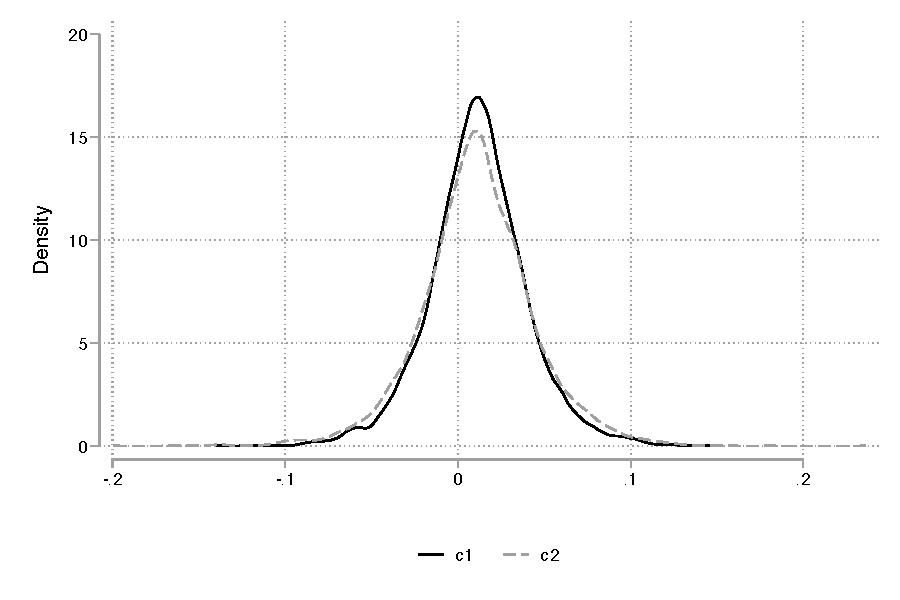
\includegraphics[width=0.7\textwidth]{figures/c1_c2_distr.pdf}\end{figure}
\end{center}

\begin{figure}[ptb]
  \caption{Relationship Between $c_{1}$ and $c_{2}$}%
  \label{fig:c1_c2}
  \centering
  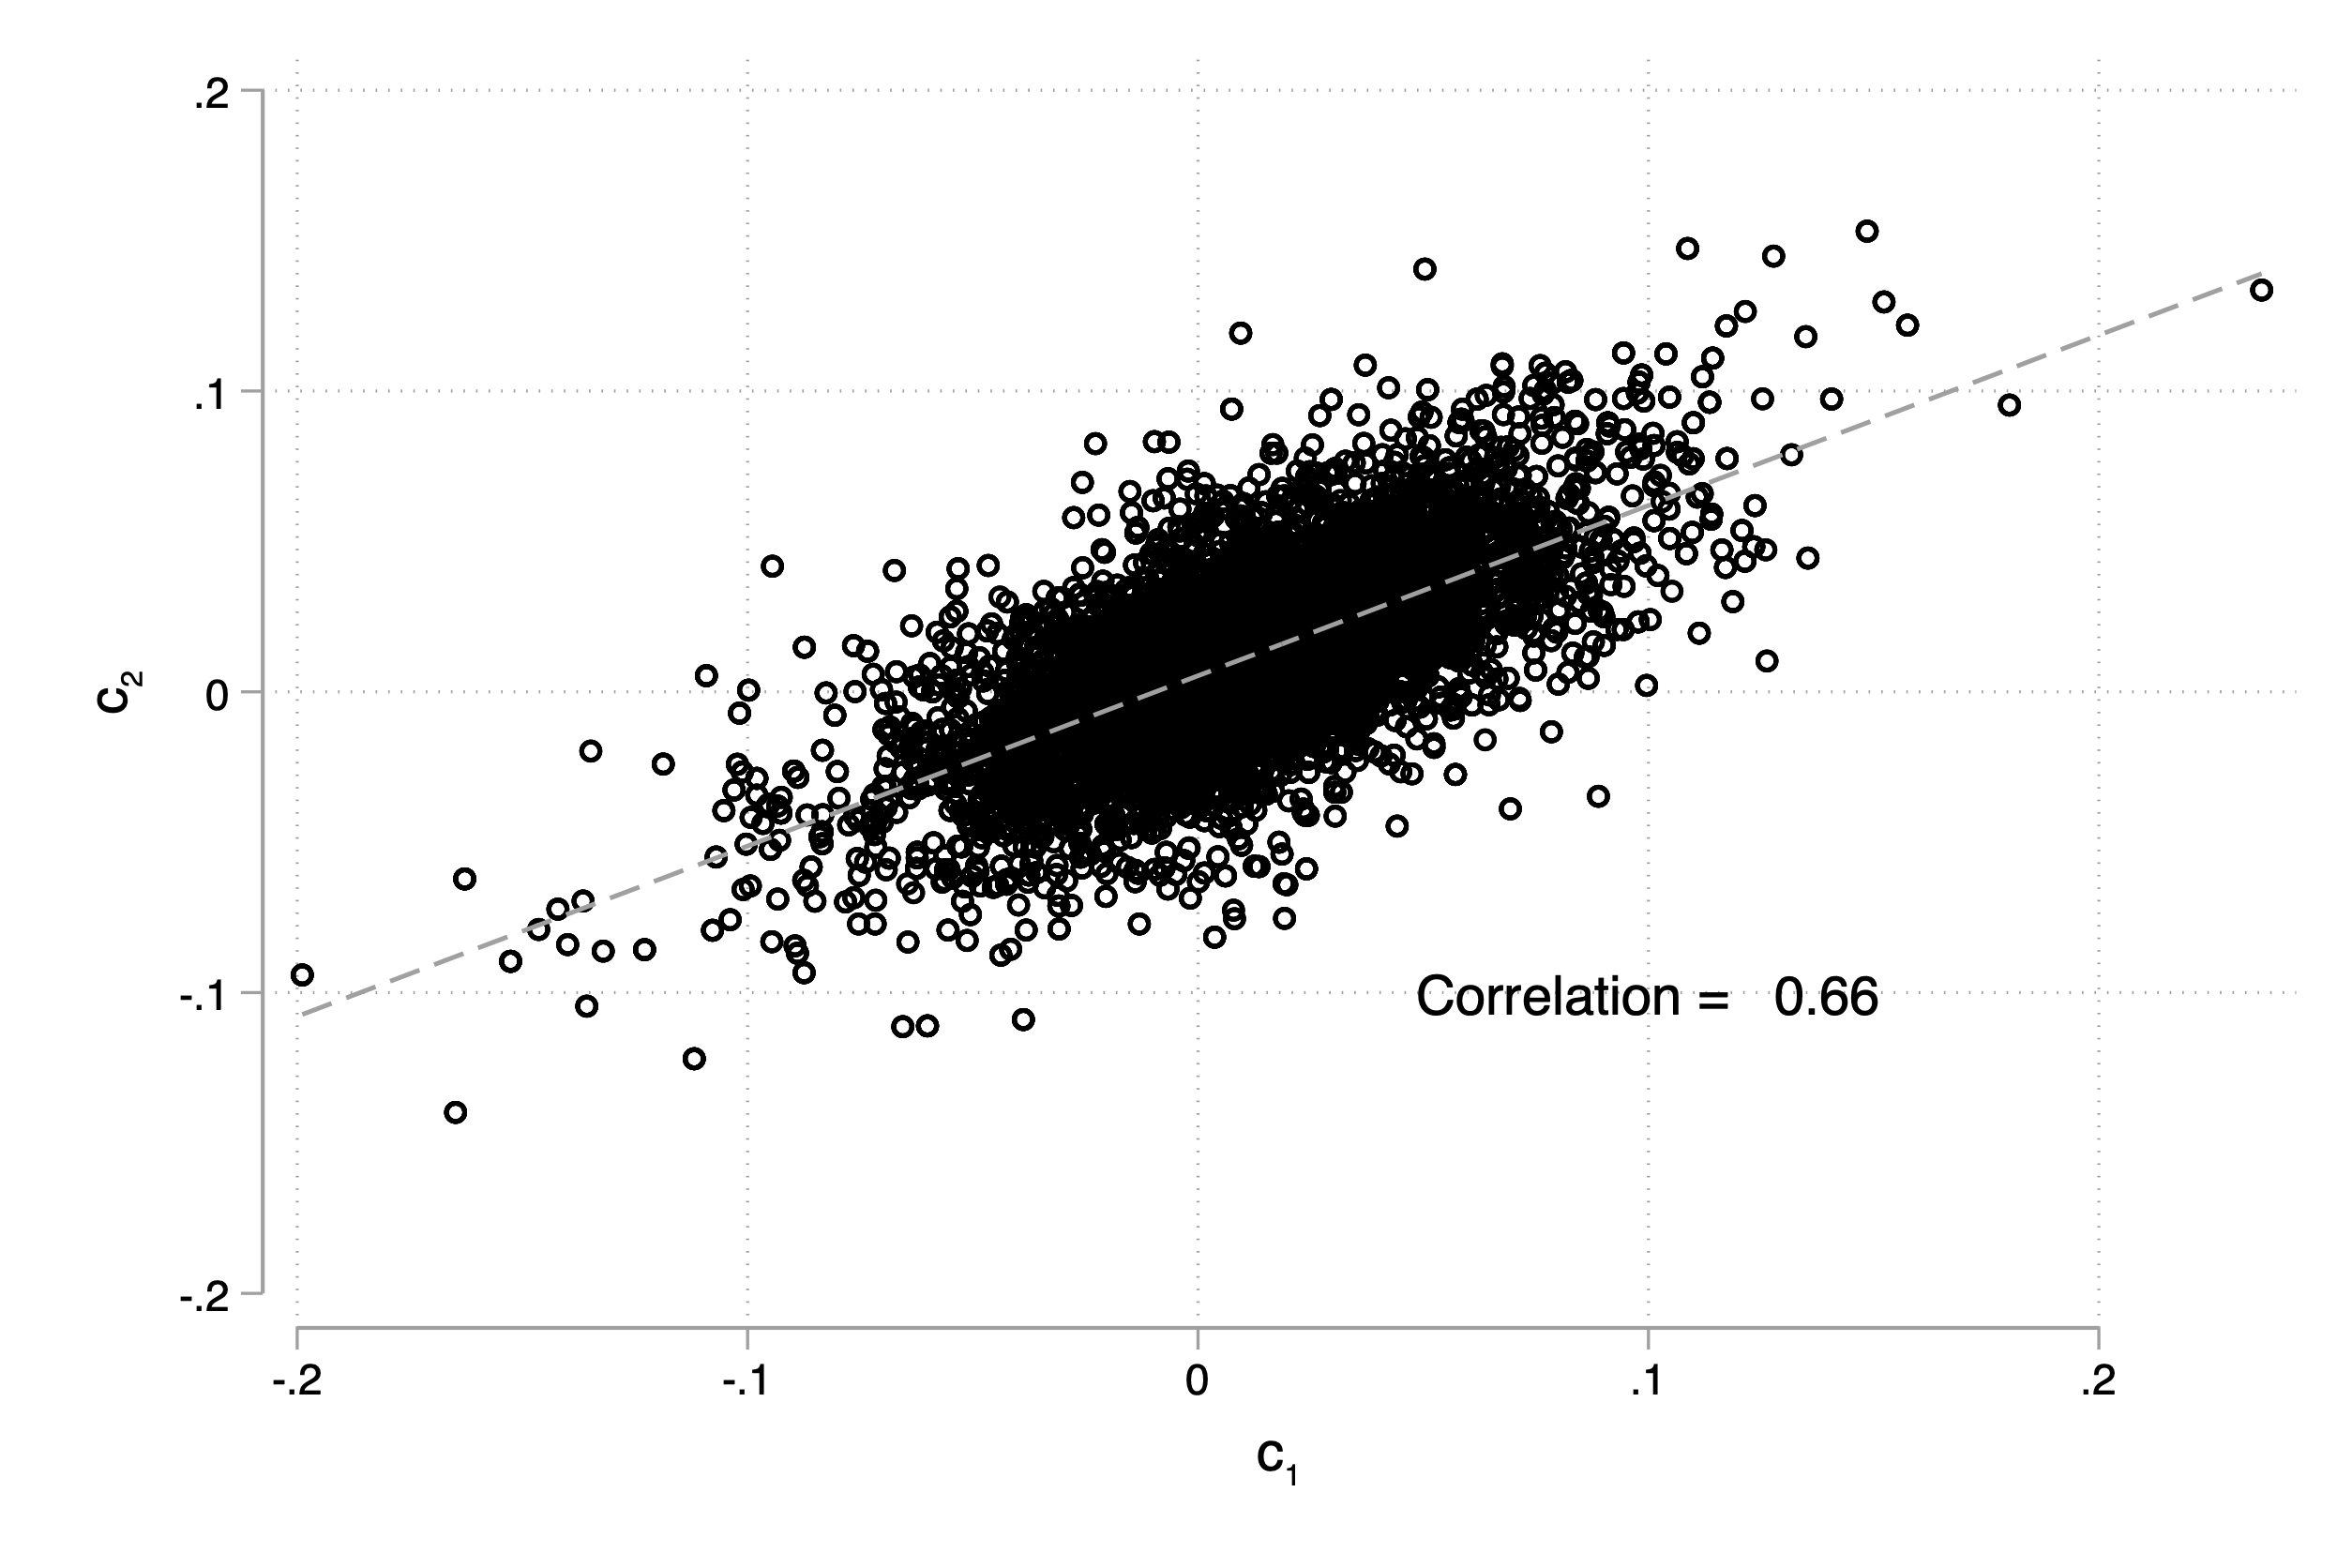
\includegraphics[width=0.8\textwidth]{figures/corr_c1_c2.png}\end{figure}\bigskip


\begin{figure}[ptb]
  \caption{Relationship Between $W_{d}^{0}\left(  x_{i}\right)  $ and
    $w_{it}^{0}$}
  \begin{center}
    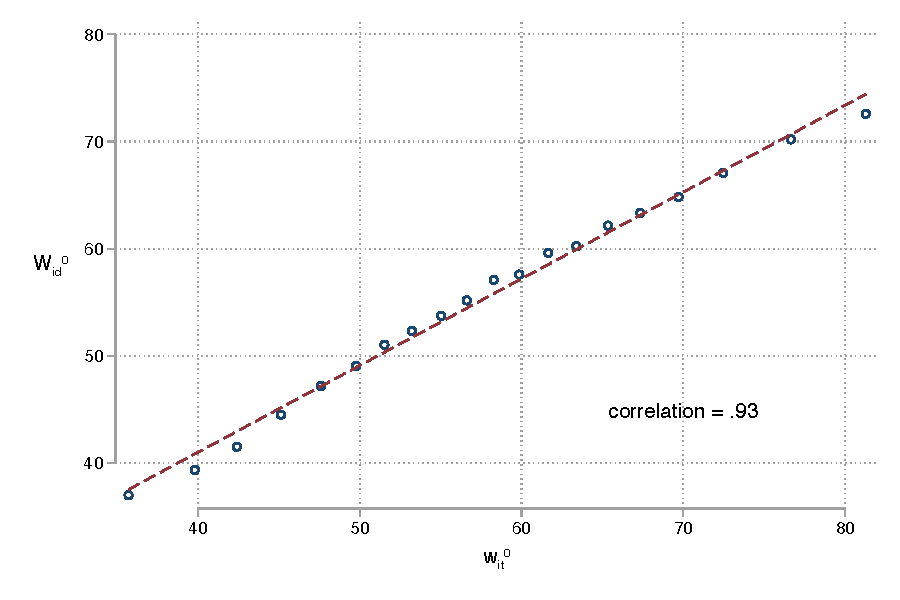
\includegraphics[width=0.6\textwidth]{figures/wage_schedule_pred.pdf}\newline%
    {\footnotesize {Note: Binned scatterplot of $W_{d}^{0}\left(  x_{i}\right)  $
        and $w_{it}^{0}$ using wage data from 2010.} }
  \end{center}
\end{figure}

\begin{figure}[ptb]
\caption{Relationship Between Deviations of True Wages from $w_{d}\left(
x,c|\omega\right)  $, obtained using rules $\left(  \ref{wrule}\right)  $ and
$\left(  \ref{wrule'}\right)  $}%
\label{omega23}
\begin{center}
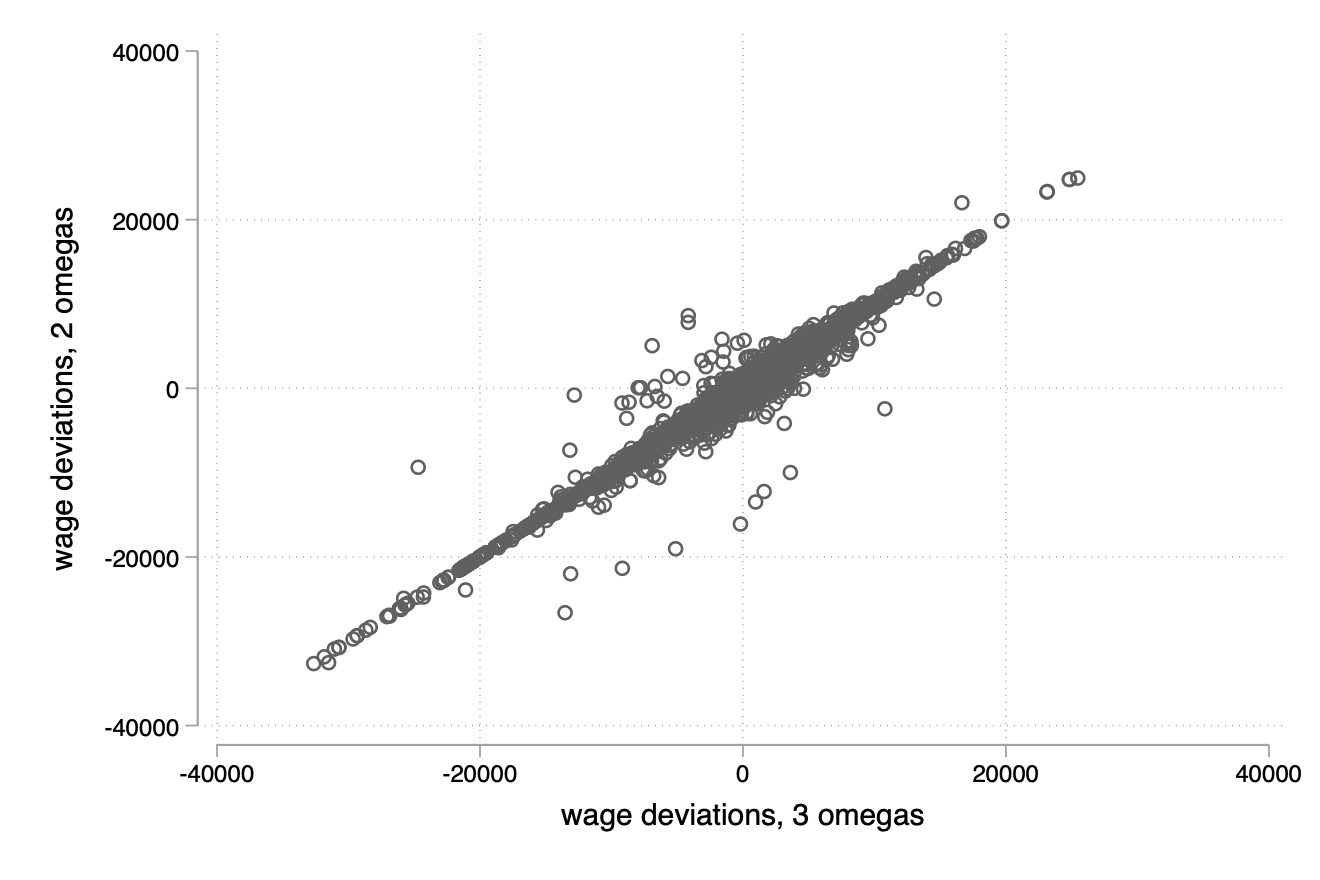
\includegraphics[width=0.8\textwidth]{figures/wagedeviations_3omega.png}\newline
\end{center}
\par
{\raggedleft {\footnotesize {Note: Binned scatterplot of the difference
between true 2014 teacher wages and $w_{d}\left(  x,c|\omega\right)  $,
calculated using $\left(  \ref{wrule} \right)  $ (vertical axis) and $\left(
\ref{wrule'} \right)  $ (horizontal axis). }}}\end{figure}

\begin{figure}[ptb]
\caption{Relationship Between Deviations of True Wages from $w_{d}\left(
x,c|\omega\right)  $, obtained using rules $\left(  \ref{wrule}\right)  $ and
$\left(  \ref{eq:wage_rob}\right)  $, where $x_{1}=1$ for untenured teachers}%
\label{wageresidual_untenured}
\begin{center}
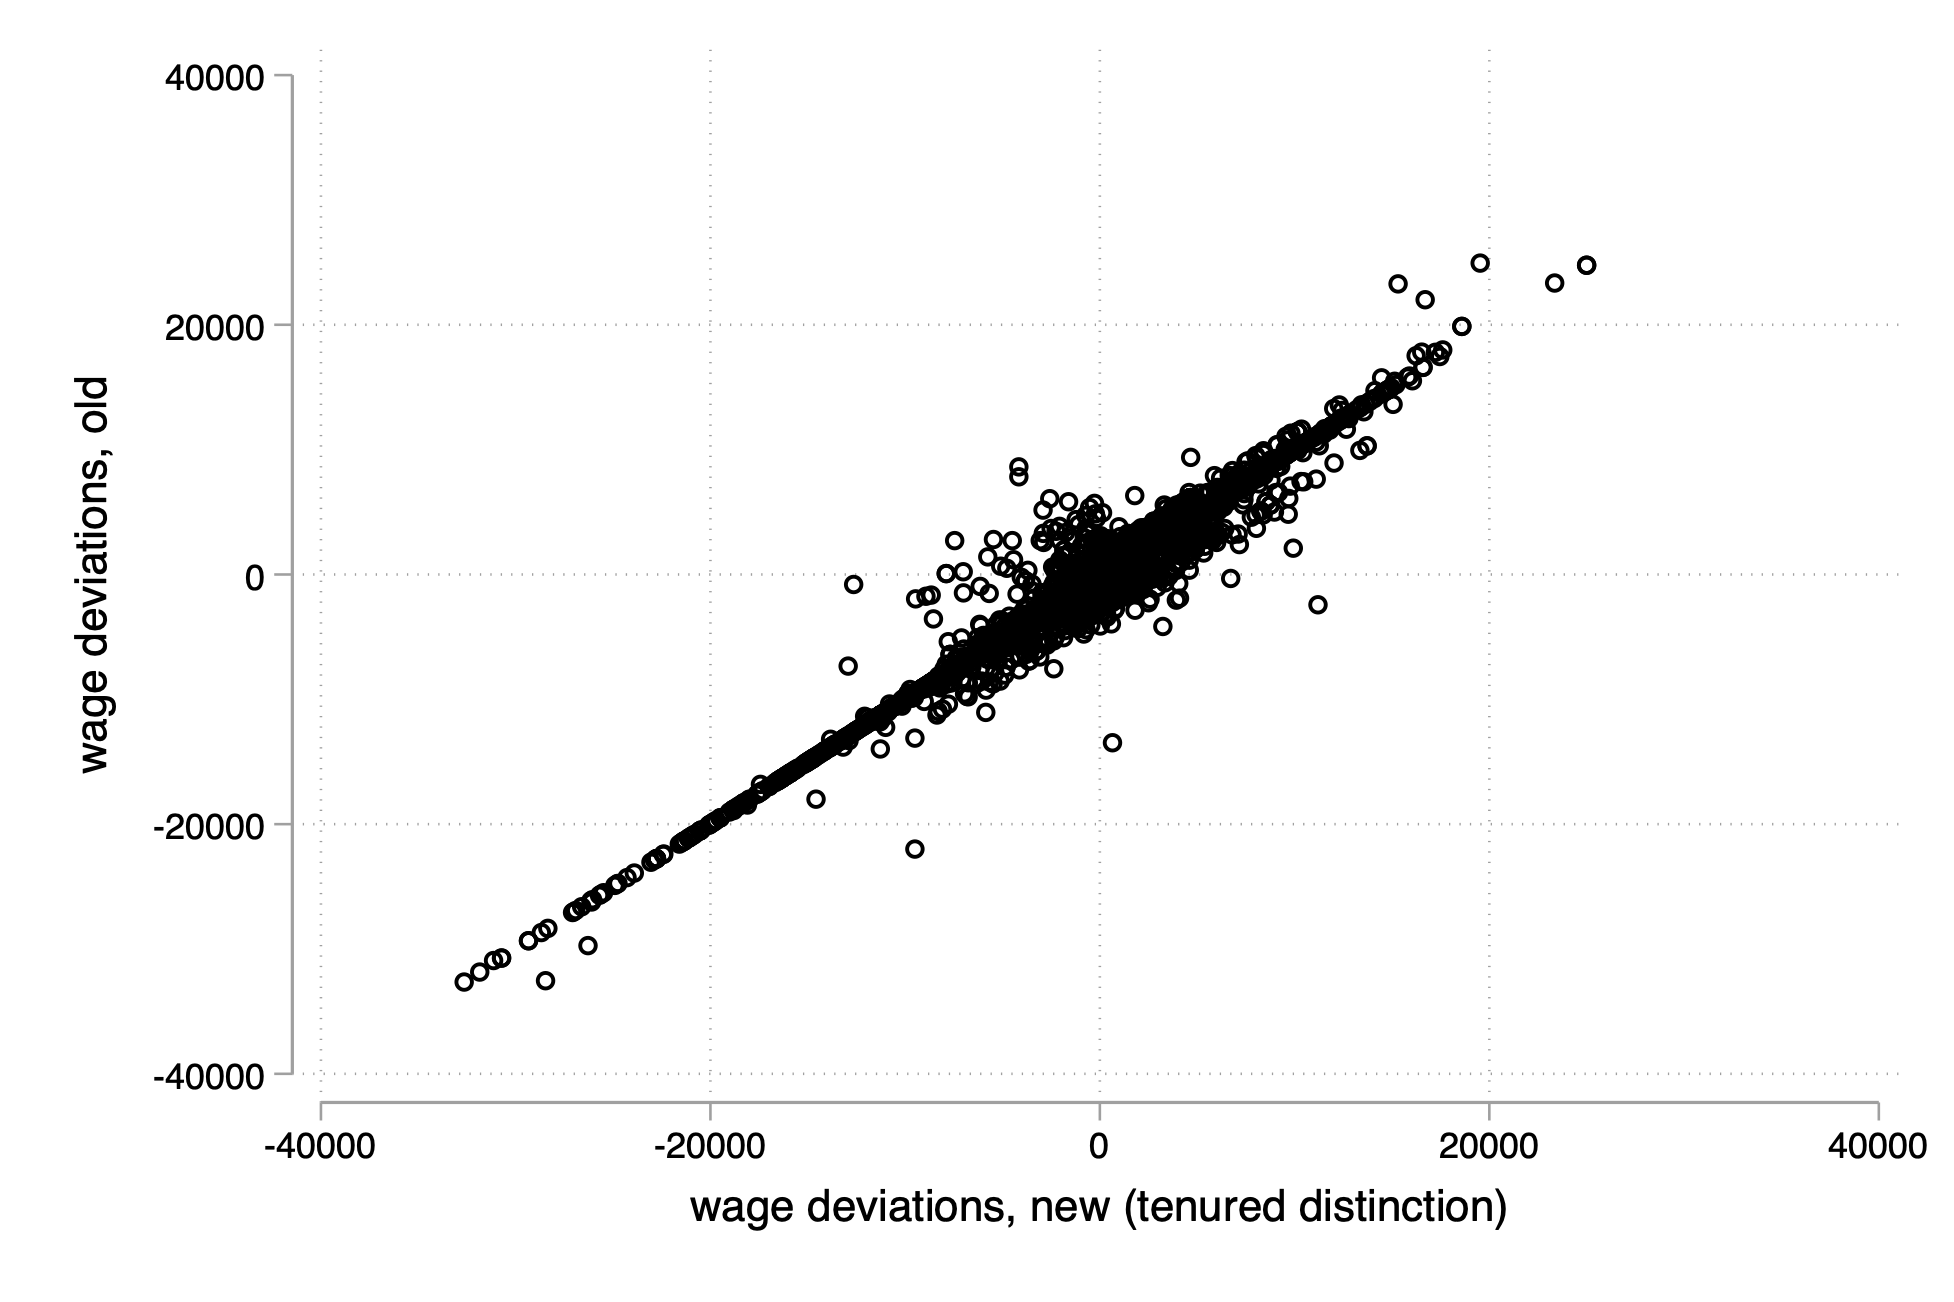
\includegraphics[width=0.8\textwidth]{figures/wagedeviations_tenured.png}
\end{center}
\par
{\raggedleft {\footnotesize {Note: Binned scatterplot of the difference
between true 2014 teacher wages and $w_{d}\left(  x,c|\omega\right)  $,
calculated using $\left(  \ref{wrule} \right)  $ (vertical axis) and $\left(
\ref{eq:wage_rob}\right)  $, where $x_{1}=1$ for untenured teachers
(horizontal axis). }}}\end{figure}

\begin{figure}[ptb]
\caption{{Relationship Between Deviations of True Wages from $w_{d}\left(
x,c|\omega\right)  $, obtained using rules $\left(  \ref{wrule}\right)  $ and
$\left(  \ref{eq:wage_rob}\right)  $, where $x_{1}=1$ for teachers with no
experience}}%
\label{wageresidual_exp1}
\begin{center}
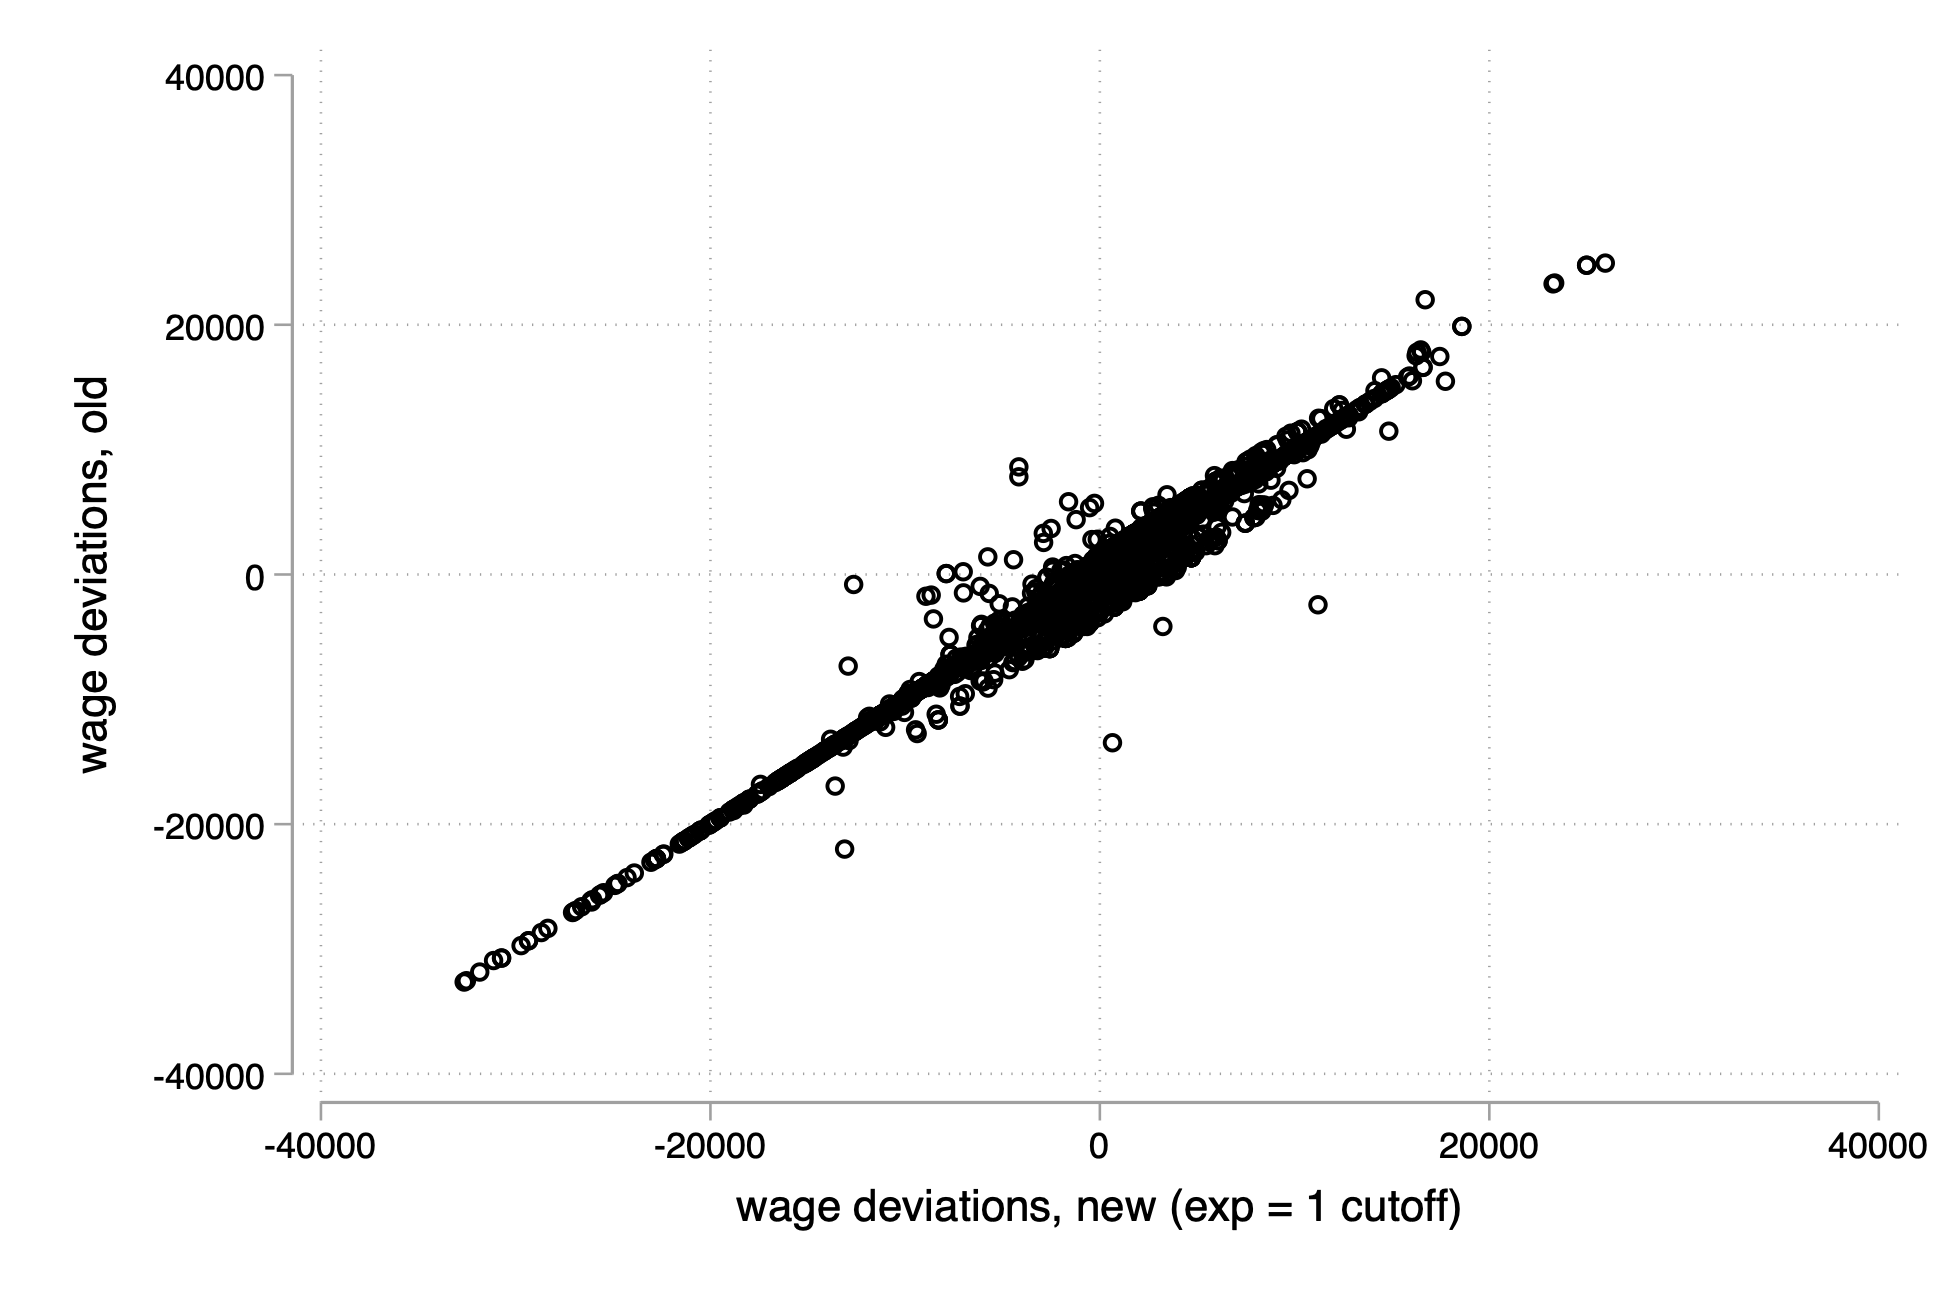
\includegraphics[width=0.8\textwidth]{figures/wagedeviations_exp1cutoff.png}\newline
\end{center}
\par
{\raggedleft {\footnotesize {Note: Binned scatterplot of the difference
between true 2014 teacher wages and $w_{d}\left(  x,c|\omega\right)  $,
calculated using $\left(  \ref{wrule} \right)  $ (vertical axis) and $\left(
\ref{eq:wage_rob}\right)  $, where $x_{1}=1$ for teachers with no experience
(horizontal axis). }}}\end{figure}

\begin{figure}[ptb]
\caption{Share of Teachers Who Switch In and Out of Math Teaching, By Year}%
\label{fig:match_switch}
\begin{center}
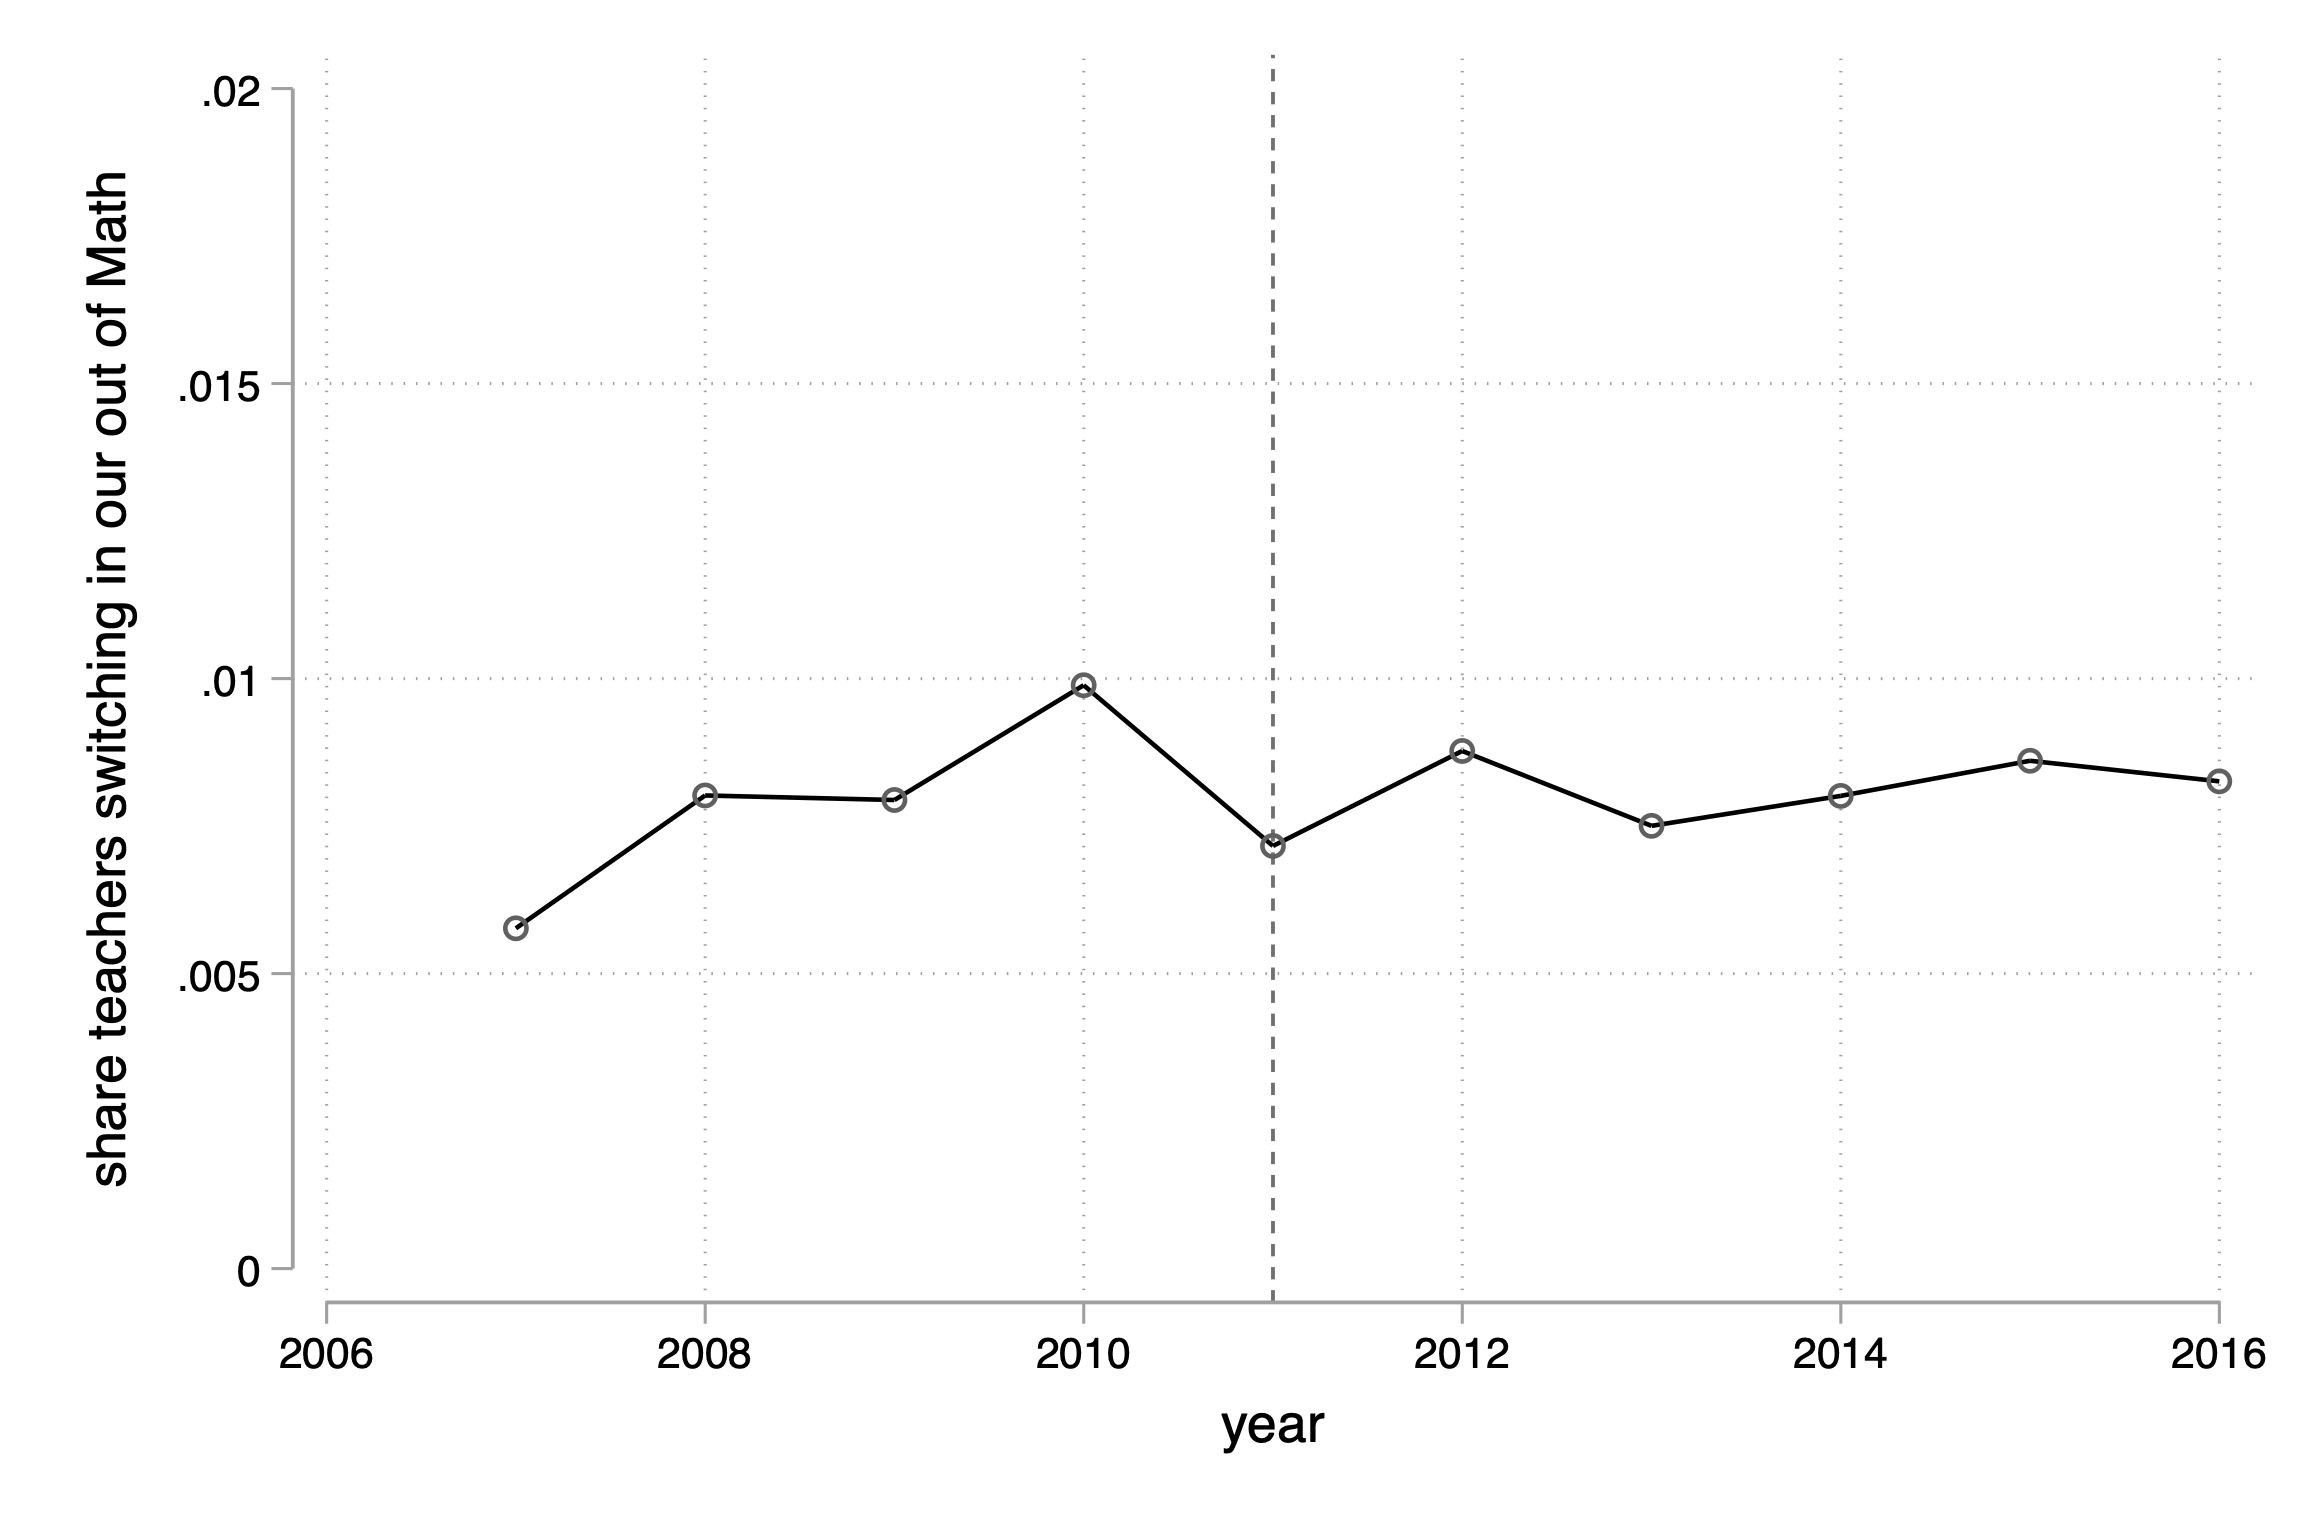
\includegraphics[width=0.8\textwidth]{figures/math_switch}
\end{center}
\par
{\raggedleft {\footnotesize {Note: Share of teachers who switch into or out of
math teaching, in each year and out of the total number of teachers in
Wisconsin.} }}\end{figure}

\begin{figure}[ptb]
\caption{Share of Districts' Budgets Spent on Teacher Salaries, by Grade and
Subject}%
\label{fig:budget}
\begin{subfigure}{0.49\textwidth}
\caption{Math, Grades 4-6}
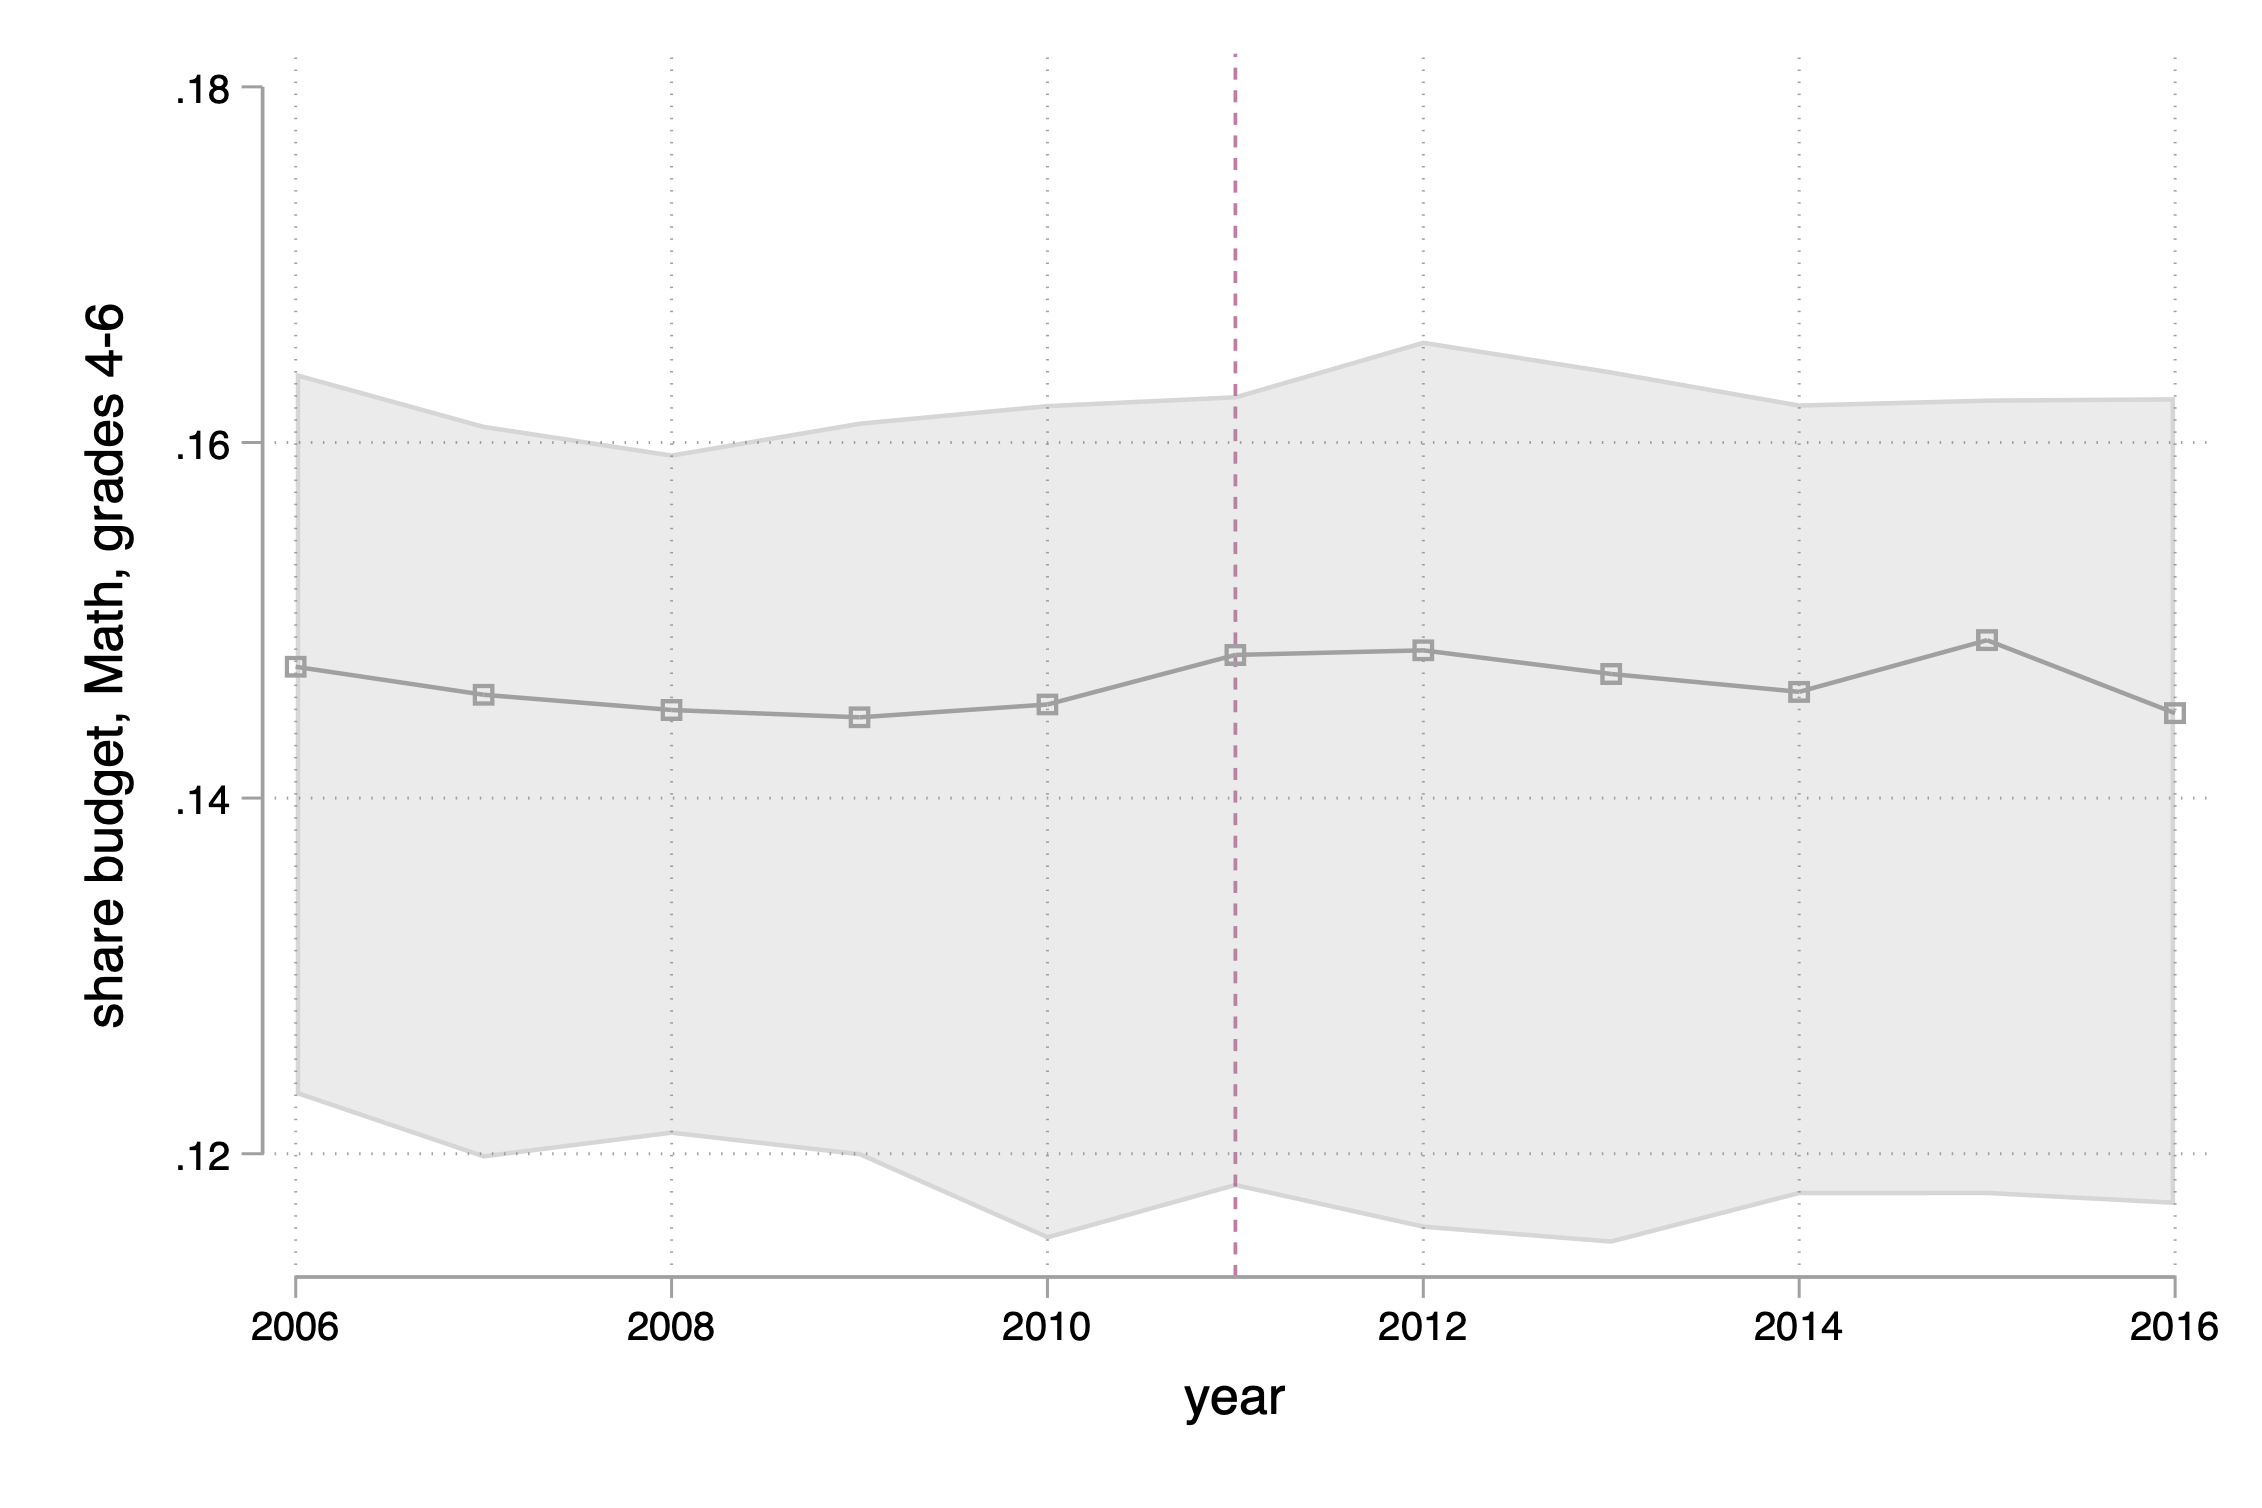
\includegraphics[width=\textwidth]{figures/budget_allocated_math}
\end{subfigure}
\begin{subfigure}{0.49\textwidth}
\caption{Reading/ELA, Grades 4-6}
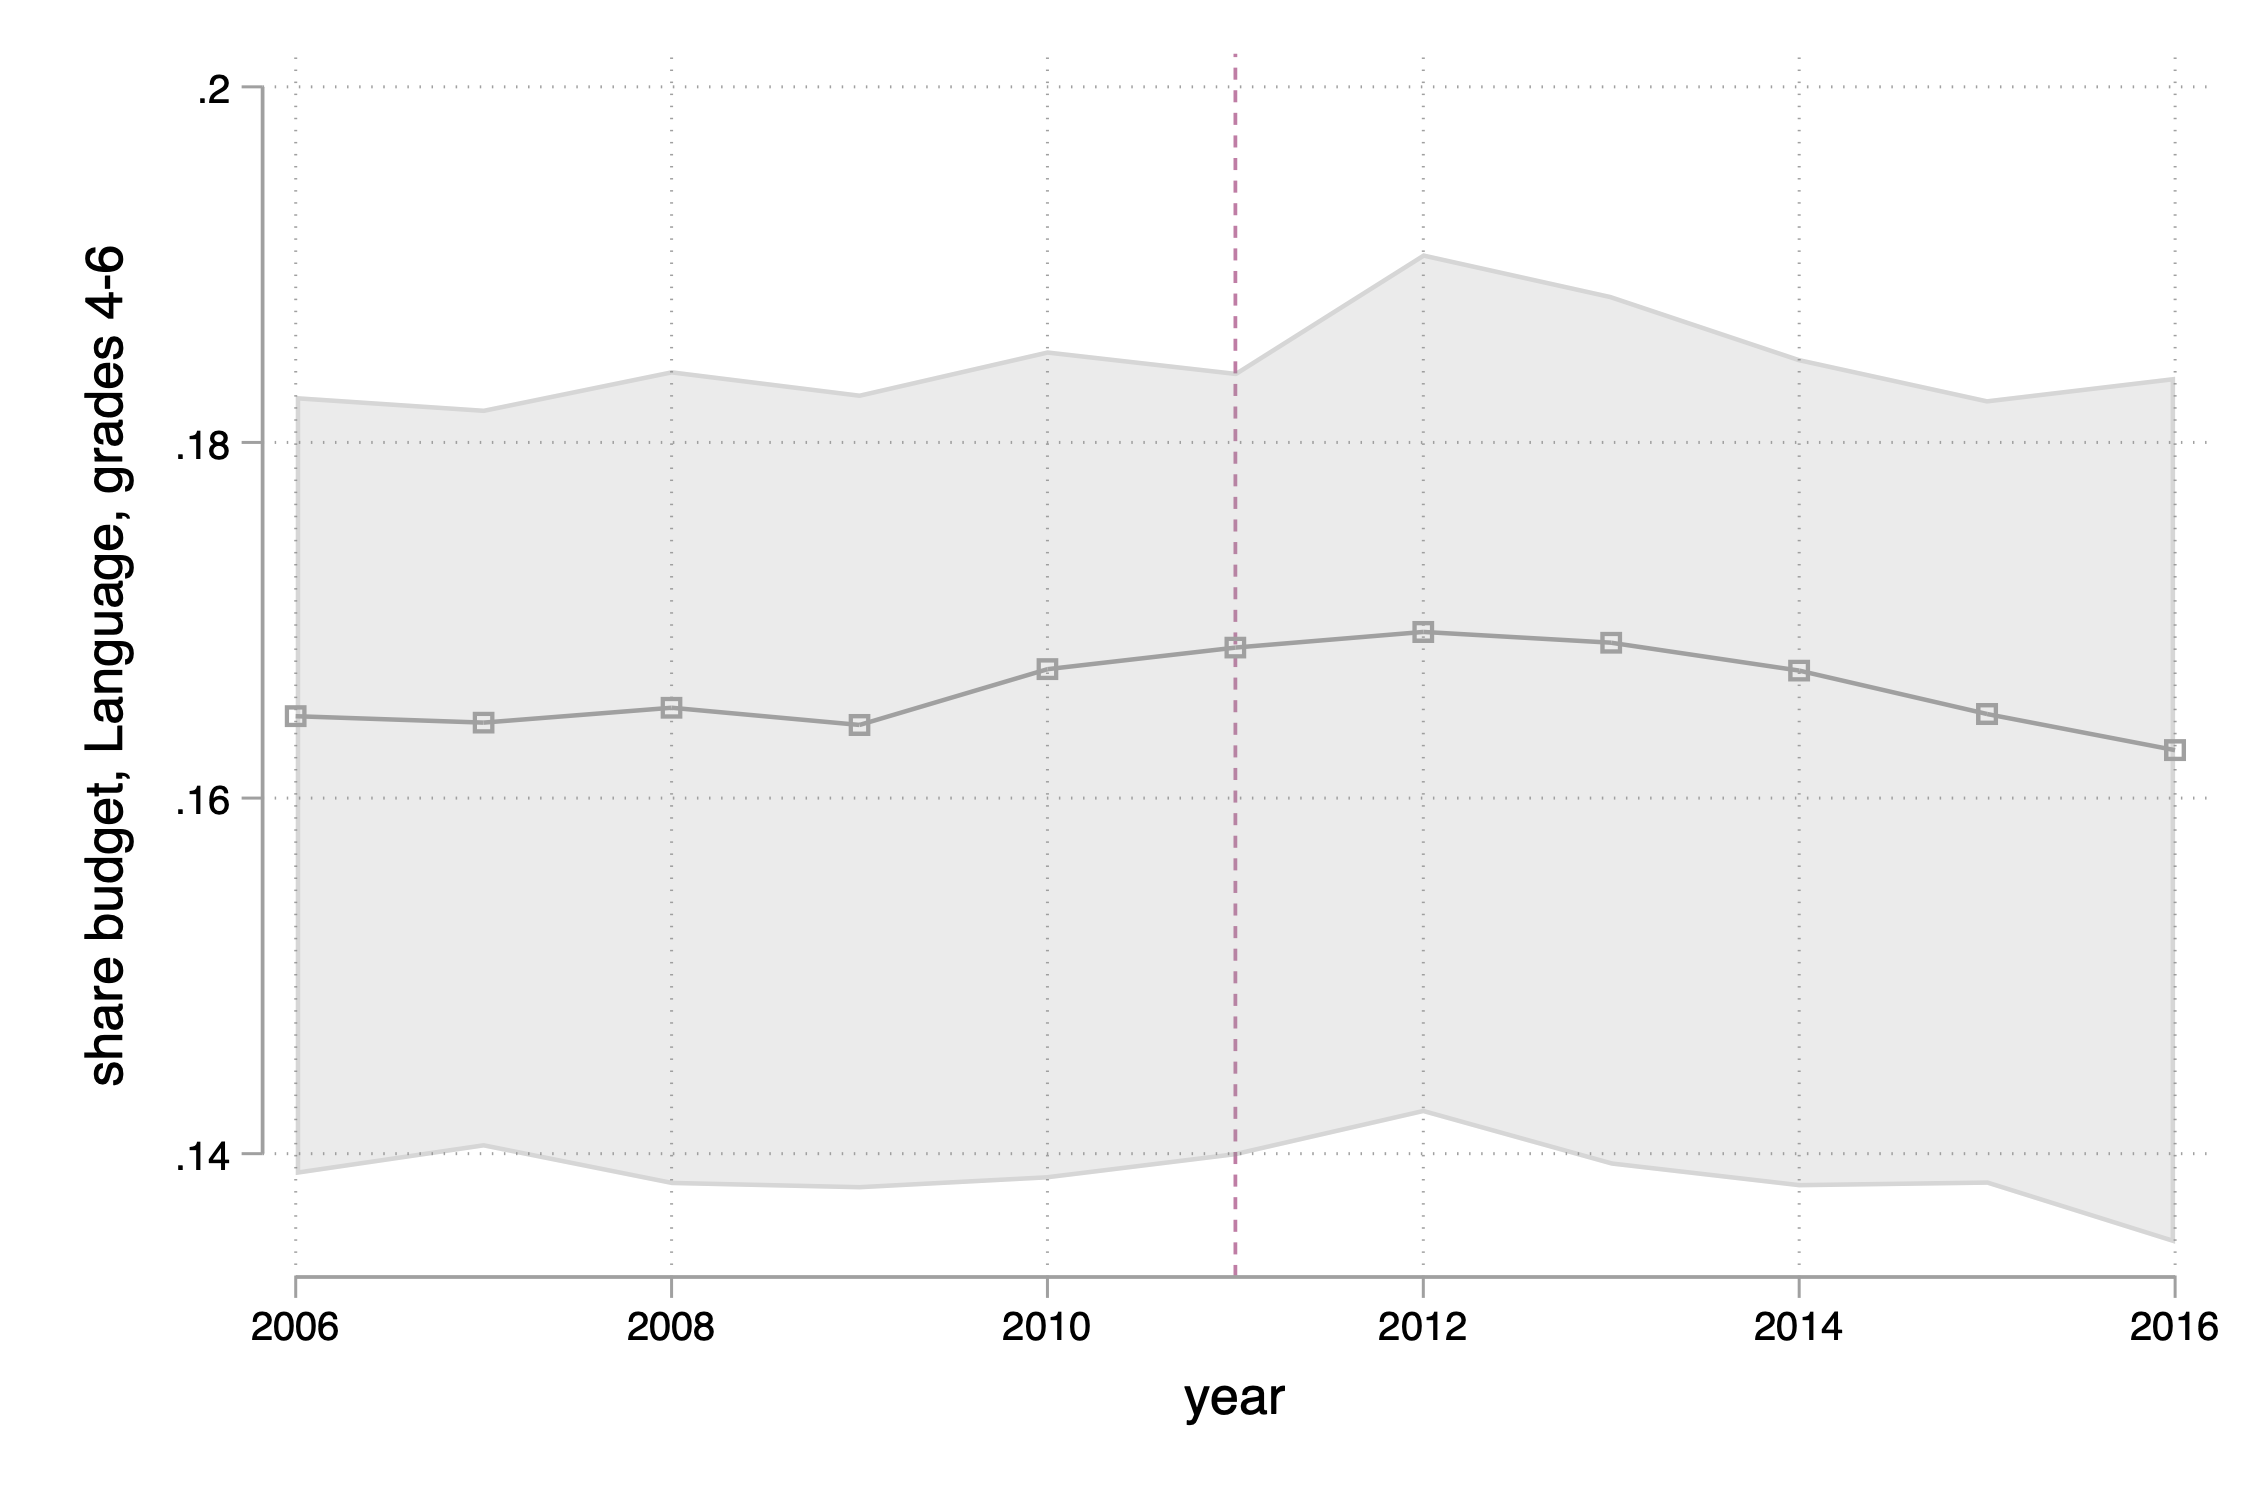
\includegraphics[width=\textwidth]{figures/budget_allocated_lang}
\end{subfigure}
\begin{subfigure}{0.49\textwidth}
\caption{All Teachers, Grades 4-6}
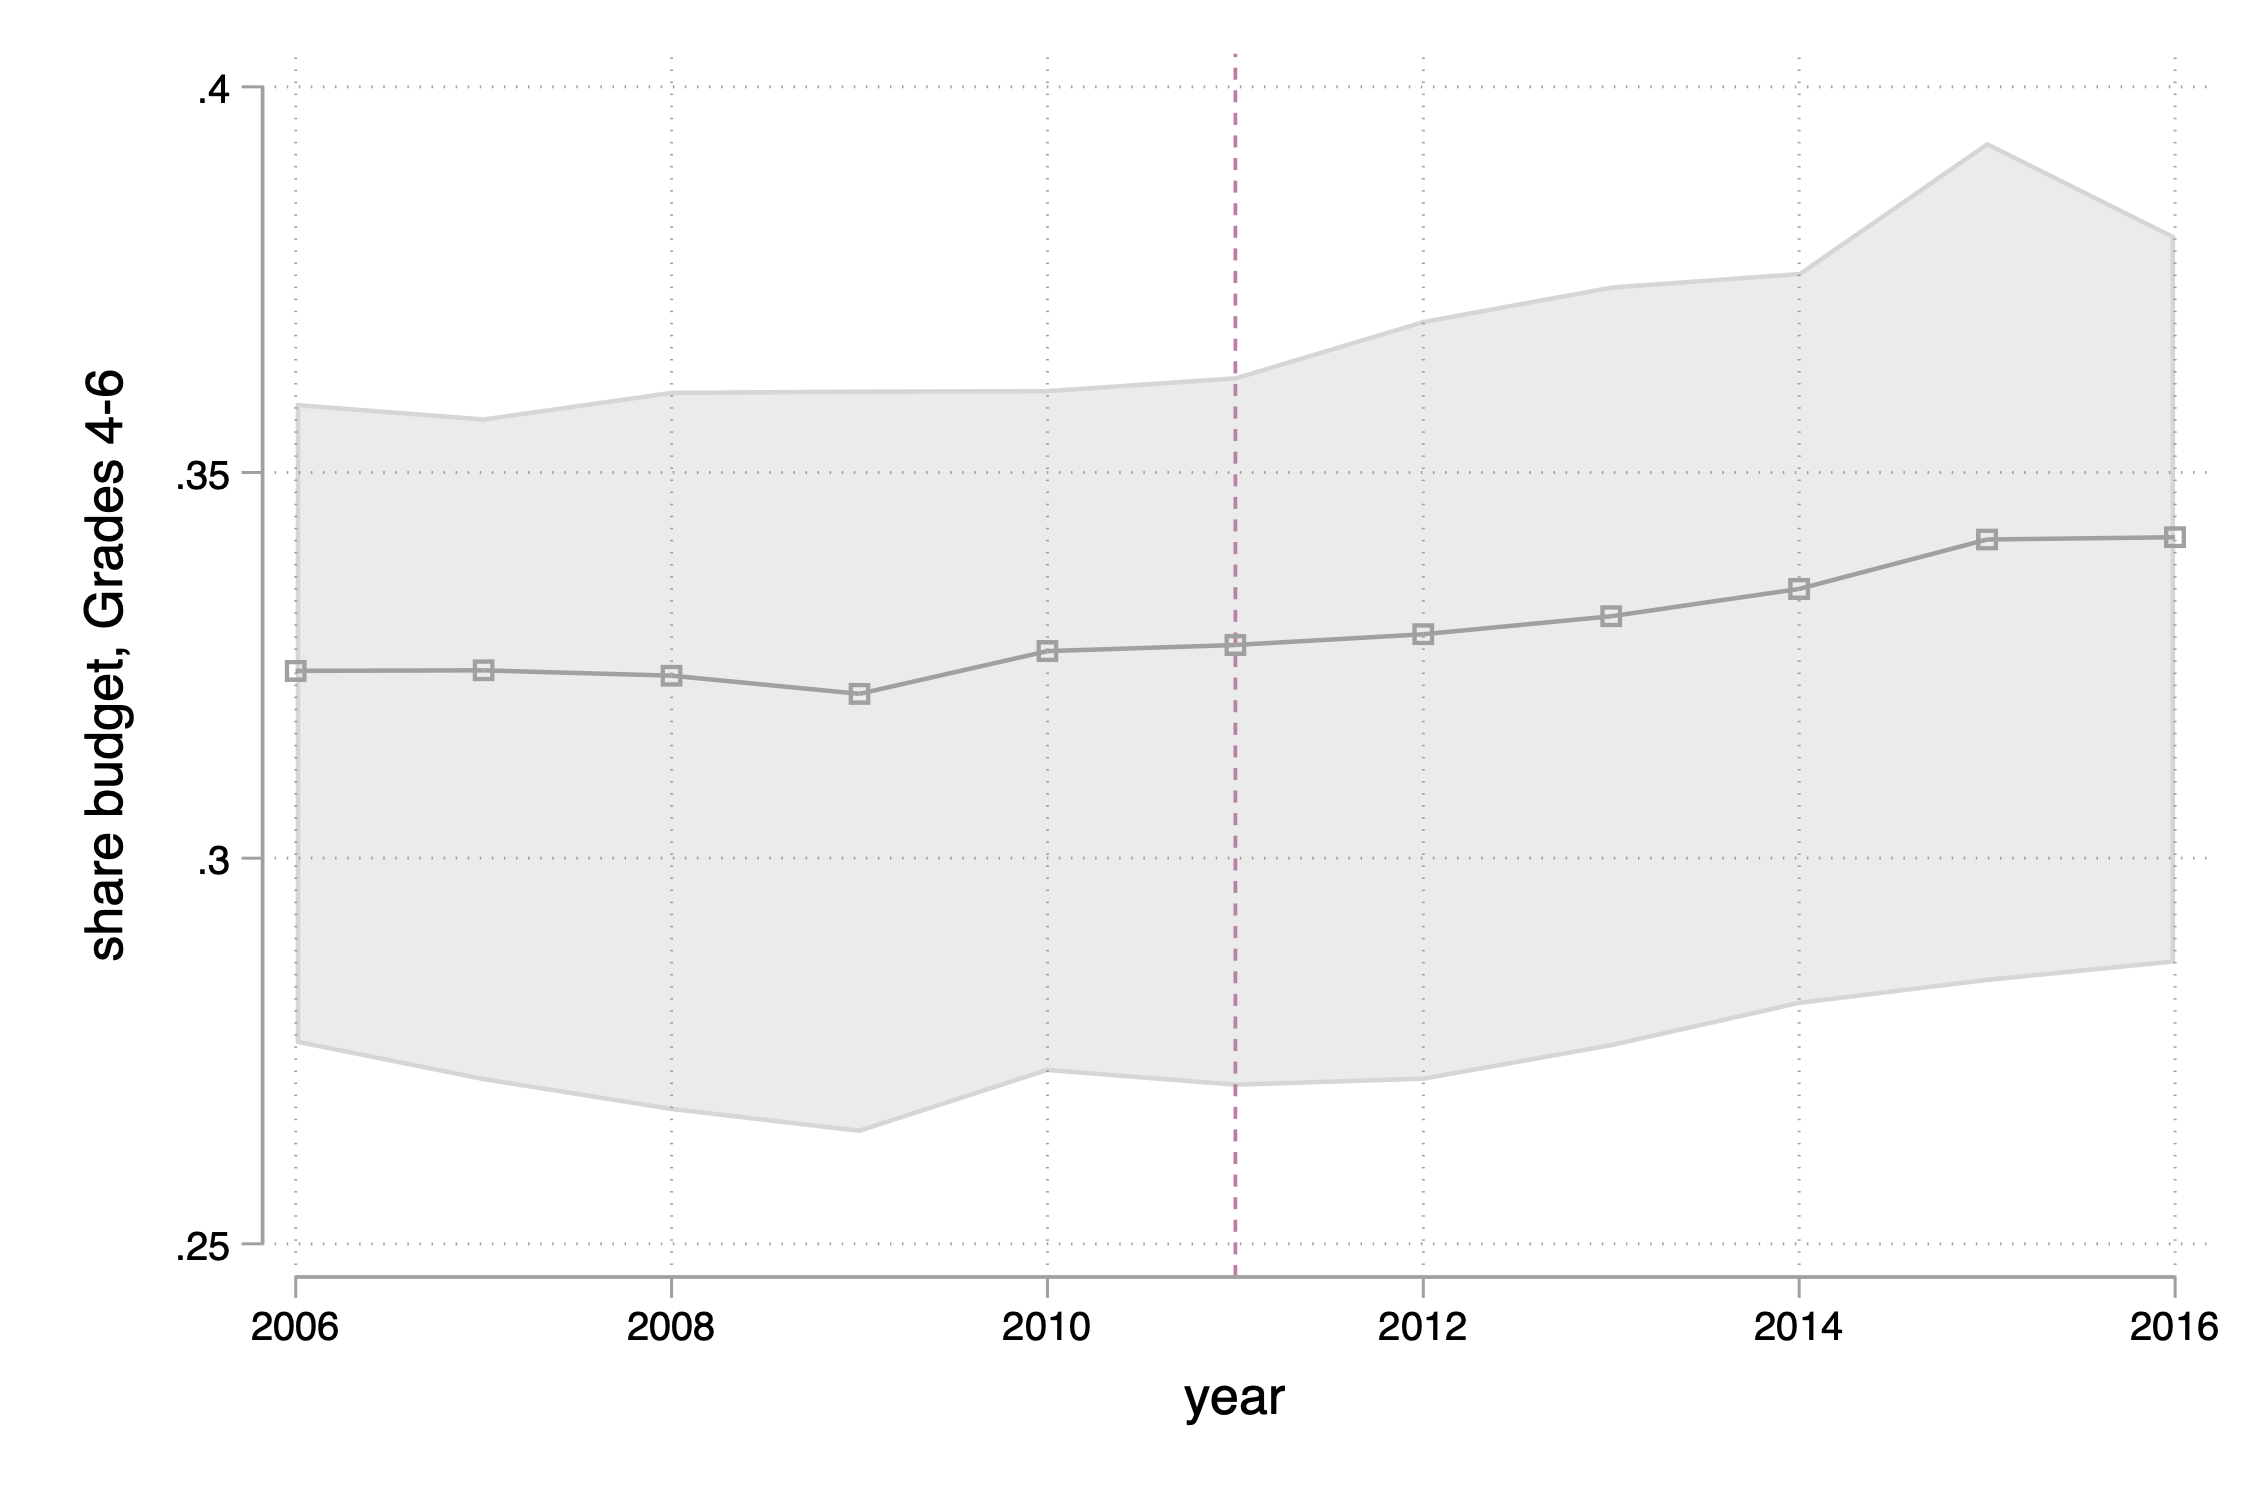
\includegraphics[width=\textwidth]{figures/budget_allocated_grades_4_6}
\end{subfigure}
\begin{subfigure}{0.49\textwidth}
\caption{All Teachers, Grades 1-3}
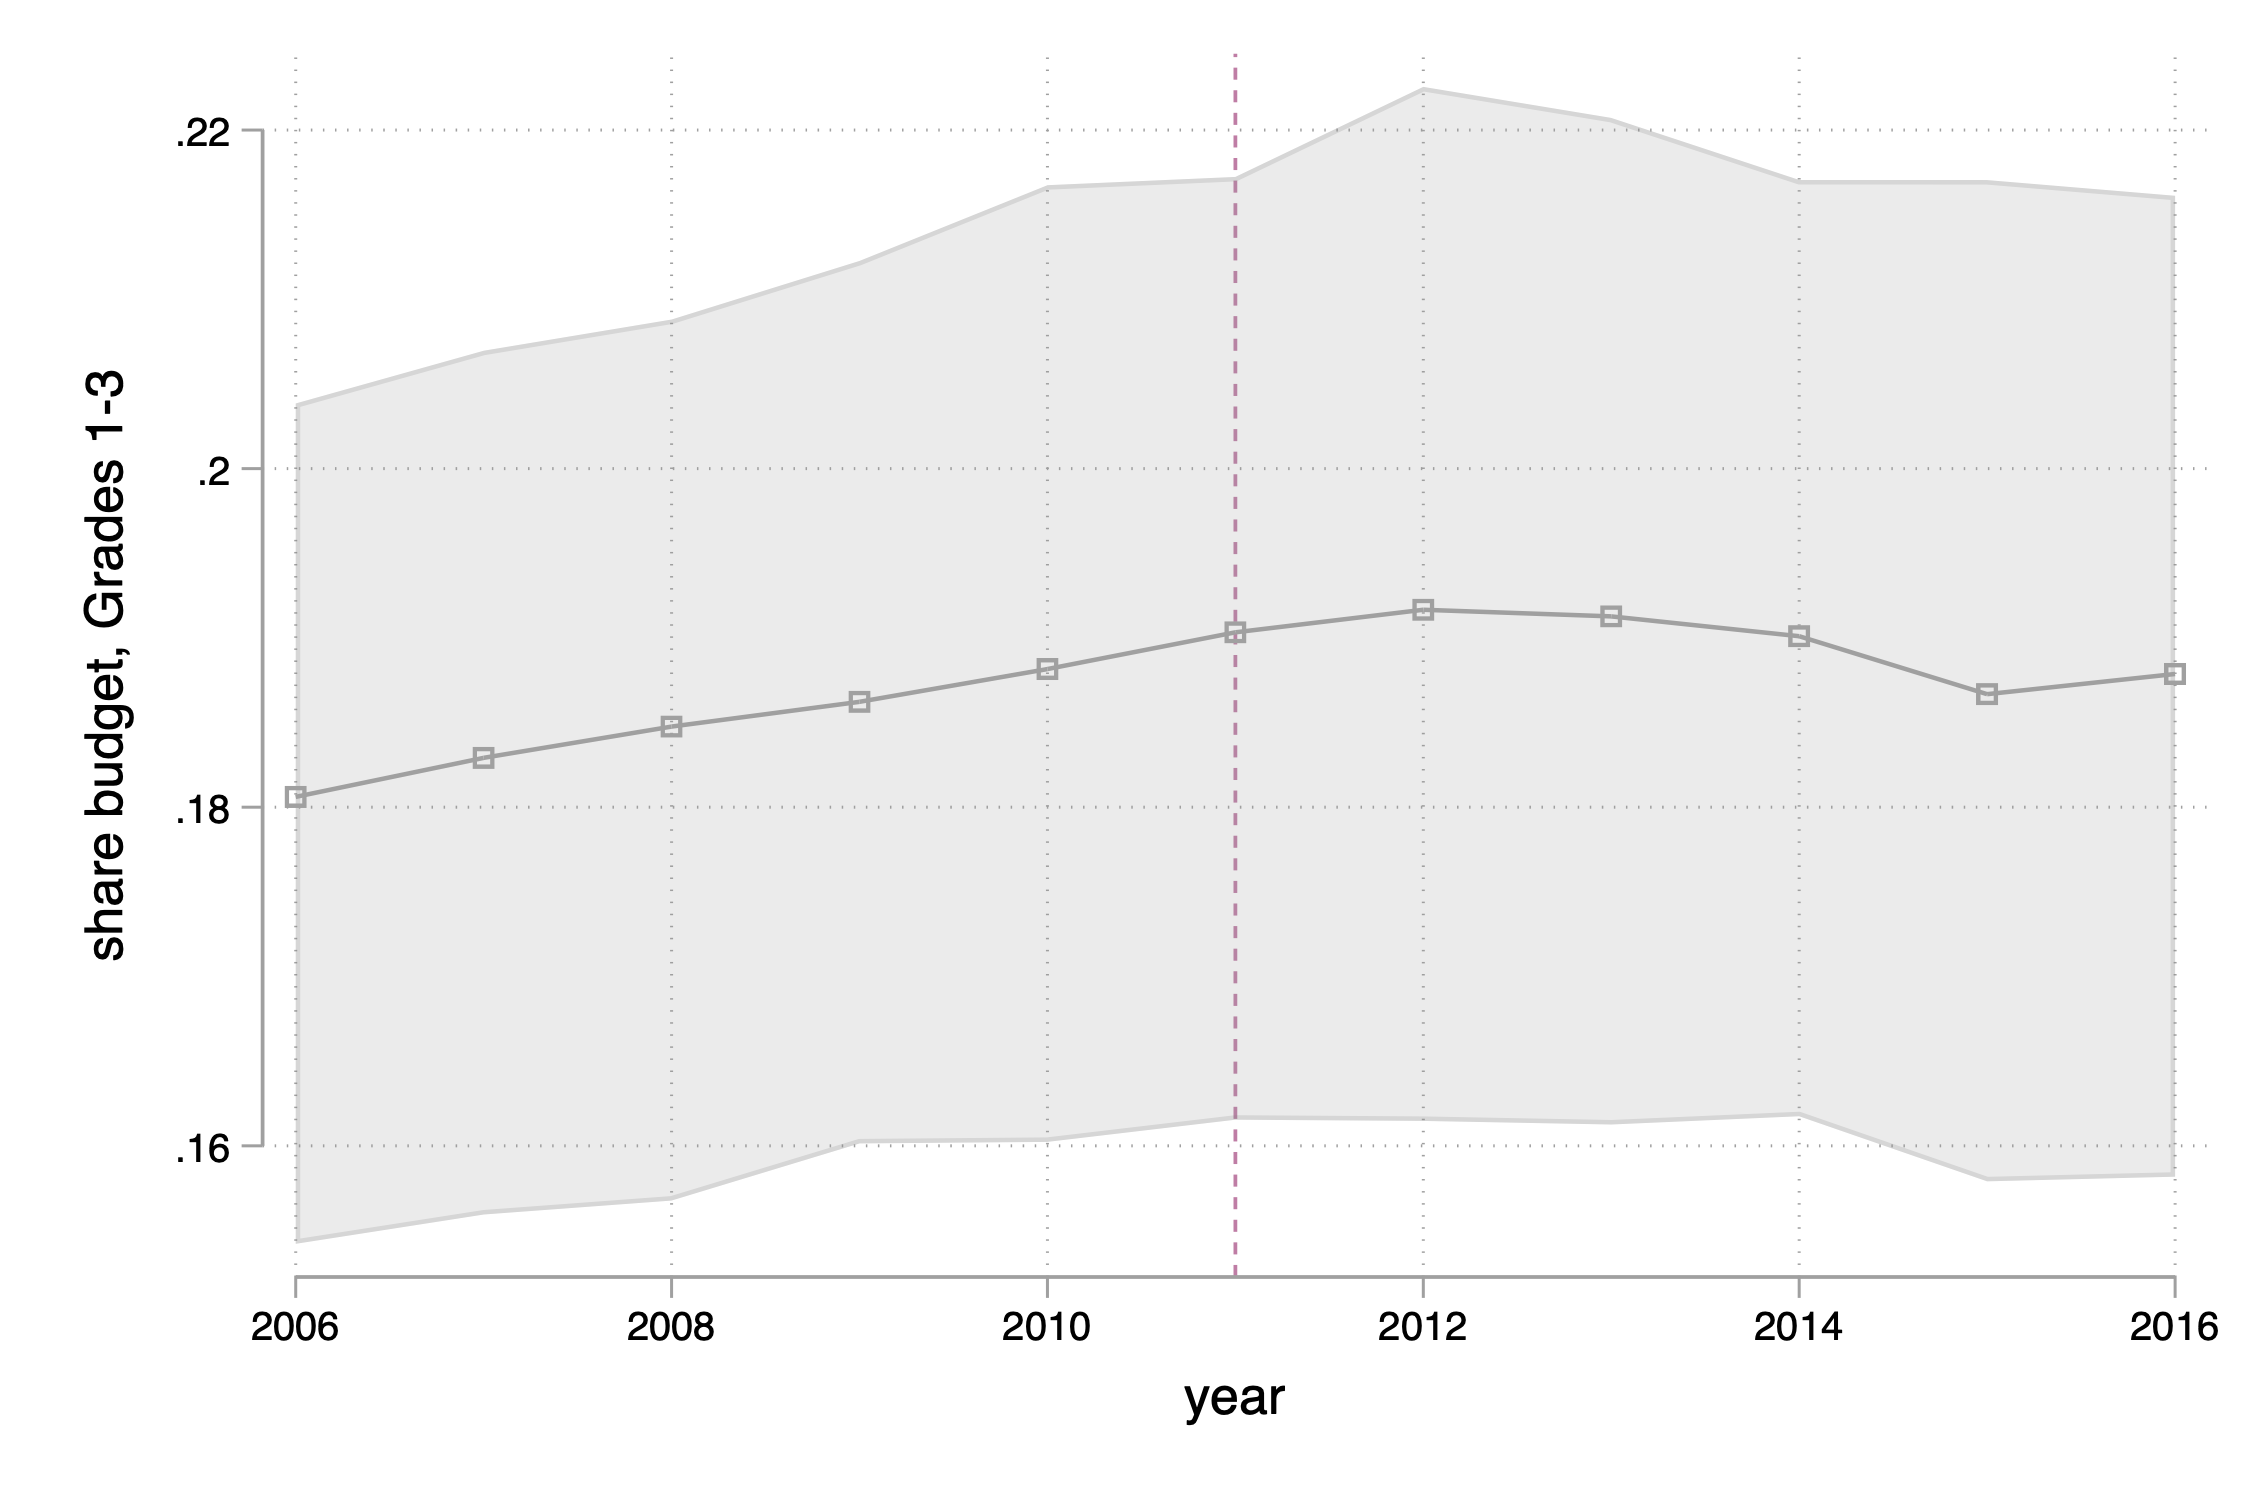
\includegraphics[width=\textwidth]{figures/budget_allocated_grades_1_3}
\end{subfigure}
{\footnotesize Notes: The figure shows the mean and the interquartile range of
the share of total wages paid to teachers in each subgroup, calculated for
each district. }\end{figure}

\begin{figure}[ptb]
  \caption{Identification Illustrated}
  \label{fig:b_02_1_5}%
  \centering
  \begin{subfigure}[t]{0.45\textwidth}
    \centering
    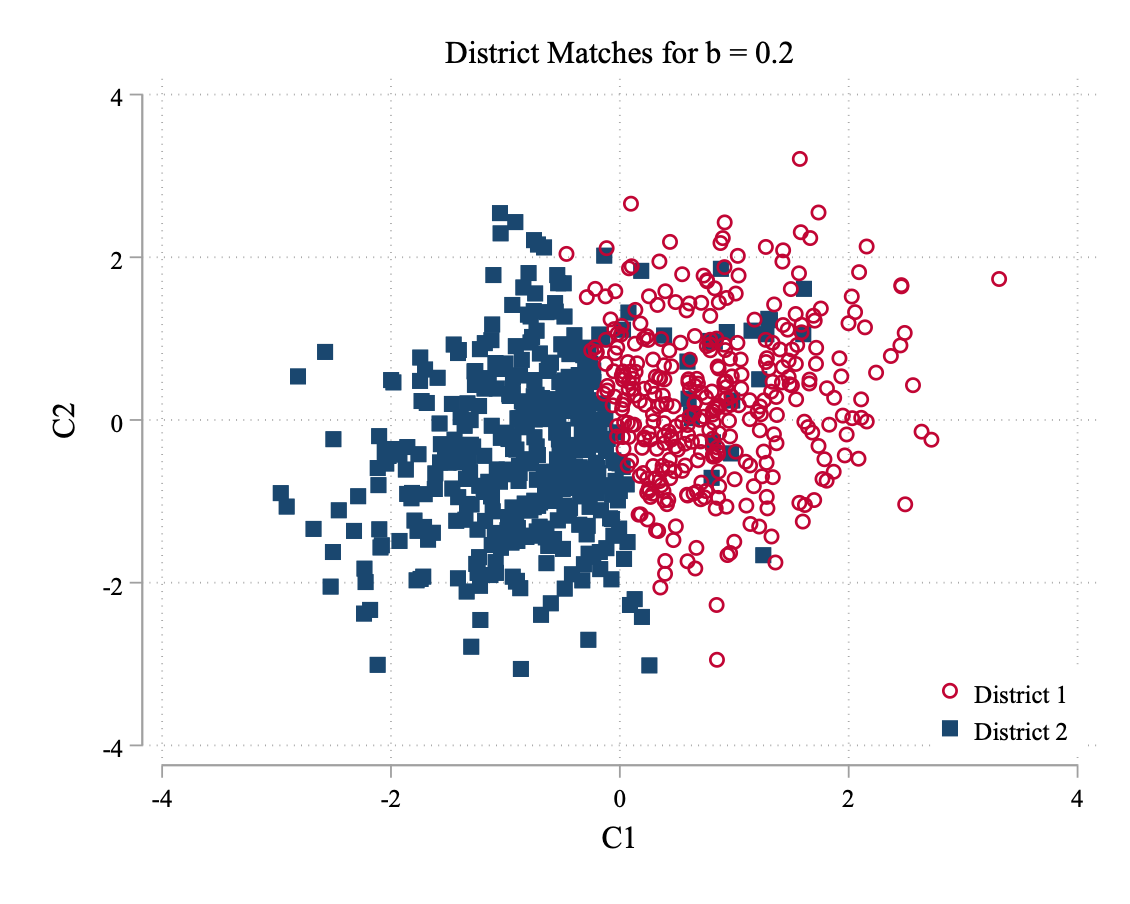
\includegraphics[width=\linewidth]{figures/b_02.png}
    \caption{} \label{fig:b_02}
  \end{subfigure}
  \hfill\begin{subfigure}[t]{0.45\textwidth}
    \centering
    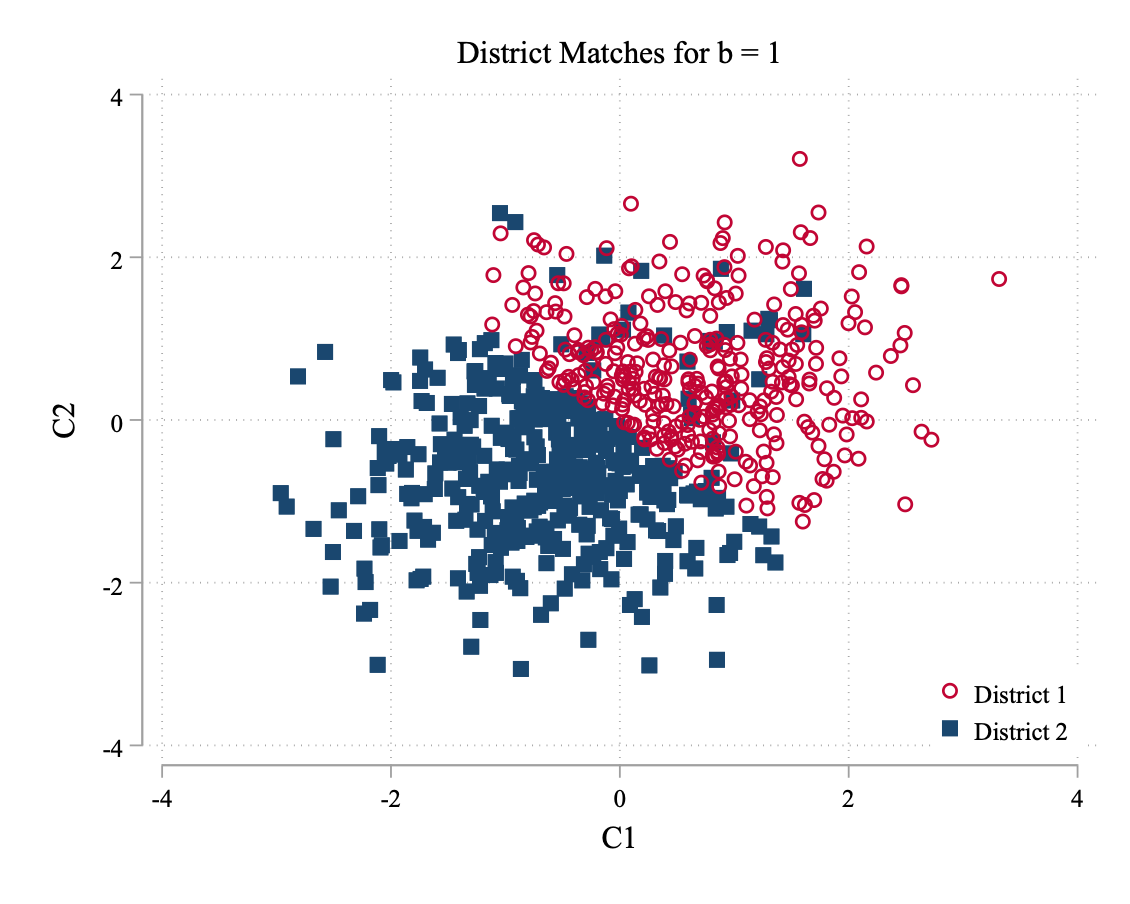
\includegraphics[width=\linewidth]{figures/b_1.png}
    \caption{} \label{fig:b_1}
  \end{subfigure}
  \par
  \vspace{1cm} \begin{subfigure}[t]{0.45\textwidth}
    \centering
    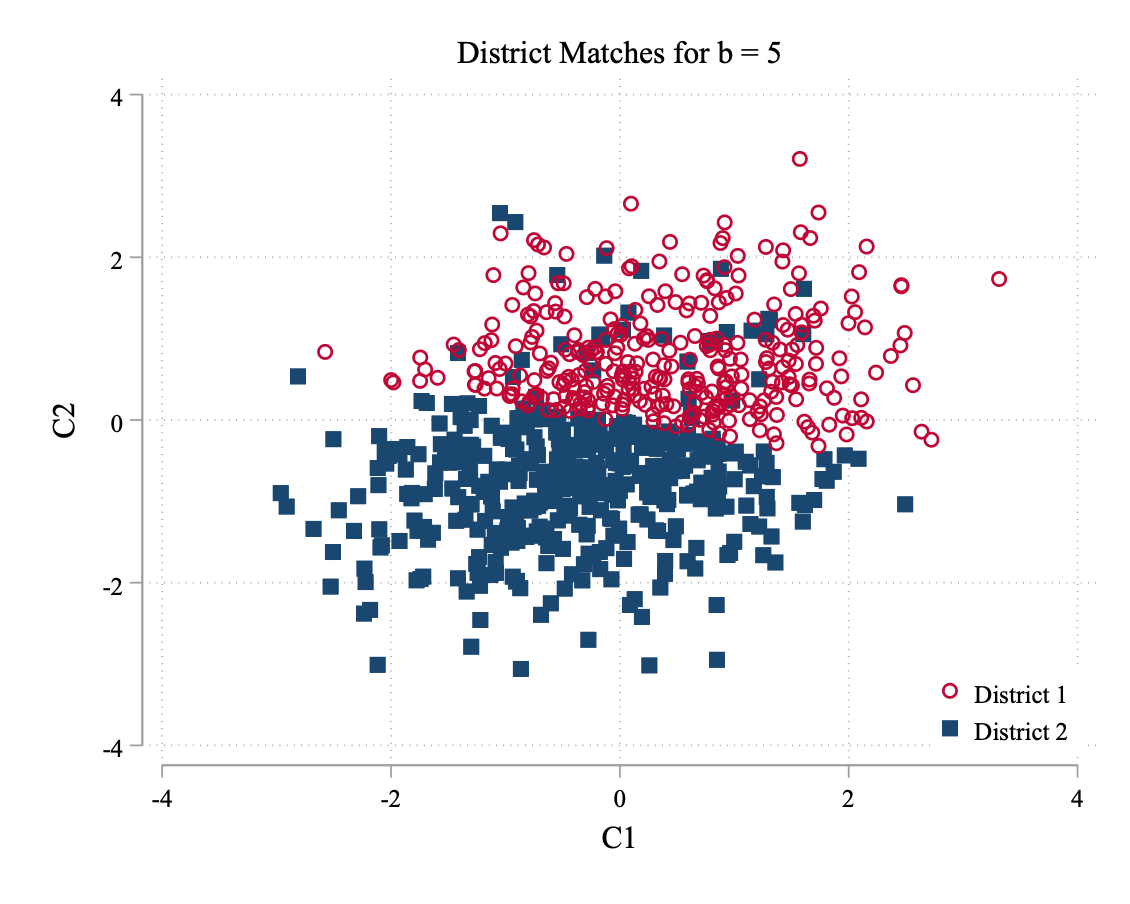
\includegraphics[width=\linewidth]{figures/b_5.png}
    \caption{} \label{fig:b_5}
  \end{subfigure}\\
  {\footnotesize Notes: These figures show the results of our simple example to illustrate identification; see B4.3 for details.}
\end{figure}

\begin{figure}
  \caption{Distribution of $\lambda$ Across Wisconsin Districts}
  \centering
  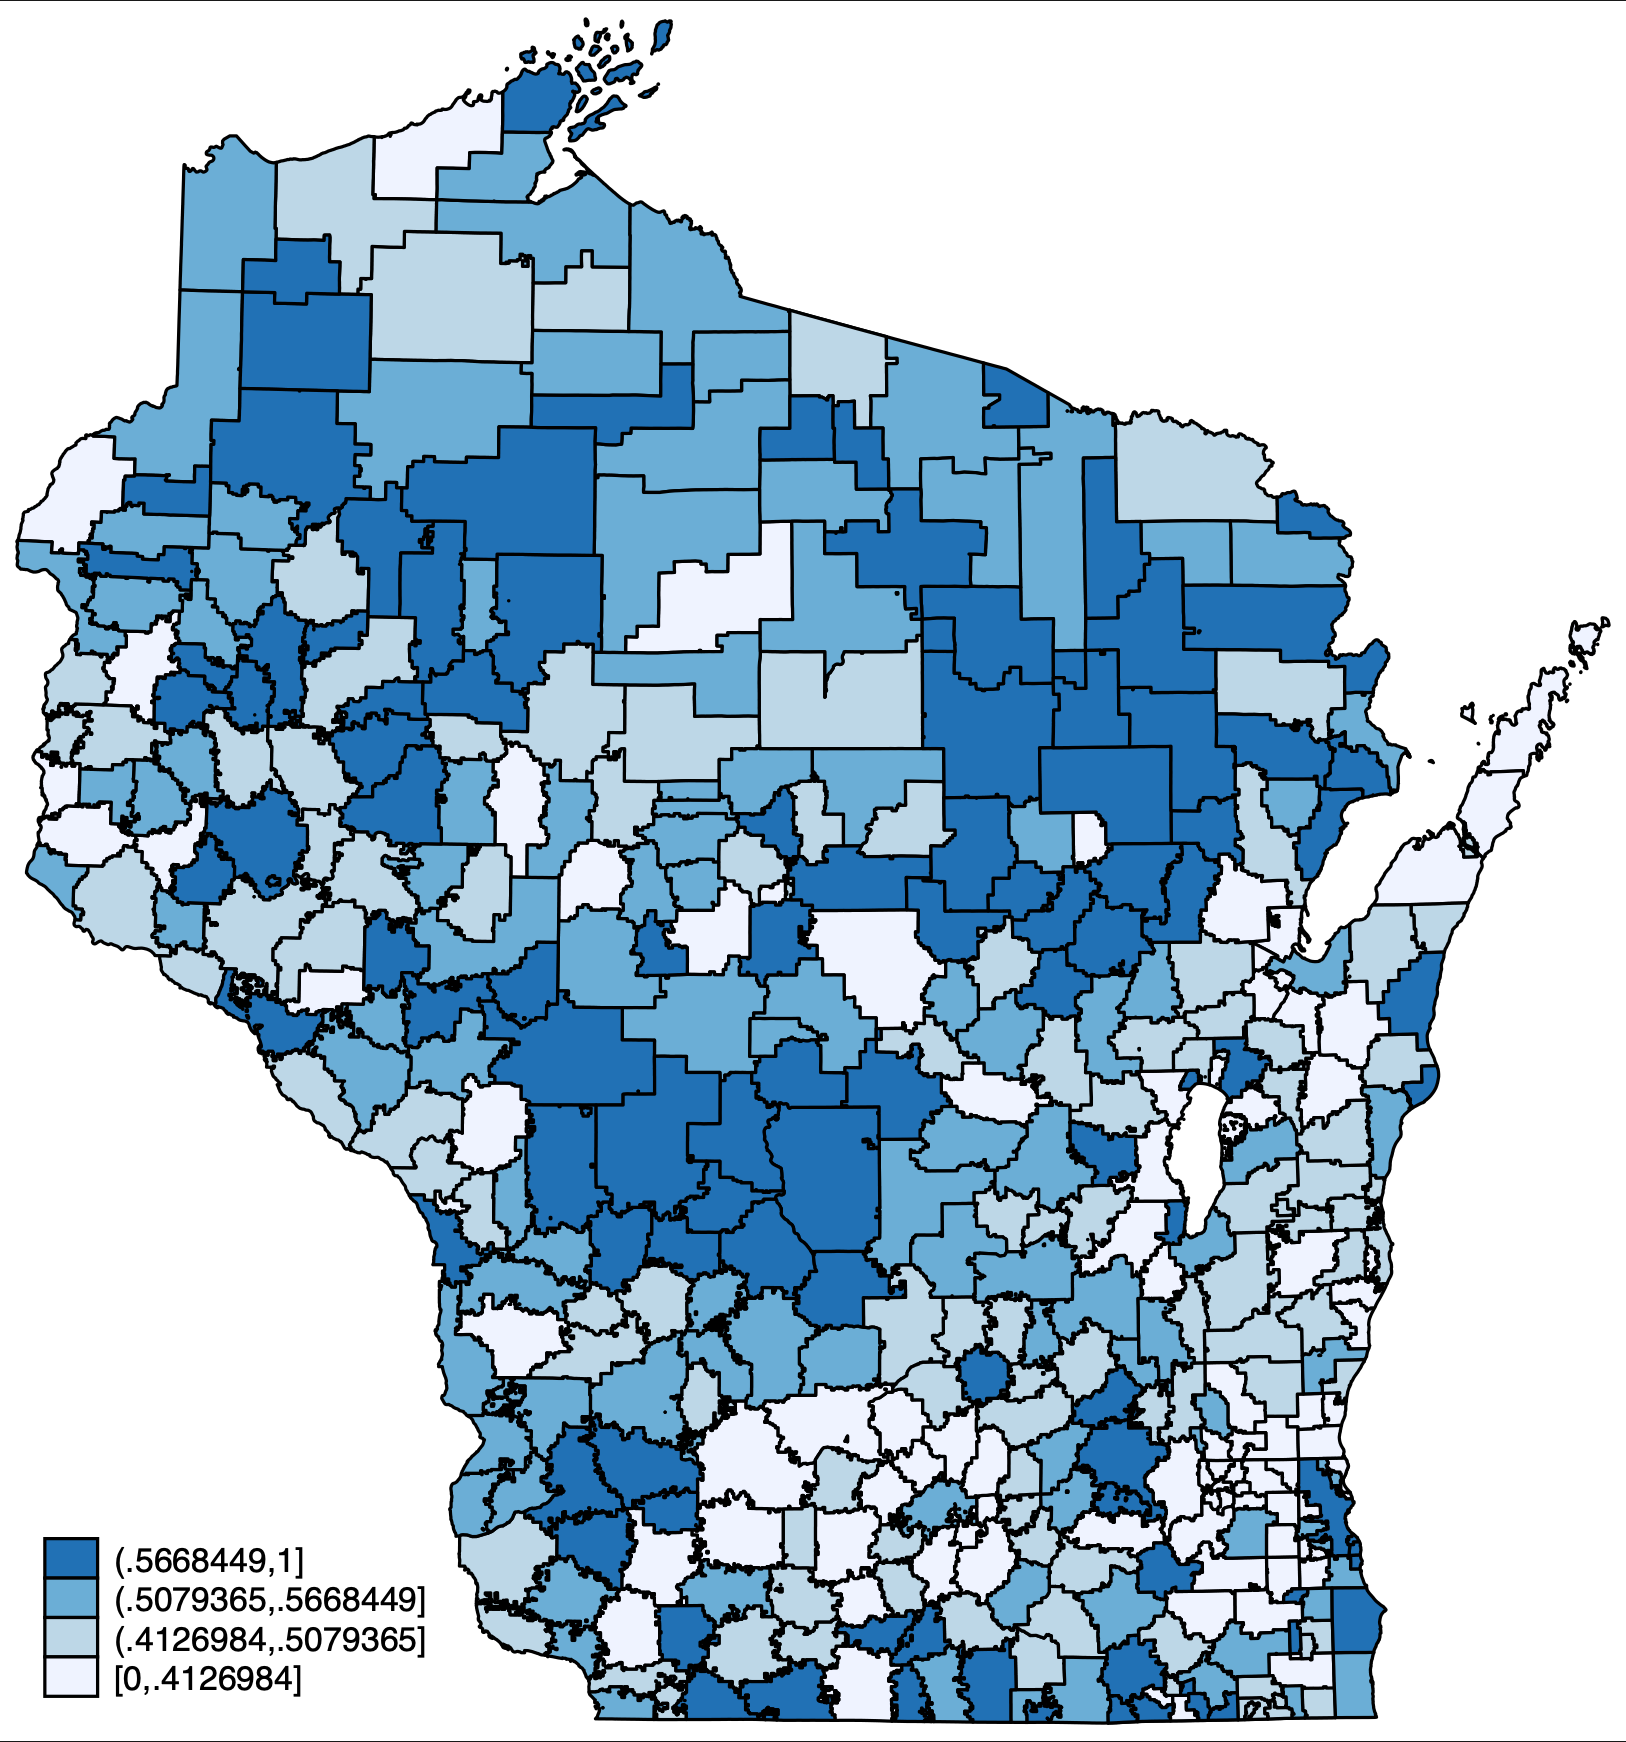
\includegraphics[width=0.7\textwidth]{figures/map.png}
\end{figure}

\nocite{wdpi_cesa}
\nocite{wdpi_school_districts_2024}
\nocite{nces_school_district_boundaries}
\nocite{bergeron_etal_2022_life_expectancy_data}
\nocite{dailykos_county_cd_overlaps_117}
\nocite{google_maps_2022}


\clearpage
\bibliographystyle{chicago}
\bibliography{biblio_wicomp}



\end{document}